%%%%%%%%%%%%%%%%%%%%%%%%%%%%%%%%%%%%%%%%%%%%%%%%%%%%%%%%%%%%%%%%
% Tipo de documento y paquetes
\documentclass[10pt]{book}
\usepackage{cdt/cdtAnalisis}
\usepackage{subfigure}
\usepackage{appendix}
\usepackage{pdfpages}
\usepackage{graphicx}
\usepackage{url}

%%%%%%%%%%%%%%%%%%%%%%%%%%%%%%%%%%%%%%%%%%%%%%%%%%%%%%%%%%%%%%%%
% Datos del proyecto
\sistema[Etapa 1]{Investigación y Desarrollo de un Modelo Ubicuo de Interoperabilidad para la Gestión de un Sistema de Información Institucional}

\documento{DA}{Documento de Análisis--Prototipo de una aplicación móvil de arquitectura offline para desastres naturales}{\DRAFT{\today}} %\RELEASE{1.0}


\fecha{\today}
\proyecto[Trabajo Terminal 2017-B017]{Trabajo Terminal 2017-B017}

\organizacion{Instituto Politécnico Nacional}

\author{Escuela Superior de Cómputo}

	\elaboro[Alumno de la ESCOM]{Eduardo Pérez Gómez}   % Responsable del contenido (IPN)
	\elaboroo[Alumno de la ESCOM]{Héctor Iván Jiménez Romero}
\superviso[Director]{M. en C. Ulises Vélez Saldaña} % Quien recibe el documento (Contraparte)
\sinI[Sinodal]{M. en C. Hermes Fransisco Montes Casiano}
\sinII[Sinodal]{M. en C. Jaime Hugo Puebla Lomas}
\sinIII[Sinodal]{M. en C. Alejandro Sigfrido Cifuentes}
\aprobo[Comité]{ } % Responsable Técnico (Contraparte)

\title{\varProyecto}
\subtitle {\varCveDocumento--\varDocumento}

%\setImgPortada{calmecacTheme/banner2}
%\setImgPleca{calmecacTheme/footer3}
%\setImgHeader{calmecacTheme/logoPar}{calmecacTheme/logoInp}
%\setImgLogo{calmecacTheme/headerInp}{calmecacTheme/headerPar}

%%%%%%%%%%%%%%%%%%%%%%%%%%%%%%%%%%%%%%%%%%%%%%%%%%%%%%%%%%%%%%%
% Elementos contenidos en el documento

%%%%%%%%%%%%%%%%%%%%%%%%%%%%%%%%%%%%%%%%%%%%%%%%%%%%%%%%%%%%%%%%
% Documentos relacionados con el documento actual

%%%%%%%%%%%%%%%%%%%%%%%%%%%%%%%%%%%%%%%%%%%%%%%%%%%%%%%%%%%%%%%%
% Inicio del Documento
\begin{document}

    %=========================================================
    % Portada
    \thispagestyle{empty}

    \maketitle
    
    %=========================================================
    % Hoja de revisión
    \makeDocInfo
    \bigskip\\
    %\makeElemRefs
    %\makeDocRefs
    \makeObservaciones[3cm]
    \vspace{2cm}
    \makeFirmas

    %=========================================================
    % Indices del documento
    \frontmatter
    \tableofcontents
    \listoffigures
    \listoftables
    \mainmatter

    %=========================================================
    % Para ocultar la información del documentador se descomenta: \hideControlVersion
    %\hideControlVersion

    %=========================================================
    % CAPÍTULOS DEL DOCUMENTO
    \chapter{Planteamiento del problema}
    \label{ch:planteamiento}
	\section{Introducción}
Cada día el uso de dispositivos móviles ha ido en aumento, y con ello el uso de aplicaciones móviles también. En 2015 hubo un aumento de 58\% en el uso de aplicaciones móviles [1], ya que actualmente los smartphones son el dispositivo favorito de 9 de cada 10 consumidores. De la misma manera en 2017 se han detectado 10 tendencias en aplicaciones móviles las cuales son: Pagos electrónicos, realidad aumentada, el aumento de Android, el uso de Bitcoins, animaciones dinámicas, internet de las cosas, aplicaciones On-Demand, inteligencia artificial, big data y aplicaciones en la nube. [2]
Así mismo mejorar los servicios que se ofrecen en el ámbito público, de modo que las tecnologías de información sirven para que la mayoría de las personas tengan acceso a este tipo de servicios y se cuente con una mejor calidad en los servicios facilitando el día a día de las personas.
En México existe una problemática y es que se encuentra dentro de una zona geográfica conocida como: Cinturón de Fuego. Esta zona hace que a lo largo del año se tenga actividad sísmica dentro del país y, aunque la mayoría de las veces estas actividades no sean alarmantes, se cuenta con un protocolo por parte de Protección Civil que debe seguirse en caso de que haya un sismo de magnitud alta. Por otro lado, México se encuentra en una zona tropical lo que provoca que en el país también lleguen huracanes y tormentas tropicales y, aunque estas sean la mayoría de las veces en zonas costeras, también debe seguirse un protocolo de Protección Civil. Sin embargo, en estos protocolos no se hace mención sobre donde pueden encontrarse refugios o albergues.
La actividad sísmica en México aumentó en cada enero de los últimos cinco años, al pasar de 490 temblores en 2014 a dos mil 575 en ese mismo tiempo de 2018, revelan datos del Servicio Sismológico Nacional (SSN).
Desafortunadamente, los desastres naturales específicamente en terremotos o sismos ya que estos siempre estarán presentes y generarán una serie de daños y consecuencias para la humanidad en el futuro. Hoy día, por ejemplo, el calentamiento global está provocando cambios climáticos y graves desastres naturales, que tienen un impacto no solo sobre la economía de las naciones y de las personas que las habitan, sino también sobre los sistemas de convivencia y de interrelación social. 
De hecho, es de esperarse que los terremotos o sismos del futuro sean de mayor magnitud e intensidad, provocando daños mayores a la economía de las naciones y de las personas, lo que hace necesario estudiar y analizar desde diferentes disciplinas estos fenómenos para mitigar sus consecuencias negativas 

Desastres Naturales 

La palabra desastre proviene del latín dis (separación) y de astro (estrella), haciendo referencia a fenómenos astrológicos anormales, que los antiguos romanos tomaban como presagio del avecinamiento de grandes males [2]. En este sentido, un desastre natural es un fenómeno anormal de la naturaleza que genera ciertos perjuicios y pérdidas para los seres humanos.
Los desastres naturales pueden clasificarse en cuatro diferentes tipos, de acuerdo con la naturaleza del desastre y la causa que los genera. Estos son los desastres hidrológicos, los meteorológicos, los geofísicos y los biológicos.
Sin embargo, en lo que se centra este trabajo terminal son en desastres geofísicos provienen de la tierra o el espacio, tales como las tormentas solares, los terremotos, las avalanchas, los derrumbes, terremotos, erupciones volcánicas y hundimientos de tierra, entre otros.

\section{Problemática}
El 80\% de las personas que habitan en la Ciudad de México desconocen los protocolos propuestos por protección civil y en muchos casos no se tiene acceso a estos ya sea por falta de tiempo o simplemente por falta de interés. Esto conlleva que a falta de esta información no sepan cómo actuar, a donde dirigirse, donde y como resguardarse cuando suceden estos tipos de desastres naturales y que es lo que se recomienda según protección civil.
\\\\Al igual desconocen información como la ubicación de los centros de recolección de víveres, refugios y albergues. Por lo tanto, la mayoría de las personas no sebe a donde dirigirse a brindar su ayuda y víveres para los afectados después de un sismo. Con esto tenemos que también no se conoce un inventario de los víveres y herramientas que se tienen en estos centros, este ha llegado a ser un problema bastante grande en los últimos sismos de magnitud grande en la Ciudad de México ya que los ciudadanos al desconocer esta información no llevan la ayuda que más se necesita e incluso no la llevan en donde realmente se necesita más.
\\\\Otro de los problemas que se presentan cuando ocurre un sismo es que no tenemos una conexión ya que se cae por completo la red por lo tanto esto provoca que cuando se quiera consultar información relacionado con desastre natural que se estuviese presentando en ese momento.
\\\\Es por eso que en este Trabajo Terminal se propone el desarrollo de un prototipo de aplicación móvil que esté basada en arquitectura offline para que pueda ser utilizada en caso de que se presente un desastre natural anteriormente mencionados y poder resolver la problemática de qué hacer cuando se presentan y a donde ir cuando se presentan.

\section{Objetivo}

\subsection{Objetivo General}
Desarrollar un sistema que proporcione a los usuarios una herramienta de alerta sísmica y de apoyo para visualizar la información de refugios, centros de recolección y albergues dados de alta en apoyo a los sismos en la Ciudad de México, mostrando una ruta a sus destinos mediante dispositivos móviles sin necesidad de una conexión a internet.

\subsection{Objetivos Específicos}
\begin{itemize}
	\item Generación de alertas sísmicas en la Ciudad de México, las cuales serán recibidas mediante frecuencias de radio.
	\item Permitir visualizar los protocolos que se deben seguir durante y después de un sismo, según protección civil.
	\item Permitir obtener la ruta hacia los refugios, centros de recolección y albergues mediante el GPS, sin necesidad de una conexión a internet.
	\item Permitir visualizar la última información de los refugios, centros de recolección y albergues tales como: ubicación, capacidad, disponibilidad de víveres y herramientas.
	\item Desarrollar un módulo de contribución a alta de refugios, centros de recolección y albergues nuevos por los usuarios, la cual deberá ser validada para su posterior publicación.
\end{itemize}


\section{Alcance}

\section{Justificación}
La necesidad que se pretende satisfacer en los usuarios de esta aplicación es la de seguridad, una definición dentro de las ciencias de la seguridad es “Ciencia interdisciplinaria que está encargada de evaluar, estudiar y gestionar los riesgos que se encuentra sometido una persona, un bien o el ambiente”. Con esto tenemos que la aplicación deberá ser capaz de alertar a los usuarios en caso de un sismo en la Ciudad de México, dejando al sistema que se encargue de informar acerca de los protocolos a seguir durante y después de un sismo, según Protección Civil. Al igual de poder brindar información de los refugios, centros de recolección y albergues, como lo es: ubicación, inventarios de víveres, inventario de herramientas, capacidad y nivel de necesidad de ayuda comunitaria, etc. Además de esto sabemos que las telecomunicaciones pueden llegar a caer durante un desastre natural como lo es un sismo, por lo que la necesidad de poder llegar a un albergue, centro de recolección o refugio es muy importante para poder salvaguardarse o brindar la ayuda a quien lo necesita, por esto es necesario tener a la mano una ruta hacia estos lugares sin la necesidad de una conexión a internet por lo que el mapeo offline será un gran punto a integrar en la aplicación. Todo esto para brindarle al usuario todas las herramientas para sobrellevar un ismo en la Ciudad de México. 

\section{Definición de términos}
	
	\chapter{Marco Teórico} 
	\label{ch:marco}
	\section{Sistemas de alarma sísmica}
Es un sistema de sensores sísmicos distribuidos en el centro y la costa oeste de México, diseñado para detectar movimientos sísmicos y emitir alertas tempranas a fin de advertir a las autoridades de protección civil y a la sociedad en general cuando ocurra un sismo que pueda afectar a ciudades vulnerables.
La alarma se activa con sismos de magnitudes cercanas a los 6 grados y se transmite en los 8 mil 200 altavoces distribuidos en las 16 delegaciones de la Ciudad de México. 
Es un sistema que genera una alerta con un tiempo de oportunidad previo al arribo de un sismo de sismos fuertes generados en las zonas sísmicas de mayor peligro para la población vulnerable, con el objetivo de contribuir a mitigar los posibles efectos. 
\begin{figure}[htbp]
	\begin{center}
		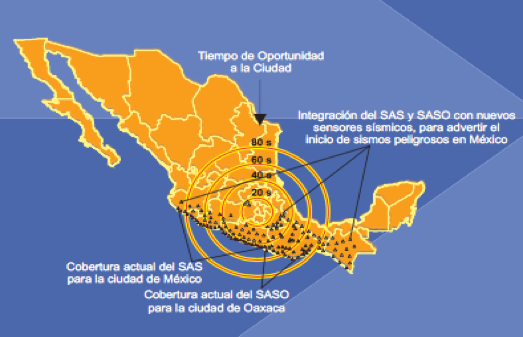
\includegraphics[width=.4\textwidth]{images/imgmarco/mapa2}
		\label{fig:mapa2}
	\end{center}
\end{figure}


\section{Transmisión de alarma sísmica}
El sistema se basa en el principio de las ondas sísmicas superficiales, las cuales son consideradas como potencialmente dañinas; éstas viajan de entre 3.5 y 4.0 kilómetros por segundo, lo que significa que tardan entre 75 y 85 segundos en viajar de Guerrero a la Ciudad de México.\\Oficialmente, la alarma se activa con sismos de magnitudes cercanas a los 6 grados y se transmite en los 8 mil 200 altavoces distribuidos en las 16 delegaciones de la Ciudad de México. \\
Para la ciudad de México es 162.450 MHz (canal 3), 162.500 MHz (canal 5) y 162.550 MHz (canal 7).
Para Acapulco y Oaxaca 162.400 MHz (canal 1).
Y Chilpancingo 162.425 MHz (canal 2).\\Los canales son para los radios de frecuencia familiar con NOAA(La Administración Nacional Oceánica y Atmosférica).
\begin{figure}[htbp]
	\begin{center}
		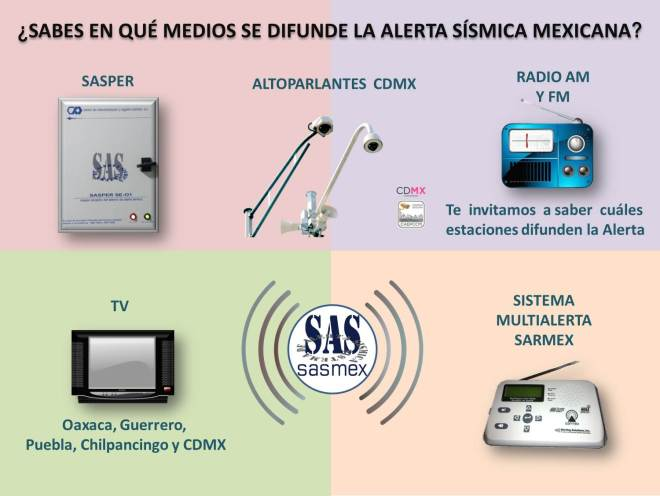
\includegraphics[width=.4\textwidth]{images/imgmarco/transmision}
		\label{fig:transmision}
	\end{center}
\end{figure}

\section{Sistema de información georeferenciado}
Un Sistema de Información Georeferenciada (GIS) es una integración organizada de hardware, software y datos geográficos diseñado para capturar, almacenar, manipular, analizar y desplegar en todas sus formas la información geográficamente referenciada con el fin de resolver problemas complejos de planificación y gestión. También puede definirse como un modelo de una parte de la realidad referido a un sistema de coordenadas terrestre y construido para satisfacer unas necesidades concretas de información.

Los SIG nos permiten hacer un análisis exhaustivo del territorio en los ámbitos más diversos. Son herramientas versátiles, con un amplio campo de aplicación en cualquier actividad que conlleve un componente espacial.
Así, la tecnología de los Sistemas de Información Geográfica puede ser utilizada para investigaciones científicas, para gestión de los recursos y activos, en arqueología, en evaluación del impacto ambiental, para la planificación urbana, en cartografía, sociología, geografía histórica, marketing o logística, por nombrar sólo algunos ámbitos de aplicación.

El SIG funciona como una base de datos con información geográfica (datos alfanuméricos) que se encuentra asociada por un identificador común a los objetos gráficos de un mapa digital. De esta forma, señalando un objeto se conocen sus atributos e, inversamente, preguntando por un registro de la base de datos se puede saber su localización en la cartografía.
La razón fundamental para utilizar un SIG es la gestión de información espacial. El sistema permite separar la información en diferentes capas temáticas y las almacena independientemente, permitiendo trabajar con ellas de manera rápida y sencilla, facilitando al profesional la posibilidad de relacionar la información existente a través de la topología de los objetos, con el fin de generar otra nueva que no podríamos obtener de otra forma.
Las principales cuestiones que puede resolver un Sistema de Información Geográfica, ordenadas de menor a mayor complejidad, son:
\begin{enumerate}
\item Localización: preguntar por las características de un lugar concreto.
\item Condición: el cumplimiento o no de unas condiciones impuestas al sistema.
\item Tendencia: comparación entre situaciones temporales o espaciales distintas de alguna característica.
\item Rutas: cálculo de rutas óptimas entre dos o más puntos.
\item Pautas: detección de pautas espaciales.
\item Modelos: generación de modelos a partir de fenómenos o actuaciones simuladas.
\end{enumerate}

\begin{figure}[htbp]
	\begin{center}
		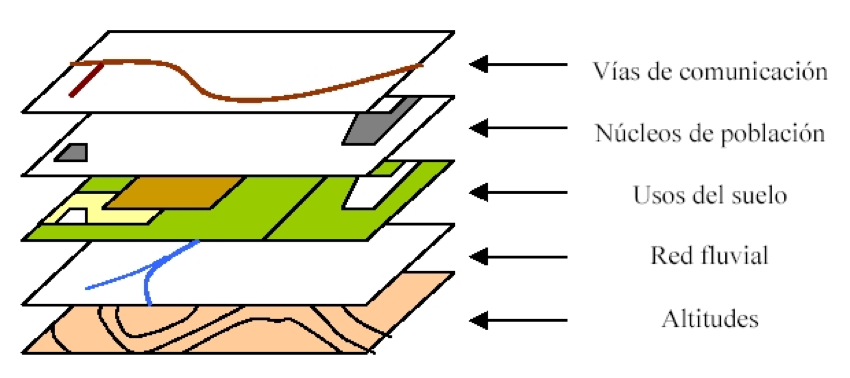
\includegraphics[width=.4\textwidth]{images/imgmarco/sistemageo}
		\label{fig:sistemageo}
	\end{center}
\end{figure}

\section{Diferencia entre Geolocalización y Georeferenciación}
Algunas de las funciones más utilizadas por los usuarios pueden ser: cómo llegar a un lugar utilizando el trayecto más corto, ubicar en el mapa nuestro próximo destino de vacaciones, o informar a algún familiar de exactamente el lugar en el que nos encontramos. A la hora de utilizar estos servicios, aparecen dos conceptos: la geolocalización y la georreferenciación.
Aunque a priori puedan parecer lo mismo, y de hecho en muchas ocasiones se utilicen indistintamente, existen varias diferencias entre los mismos, tanto en su definición como en sus aplicaciones y es importante conocerlas para poder hablar con propiedad. La georreferenciación se define como un proceso por el cual se dota de un sistema de referencia de coordenadas terreno a una imagen digital que originariamente se encuentra en coordenadas pixel.
Por su parte, la geolocalización se define como la identificación de la ubicación de un dispositivo por ejemplo un radar, dispositivo móvil o cualquier aparato tecnológico conectado a internet. Está relacionada con los sistemas de detección de posición, pero añade datos como información de la zona, calles, locales, etc.
Google posee dos plataformas muy conocidas por los usuarios: Google Earth y Google Maps, cada una asociada a uno de los términos. 
Google Earth es un sistema de georreferenciación que nos permite situar en el mapa puntos concretos de la geografía. Además, esta aplicación también nos permite obtener una vista aérea de las ubicaciones y navegar por ellas, pero son mapas creados a partir de la selección de un conjunto de datos.
La geolocalización por su parte tiene una característica muy específica: nos permite localizar un dispositivo en el mapa en tiempo real. Por ejemplo, lo que hace Google Maps es geolocalizar nuestro dispositivo, es decir, acceder a nuestra ubicación exacta y ofrecernos las diferentes funciones de la aplicación a partir de esto.
Es cierto que también tiene un sistema de georreferenciación, es decir, podemos ver planos de otros sitios distintos al que nos encontramos, pero la clave y valor añadido de la geolocalización es que a través de este sistema seremos capaces de localizar nuestro dispositivo y sobre todo de obtener información en tiempo real.

\section{GPS}
El sistema GPS (Sistema de Posicionamiento Global por sus siglas en inglés) hace posible determinar las coordenadas que permiten ubicar puntos específicos sobre la superficie de la Tierra. 
El GPS es un sistema de posicionamiento por satélites desarrollado por el Departamento de la Defensa de los E.U., diseñado para apoyar los requerimientos de navegación y posicionamiento precisos con fines militares. En la actualidad es una herramienta importante para aplicaciones de navegación, posicionamientos de puntos en tierra, mar y aire.
Hace ya varios años que los dispositivos telefónicos incorporan receptores de GPS. GPS o Sistema de Posicionamiento Global es una red compuesta por al menos 30 satélites que orbitan alrededor de la Tierra.
Al menos 4 de estos satélites estén visibles para nuestro dispositivo y cada satélite emite una señal sobre su ubicación cada cierto tiempo. Teniendo en cuenta la latitud, longitud, altura y tiempo se calcula la ubicación. Cuantos más satélites tomen parte en el proceso, más exacto será esta triangulación.
\begin{figure}[htbp]
	\begin{center}
		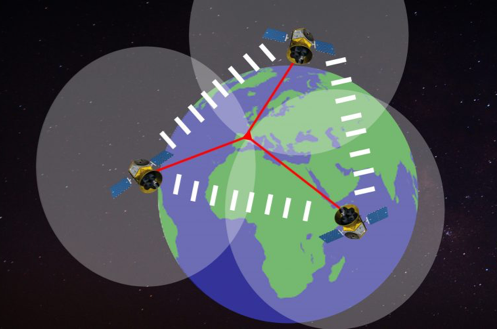
\includegraphics[width=.4\textwidth]{images/imgmarco/gps}
		\label{fig:gps}
	\end{center}
\end{figure}

\subsection{Segmento espacial}
El segmento espacial consta de una constelación de satélites que transmiten señales de radio a los usuarios.\\Los Estados Unidos mantienen la disponibilidad de no menos de 24 satélites operacionales GPS el 95% de las veces.Para garantizar este compromiso, la Fuerza Aérea ha estado volando 31 satélites GPS opercionales en los últimos años.\\
Los satélites GPS en órbita terrestreestán a una altitud media de aproximadamente 20,200 kilometros,cada satélite rodea la tierra en dos días. 
\subsubsection{2.5.1.1 Señales GPS}
Los satélites del GPS transmiten dos señales de radio de baja potencia, llamadas "L1" y "L2". Cada señal GPS contiene tres componentes de información: un código pseudoaleatorio, los datos de efemérides de satélite y datos de almanaque. El código pseudoaleatorio identifica al satélite que transmite su señal. Los datos de efemérides de satélite proporcionan información sobre la ubicación del satélite en cualquier momento. El almanaque contiene información sobre el estado del satélite y la fecha y hora actuales. Para cada satélite, el tiempo es controlado por los relojes atómicos a bordo que son cruciales para conocer su posición exacta. 


\subsubsection{2.5.1.2 Determinación de posiciones del GPS}
Aunque el GPS puede dar posiciones muy precisas, aún hay fuentes de error. Estos incluyen los errores del reloj, los retrasos atmosféricos, sin saber exactamente dónde están los satélites en sus órbitas, las señales que se refleja de los objetos en la superficie de la Tierra, e incluso la degradación intencionada de la señal del satélite. 

\subsection{Segmento de control}
Es una serie de estaciones de rastreo, distribuidas en la superficie terrestre que continuamente monitorea a cada satélite analizando las señales emitidas por estos y a su vez, actualiza los datos de los elementos y mensajes de navegación, así como las correcciones de reloj de los satélites.\\Las estaciones se ubican estratégicamente cercanas al plano ecuatorial y en todas se cuenta con receptores con relojes de muy alta precisión.
\subsection{Segmento de usuario}
Lo integran los receptores GPS que registran la señal emitida por los satélites para el cálculo de su posición tomando como base la velocidad de la luz y el tiempo de viaje de la señal, así se obtienen las pseudodistancias entre cada satélite y el receptor en un tiempo determinado, observando al menos cuatro satélites en tiempo común; el receptor calcula las coordenadas X, Y, Z y el tiempo.

\section{DGPS}
Es un sistema que proporciona a los receptores de GPS correcciones de los datos recibidos de los satélites GPS, con el fin de proporcionar una mayor precisión en la posición calculada.
El fundamento radica en el hecho de que los errores producidos por el sistema GPS afectan por igual (o de forma muy similar) a los receptores situados próximos entre sí.
\begin{figure}[htbp]
	\begin{center}
		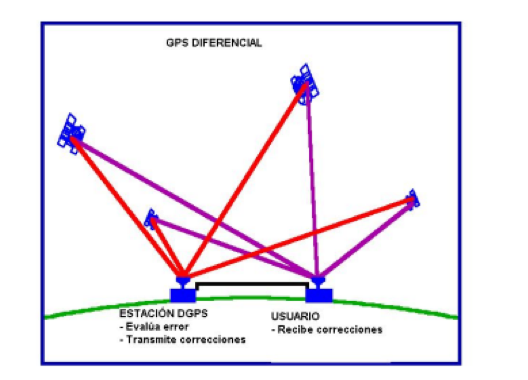
\includegraphics[width=.3\textwidth]{images/imgmarco/dgps}
		\label{fig:dgps}
	\end{center}
\end{figure}
\subsection{Estructura del DGPS}
La estructura esta de la siguiente manera:
\begin{itemize}
\item Estimación monitorizada
\item Equipo de usuario 
\item Una corrección directamente aplicada a la posición 
\item Una corrección aplicada a las pseudodistancias (Distancia media entre la antena de receptor GPS y el satélite) de cada uno de los satélites visibles.
\end{itemize}

\section{Integracion con la telefonía móvil}
Actualmente dentro del mercado de la telefonía móvil la tendencia es la de integrar, por parte de los fabricantes, la tecnología GPS dentro de sus dispositivos. El uso y masificación del GPS está particularmente extendido en los teléfonos móviles smartphone, lo que ha hecho surgir todo un ecosistema de software para este tipo de dispositivos, así como nuevos modelos de negocios que van desde el uso del terminal móvil para la navegación tradicional punto-a-punto hasta la prestación de los llamados Servicios Basados en la Localización (LBS).
Un buen ejemplo del uso del GPS en la telefonía móvil son las aplicaciones que permiten conocer la posición de amigos cercanos sobre un mapa base. Para ello basta con tener la aplicación respectiva para la plataforma deseada (Android, Bada, IOS, WP, Symbian) y permitir ser localizado por otros.

\section{Memoria Caché}
La memoria caché de un procesador, es un tipo de memoria volátil (como la memoria RAM), pero muy rápida. Su función es almacenar instrucciones y datos a los que el procesador debe acceder continuamente.\\{\bf ¿CUAL ES SU FINALIDAD?}\\Estos tipos de datos sean de acceso instantáneo para el procesador, ya que se trata de información relevante y que debe estar a la mano de manera muy fluida. Los sistemas de hardware y software llamados caché, almacenan este tipo de datos de manera duplicada y por esta razón su acceso es tan veloz.
\subsection{¿Como Funciona la memoria caché}
Cada vez que el sistema quiere acceder a un nuevo dato, éste es almacenado en la memoria caché. Entonces, cuando se necesita recurrir nuevamente al mismo dato, el sistema se dirigirá directamente al caché, haciendo así el proceso mucho más rápido. Este ciclo de almacenamiento y rescate de datos, obliga a la memoria caché a estar en continua renovación.\\Su función,es mantener de manera temporal y accesible aquellos datos que son requeridos por el sistema para realizar determinadas funciones o tareas. Así, cada vez que abras una app en tu smartphone, ésta tendrá acceso inmediato a la información que necesita para subir el nivel de eficiencia de sus funciones.
\subsection{Tipos de Memoria Caché}
Hay tres tipos de caché frecuentemente usados en computadoras personales: \\ 1.-caché de disco.\\ 2.-caché de pista.\\ 3.-caché web.\\ {\bf Caché de disco.\\}
Es una porción de memoria RAM asociada a un disco, con el fin de almacenar datos recientemente leídos y agilizar su carga en dado caso que sean solicitados otra vez. puede mejorar notablemente el rendimiento de las aplicaciones, dado que acceder a un byte de datos en RAM puede ser miles de veces más rápido que acceder a un byte del disco duro.\\
{\bf Caché de pista.\\}
Es una memoria de estado sólido tipo RAM cuyo uso de esta clase de discos generalmente se limita a las supercomputadoras por su costo tan elevado.\\
{\bf Cache web.\\}
Es la encargada de almacenar documentos web para reducir el ancho de banda consumido, la carga de los servidores y el retraso de las descargas. Existen 3 tipos de cache web: Privados que solo funcionan para un usuario, Compartidos Sirven páginas a varios usuarios y Pasarela que funcionan a cargo del propio servidor original. 
{\bf Composiciíon Interna.\\}
Los datos en la memoria caché se alojan en distintos niveles según la frecuencia de uso que tengan. La información puede transferirse entre los distintos niveles de forma inclusiva o exclusiva:\\
{\bf Caché Inclusivo.\\}
Los datos solicitados se quedan en la memoria caché de procedencia.\\
{\bf Caché Exclusivo.\\}
Los datos solicitados se eliminan de la memoria caché de procedencia una vez transferidos al nuevo nivel.\\
\subsubsection{2.8.2.1 Memoria caché nivel 1}
También llamada memoria interna, se encuentra en el núcleo del microprocesador y su capacidad es de hasta 768 kb. Es utilizada para almacenar y acceder a datos e instrucciones importantes y de uso frecuente, agilizando los procesos al ser el nivel que ofrece un tiempo de respuesta menor. Se divide en dos subniveles:\\
Nivel 1 Data Cache:\\ Se encarga de almacenar datos usados frecuentemente.\\
Nivel 1 Instruction Cache:\\ Se encarga de almacenar instrucciones usadas frecuentemente.
\subsubsection{2.8.2.2 Memoria caché nivel 2}
Se encarga de almacenar datos de uso frecuente, siendo más lenta que la caché nivel 1, pero más rápida que la memoria principal (RAM). Se encuentra en el procesador, pero no en su núcleo. Genera una copia del nivel 1.
\subsubsection{2.8.2.3 Memoria caché nivel 3}
Esta memoria genera una copia a la nivel 2. Es más rápida que la memoria principal (RAM), pero más lenta que el nivel 2. En esta memoria se agiliza el acceso a datos e instrucciones que no fueron localizadas en nivel 1 o nivel 2.\\Es generalmente de un tamaño mayor y ayuda a que el sistema guarde gran cantidad de información agilizando las tareas del procesador.\\En la actualidad esta memoria ya no es tan usada.
\section{Versiones de Android en México}
La fragmentación en Android no es un tema nuevo, aquí hemos expresado nuestra opinión más de una vez, y a pesar de que es el sistema operativo que más me gusta, cada mes queda muy claro que a Google le urge encontrar una solución para obligar o ayudar a los fabricantes a actualizar sus dispositivos.\\En el reporte de diciembre del 2017  vemos como {\bf Android Oreo} apenas está en el 0.5 porciento de todos los dispositivos del mercado, mientras que {\bf Android Nougat} que ya lleva poco más de un año alcanza ya el 23.3 porciento de cuota, sin embargo, {\bf Android 6.0 Marshmallow} tiene el 29.7 porciento y {\bf Android 5.0 Lollipop} que ya tiene más de tres años disponible está presente en el 26.3 porcirnto de smartphones con Android.
\begin{figure}[htbp]
	\begin{center}
		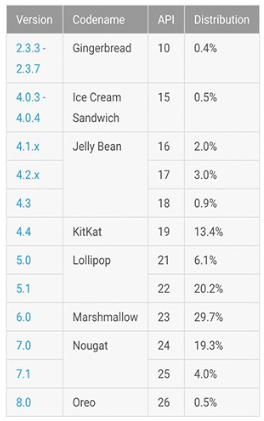
\includegraphics[width=.3\textwidth]{images/imgmarco/versiones}
		\label{fig:versiones}
	\end{center}
\end{figure}


\section{Diferencia entre GDP y DGPS}
El Sistema de Posicionamiento Global Diferencial (DGPS) es una mejora para el GPS (Sistema de Posición Global). El sistema GPS basado en la tecnología satelital puede tener una precisión nominal de 15 metros, mientras que DGPS puede alcanzar una precisión de alrededor de 10 cm. [16] DGPS usa las estaciones de referencia fijas basadas en tierra para transmitir la diferencia entre las coordenadas del GPS y la posición fija desde la estación base. La señal de corrección digital se transmite a todos los transmisores basados en tierra llamados rovers. El DGPS se basa en dos estaciones, una es la estación base y la siguiente es el usuario. 

\section{Mapas interactivos}
Los mapas interactivos que se encuentran disponibles en Internet incluyen: los geográficos, desarrollados por Google y Microsoft, los cuales proveen la funcionalidad de definir puntos de localización de puntos de interés. Sin embargo, estos mapas, en su versión satelital, tienen la limitante de que las imágenes no son actualizadas con regularidad. Por otro lado, plataformas como MapBox permite la creación de mapas interactivos. Mapbox es una plataforma que permite el desarrollo de aplicaciones móviles y aplicaciones web para la creación de mapas que permitan la localización de datos, incluyendo, además de los diseños de mapas satelitales y de calles, diseños de mapas de terrenos y tráfico [MapBox, s.f.]. MapBox ofrece un plan de costos que varía de acuerdo al número de vistas y solicitudes de información. 
En MapBox todo es 100% personalizable. Desde cualquier color hasta mostrar/ocultar capas en el mapa. Hay una serie de estilos disponibles por defecto (Dark, Light, etc.) pero también tienes la posibilidad de diseñar/crear tus propios estilos por completo a través de la herramienta Mapbox Studio. 
Todo el código está abierto y basado en estándares abiertos. Mapbox dispone de más de 500 repositorios en Github. 
No importa para qué plataforma desarrolles porque hay SDKsdisponibles para prácticamente todas. Entre las cuales están Android, iOS, Web, Qt, Unity y MacOS. Además, todas las funcionalidades están accesibles desde cada uno de ellos, ya que comparten una misma base.
Todo ocurre en tu app. No hay necesidad de tener que saltar a otra aplicación para nada (Mapbox no tiene apps para usuarios así que no tiene interés en competir con sus desarrolladores). Esto es especialmente útil si estás desarrollando una app de navegación, ya que, a diferencia de otros SDKs, puedes proveer una experiencia de navegación completa, sin perder a tus usuarios en ningún momento. Otro ejemplo es la posibilidad de guardar mapas offline sin salir de tu app.
El core está basado en mapas vectoriales implementados en C++, de forma que únicamente se mandan los datos necesarios al dispositivo y se interpretan en tiempo real, lo que se traduce en mapas muy rápidos y en visualizaciones mucho más ligeras.
Tanto el SDK de Android como el de iOS tienen una API similar a la de Google Maps y MapKit respectivamente.

\subsection{Mapas offline}
El uso de aplicaciones que puedan seguir funcionando sin conexión a internet es una característica muy importante a la hora de hablar de aplicaciones de mapeo. El poder acceder a una lista de mapas almacenados en nuestro dispositivo y eliminar los que ya no necesitemos es una opción muy atractiva para no gastar los datos de nuestro servicio de internet o en el peor caso que no tengamos red debido a que nos encontremos en un lugar sin cobertura de señal o que debido a un suceso independiente de nosotros y de nuestra compañía de servicio de internet las telecomunicaciones fallen y podamos hacer uso de esta funcionalidad sin ningún problema. 
Al poder tener esta opción de guardar regiones del mapa en nuestro dispositivo tenemos que considerar algunas cosas como que una región fuera de línea no se puede modificar después de la creación, pero es posible crear una nueva región con una definición modificada y eliminar la ya existente. Al igual una región abarca cierta dimensión, y que una vez guardada no se puede modificar, por lo que tenemos que tener en cuenta que las ubicaciones que busquemos fuera de este rango será imposible encontrarlas. Y que se tiene que considerar poder guardar en nuestro dispositivo cierta cantidad de regiones para no saturar el espacio de almacenamiento del mismo.

\section{Estado del arte}
SKY ALERT:\\CARACTERÍSTICAS\\1.-Tiene sus propios sensores de alertas sismicas.\\2.-Alerta de tormentas,Contingencias,Tsunamis y Alertas volcanicas.\\3.-Cuenta con programa de simulacro.\\4.-Cuenta con publicaciones en las redes sociales.\\5.-Requiere de una conexión a Internet.\\6.-No cuenta con repetidora de señal por estacion de radio(NOAA).\\7.-Alerta Sísmicas.\\8.- No cuenta con notificaciones push para alertas sísmicas.\\9.-No cuenta con mapeo de ruta hasta un lugar seguro.\\10.-No proporciona información de albergues.\\11.-No te deja ver mapas de albergues,refugios,centros de acopio.\\ 
\\

911 CDMX:\\CARACTERÍSTICAS\\1.-No tiene sus propios sensores de alertas sismicas.\\2.-No Alerta de tormentas,Contingencias,Tsunamis y ni de Alertas volcanicas.\\3.-No cuenta con programa de simulacro.\\4.-Cuenta con publicaciones en las redes sociales.\\5.-Requiere de una conexión a Internet.\\6.-Si cuenta con repetidora de señal por estacion de radio(NOAA).\\7.-Alerta Sísmicas.\\8.-No cuenta con notificaciones push para alertas sísmicas.\\9.-No cuenta con mapeo de ruta hasta un lugar seguro.\\10.-No proporciona información de albergues.\\11.-No te deja ver mapas de albergues,refugios,centros de acopio.\\
\\

ALERTA SÍSMICA DF:\\CARACTERÍSTICAS\\1.-No tiene sus propios sensores de alertas sismicas.\\2.-No Alerta de tormentas,Contingencias,Tsunamis y ni de Alertas volcanicas.\\3.-Cuenta con programa de simulacro.\\4.-No cuenta con publicaciones en las redes sociales.\\5.-Requiere de una conexión a Internet.\\6.-Si cuenta con repetidora de señal por estacion de radio(NOAA).\\7.-No proporciona una alerta Sísmicas.\\8.-Cuenta con notificaciones push para alertas sísmicas.\\9.-No cuenta con mapeo de ruta hasta un lugar seguro.\\10.-No proporciona información de albergues.\\11.-No te deja ver mapas de albergues,refugios,centros de acopio.\\
\\


SOLUCIÓN PROPUESTA:\\CARACTERÍSTICAS\\1.-No tiene sus propios sensores de alertas sismicas.\\2.-No Alerta de tormentas,Contingencias,Tsunamis y ni de Alertas volcanicas.\\3.-Cuenta con programa de simulacro.\\4.-No cuenta con publicaciones en las redes sociales.\\5.-No requiere de una conexión a Internet.\\6.-No cuenta con repetidora de señal por estacion de radio(NOAA).\\7.-Cuenta con Alerta Sísmicas.\\8.-Cuenta con notificaciones push para alertas sísmicas.\\9.-Cuenta con mapeo de ruta hasta un lugar seguro.\\10.-Proporciona información de albergues.\\11.-Te deja ver mapas de albergues,refugios,centros de acopio.\\
\\
DEFINICIONES:\\ \\
SKY ALERT: Es una de las herramientas con lo cual se podrá atento a cualquier movimiento telúrico y otros fenomenos naturales.\\ La plataforma tiene cobertura en la Ciudad de México, Estado de México,Puebla,Morelos,Michoacan,Guerrero,Tlaxcala,Jalisco,Colima Oaxaca  y Chiapas.\\
\\
911 CDMX: Es una aplicación para teléfonos inteligentes con sistema operativo iOS o Android, que conecta a las y los usuarios directamente al 9-1-1 de la Ciudad de México, puede ser por llamada telefónica y por chat. Además cuenta con la Alerta Sísmica, la cual se activará cuando se detecte algún sismo que por su magnitud ponga en riesgo a la CDMX.\\
\\
ALERTA SÍSMICA DF: Es una aplicación de alerta temprana que recibe notificaciones push con avisos de actividad sísmica y recibe noticias relevantes relacionadas con protección civil.\\
\\
SOLUCIÓN DE PROPUESTA: Es una aplicacion de alerta sísmica con lo cual te alertará de cualquier movimiento sísmico a tráves de notificaciones push, la aplicación tambien proporciona información de refugios ,albergues y centros de acopio ubicados en la CDMX.\\La aplicación brinda la oprtunidad de que realices tu propio registro de refugio, albergue y centro de acopio y cuenta con mapeo de ruta hasta un albergue o refugio.
	
	
	
	%========Modelo del Alcance ===== %
	%Se comenta para el reporte tecnico	
	%\part{Modelo del Alcance}
	
	% Requerimientos funcionales y no funcionales
	%\section{Requerimientos Funcionales}
	%\label{chapter:UC}	
	%%\cdtInstrucciones{
	%Identifique y describa los requerimientos funcionales del sistema señalando: id, nombre, descripción y prioridad.
%}
\begin{requerimientos}[color]
		\RFitem{RF01}{Registrar Usuario}{El Ciudadano necesita un medio por el cual pueda llevar a cabo su registro dentro del sistema SIEMS.}
		\RFitem{RF02}{Inicio De Sesión}{El Ciudadano necesita un medio por el cual pueda ingresar al sistema.}
		\RFitem{RF03}{Recuperar Contraseña}{El ciudadano requiere de un medio por el cual tenga la opcion de recuprerar su contraseña ya sea por olvido.}
		\RFitem{RF04}{Cerrar Sesión}{El Ciudadano requiere de un medio por el cual tenga la opción de cerrar la sesión en el sistema.}
		\RFitem{RF05}{Gestionar Propuestas}{El El Subsecretario de Educación Pública (administrador) necesita un medio para administrar las propuestas del ciudadano.}
		\RFitem{RF06}{Gerstionar propuesta de albergue }{El Subsecretario de Educación Pública (administrador) requiere de un medio para autorizar un albergue que propuso el ciudadano.}
		\RFitem{RF07}{Gestionar Propuesta de Refugio}{El Subsecretario de Educación Pública (administrador) requiere un medio por el cual pueda agregar un Refugio.}
		\RFitem{RF08}{Gestionar Mapas Offline}{El Cudadano requiere un medio por el cual pueda descargar y ver los mapas de modo offline.}
		\RFitem{RF09}{Gestionar Alarmas Sísmicas}{El ciudadano requiere de un medio por el cual pueda configurar las alarmas sísmicas de acuerdo a su preferencia.}
		\RFitem{RF10}{Agrega Albergue}{El Subsecretario de Educación Pública (administrador) requiere de un medio por el cual pueda agregar un albergue de tal modo ya este autorizado.}
		\RFitem{RF11}{Agrega Refugio}{El Subsecretario de Educación Pública (Administrador) requiere de un medio por el cual pueda agregar un refugio que l mismo registre o que ya este propuesto por el ciudadano .}
		\RFitem{RF12}{Mostrar Refugios,Albergues y centros de acopio}{El Ciudadano requiere de un medio para poder visualizar los refugios,albergues y centros de acopio.}
		\RFitem{RF13}{Configuración de cuenta}{El cuidadano requiere un medio por el cual el pueda configurar su cuenta en el sistema.}
		\caption{Requerimientos funcionales del sistema.}
    
    {\footnotesize\em Para leer correctamente esta tabla vea la leyenda en la Tabla~\ref{tbl:leyendaRF} en la página~\pageref{tbl:leyendaRF}.}
    \label{tbl:reqFunc}
\end{requerimientos}

\begin{requerimientos}[color]
		\RFitem{RNF01}{Compatibilidad en Androdi}{La aplicación para que funciones correctamente en los dispositivos con sistema operativo android con la versión de 5.0 llamada Lallipop y sus posteriores versiones ya que apartir de esa versión soporta la bibliotecas recientes de MapBox.}
		\RFitem{RNF02}{IDE de Desarrollo}{Para la implementación de la aplicación movil se va a utilizar un IDE gratuito en Android Studio y el Framework Laravel de php para la implementación de la página web.}
		\RFitem{RNF03}{Gestor de Base de Datos}{El gestor de base de datos utilizado sera Firebase ya que proporciona datos en tiempo real y utiliza REST API el cual es una API que para crear conexiones de HTTP para recibir notificaciones push de un servisor.}
		\RFitem{RNF04}{Compatibilidad de Navegadores}{La Aplicación web va a funcionar con navegadores que soporten mapas de la API MapBox.}
		\caption{Requerimientos no funcionales del sistema.}            {\footnotesize\em Para leer correctamente esta tabla vea la leyenda en la Tabla~\ref{tbl:leyendaRF} en la página~\pageref{tbl:leyendaRF}.}
    \label{tbl:reqNoFunc}
\end{requerimientos}
	
	%\section{Requerimientos No Funcionales}
	%\label{chapter:UC}	
	%%\cdtInstrucciones{
	%Identifique y describa los requerimientos funcionales del sistema señalando: id, nombre, descripción y prioridad.
%}
\begin{requerimientos}[color]
		\RFitem{RF01}{Registrar Usuario}{El Ciudadano necesita un medio por el cual pueda llevar a cabo su registro dentro del sistema SIEMS.}
		\RFitem{RF02}{Inicio De Sesión}{El Ciudadano necesita un medio por el cual pueda ingresar al sistema.}
		\RFitem{RF03}{Recuperar Contraseña}{El ciudadano requiere de un medio por el cual tenga la opcion de recuprerar su contraseña ya sea por olvido.}
		\RFitem{RF04}{Cerrar Sesión}{El Ciudadano requiere de un medio por el cual tenga la opción de cerrar la sesión en el sistema.}
		\RFitem{RF05}{Gestionar Propuestas}{El El Subsecretario de Educación Pública (administrador) necesita un medio para administrar las propuestas del ciudadano.}
		\RFitem{RF06}{Gerstionar propuesta de albergue }{El Subsecretario de Educación Pública (administrador) requiere de un medio para autorizar un albergue que propuso el ciudadano.}
		\RFitem{RF07}{Gestionar Propuesta de Refugio}{El Subsecretario de Educación Pública (administrador) requiere un medio por el cual pueda agregar un Refugio.}
		\RFitem{RF08}{Gestionar Mapas Offline}{El Cudadano requiere un medio por el cual pueda descargar y ver los mapas de modo offline.}
		\RFitem{RF09}{Gestionar Alarmas Sísmicas}{El ciudadano requiere de un medio por el cual pueda configurar las alarmas sísmicas de acuerdo a su preferencia.}
		\RFitem{RF10}{Agrega Albergue}{El Subsecretario de Educación Pública (administrador) requiere de un medio por el cual pueda agregar un albergue de tal modo ya este autorizado.}
		\RFitem{RF11}{Agrega Refugio}{El Subsecretario de Educación Pública (Administrador) requiere de un medio por el cual pueda agregar un refugio que l mismo registre o que ya este propuesto por el ciudadano .}
		\RFitem{RF12}{Mostrar Refugios,Albergues y centros de acopio}{El Ciudadano requiere de un medio para poder visualizar los refugios,albergues y centros de acopio.}
		\RFitem{RF13}{Configuración de cuenta}{El cuidadano requiere un medio por el cual el pueda configurar su cuenta en el sistema.}
		\caption{Requerimientos funcionales del sistema.}
    
    {\footnotesize\em Para leer correctamente esta tabla vea la leyenda en la Tabla~\ref{tbl:leyendaRF} en la página~\pageref{tbl:leyendaRF}.}
    \label{tbl:reqFunc}
\end{requerimientos}

\begin{requerimientos}[color]
		\RFitem{RNF01}{Compatibilidad en Androdi}{La aplicación para que funciones correctamente en los dispositivos con sistema operativo android con la versión de 5.0 llamada Lallipop y sus posteriores versiones ya que apartir de esa versión soporta la bibliotecas recientes de MapBox.}
		\RFitem{RNF02}{IDE de Desarrollo}{Para la implementación de la aplicación movil se va a utilizar un IDE gratuito en Android Studio y el Framework Laravel de php para la implementación de la página web.}
		\RFitem{RNF03}{Gestor de Base de Datos}{El gestor de base de datos utilizado sera Firebase ya que proporciona datos en tiempo real y utiliza REST API el cual es una API que para crear conexiones de HTTP para recibir notificaciones push de un servisor.}
		\RFitem{RNF04}{Compatibilidad de Navegadores}{La Aplicación web va a funcionar con navegadores que soporten mapas de la API MapBox.}
		\caption{Requerimientos no funcionales del sistema.}            {\footnotesize\em Para leer correctamente esta tabla vea la leyenda en la Tabla~\ref{tbl:leyendaRF} en la página~\pageref{tbl:leyendaRF}.}
    \label{tbl:reqNoFunc}
\end{requerimientos}
	
	
	
	%========Modelo del Negocio ===== %
     %Se comenta para el reporte tecnico	
	%\part{Modelo del Negocio}
	% Glosario
	%\chapter{Glosario}
	%\label{chapter:glosario}
	%\section{Glosario de términos}

	Esta sección describe de forma breve y sencilla los términos que son usados a lo largo del documento y que se consideran necesario para ayudar a comprender la jerga utilizada.


	
\begin{bGlosario}
	
	%\bTerm{Alta}{Alta} Documento que acredita y reconoce la inscripción. %MP DAE
	
	\bTerm{AlbergueRegistradoEnSEIMS}{Albergue Registrado en SEIMS} Albergue reconocido por el Sistema Nacional de Protección Civil, para su gestion y control vía internet.\\%SNPC
	
	\bTerm{RefugioRegistradoEnSEIMS}{Refugio Registrado en SEIMS:} Refugio reconocido por el Sistema Nacional de Protección Civil, para su gestion y control vía internet.\\
	\bTerm{CentroAcopioRegistradoEnSEIMS}{Centro de acopio Registrado en SEIMS:} Albergue reconocido por el Sistema Nacional de Protección Civil, para su gestion y control vía internet.\\
	\bTerm{MapaRegistradoEnSEIMS}{Mapa Registrado en SEIMS:} Mapa reconocido por el Sistema Nacional de Protección Civil, para su gestion y control vía internet.\\
	\bTerm{MapaDescargadoDeSEIMS}{Mapa Descargado De SEIMS} Mapa Descargado de SEIMS reconocido por el Sistema Nacional de Protección Civil, para su gestion y control via offline.

	

	
	% TODO:Agregar fuente
	
 
\end{bGlosario}



				%Glosario de términos técnicos y del negocio
	
	%\chapter{Notación, símbolos y convenciones utilizadas}
	%\label{chapter:notacion}
	%{\bf Los requerimientos funcionales utilizan una clave RFX}, donde:
	
\begin{description}
	\item[X] Es un número consecutivo: 1, 2, 3, ...
	\item[RF] Es la clave para todos los {\bf R}equerimientos {\bf F}uncionales.\\
\end{description}



	{\bf Los requerimientos del usuario utilizan una clave RUX}, donde:
	
\begin{description}
	\item[X] Es un número consecutivo: 1, 2, 3, ...
	\item[RU] Es la clave para todos los {\bf R}equerimientos del {\bf U}suario.\\
\end{description}



{\bf Los Requerimientos No Funcionales utilizan una clave RNFX},donde:
\begin{description}
	\item[X] Es un número consecutivo: 1, 2, 3, ...
	\item[RNF] Es la clave para todos los {\bf R}equerimientos {\bf N}o {\bf F}uncionales.\\
\end{description}



{\bf Las Reglas de Negocio utilizan una clave RPCX}, donde:
\begin{description}
\item[X] Es un número consecutivo:1,2,3,....
\item[RPC] Es la clave para todos los {\bf R}eglas {\bf P}rotección {\bf C}ivil.\\
\end{description}



{\bf Los Casos de Uso  utilizan una clave CUX},donde:

\begin{description}
	\item[X] Es un número consecutivo: 1, 2, 3, ...
	\item[CU] Es la clave para todos los {\bf C}asos de {\bf U}so.\\
\end{description}


DISEÑO DE INTERFACES:\\
{\bf Las Interfaces de Usuario utilizan una clave IUX},donde:

\begin{description}
	\item[X] Es un número consecutivo: 1, 2, 3, ...
	\item[IU] Es la clave para todas las {\bf I}nterfaces  de {\bf U}suario.\\
\end{description}

{\bf Los Mensages  utilizan una clave MSGX},donde:

\begin{description}
	\item[X] Es un número consecutivo: 1, 2, 3, ...
	\item[MSG] Es la clave para todos los {\bf M}ensages.\\
\end{description}

	Además, para los requerimeitnos funcionales se usan las abreviaciones que se muestran en la tabla~\ref{tbl:leyendaRF}.
\begin{table}[hbtp!]
	\begin{center}
    \begin{tabular}{|r l|}
	    \hline
    	{\footnotesize Id} & {\footnotesize\em Identificador del requerimiento.}\\
    	{\footnotesize Pri.} & {\footnotesize\em Prioridad}\\
    	{\footnotesize Ref.} & {\footnotesize\em Referencia a los Requerimientos de usuario.}\\
    	{\footnotesize MA} & {\footnotesize\em Prioridad Muy Alta.}\\
    	{\footnotesize A} & {\footnotesize\em Prioridad Alta.}\\
    	{\footnotesize M} & {\footnotesize\em Prioridad Media.}\\
    	{\footnotesize B} & {\footnotesize\em Prioridad Baja.}\\
    	{\footnotesize MB} & {\footnotesize\em Prioridad Muy Baja.}\\
		\hline
    \end{tabular} 
    \caption{Leyenda para los requerimientos funcionales.}
    \label{tbl:leyendaRF}
	\end{center}
\end{table}

	
	% Modelo de Información
	
	%\chapter{Modelo de Información} %Diagrama de Clases
	%\label{chapter:modeloInformacion}
	%% Modelo Estructural
	
	
	%Reglas de Negocio
	\chapter{Reglas de Negocio} % Reglas de Negocio
	\label{chapter:rn}
	% No comentar las reglas cuyo estatus es APROBADO.
%Ejemplo de regla de negocio
%Este documento llamará a las reglas
\section{Introducción al Capítulo}

\section{Reglas de Protección Civil}
%\begin{BusinessRule}{BR100}{Recibo del Estudiante por inscripción a Seminario.}{
		Regla de operación, (calcular o determinar un valor.).
		% Otras opciones para tipo: 
		% - Regla de integridad referencial o estructural. 
		% - Regla de operación, (calcular o determinar un valor.).
		% - Regla de inferencia de un hecho.
	}{
		Habilitadora. 
		% Otras opciones para clase: Habilitadora, Cronometrada, Ejecutive.
	}{
		Controla la operación. % Otras opciones para nivel: Controla la operación, Influencia (dirige) la operación.
	}
	\BRItem[Descripción:] El  Recibo del Estudiante debe mostrar el total del costo con el siguiente desglose:
	\begin{displaymath}\begin{array}{lr}
	Costo: & \$ XXX.XX\\
	Descuento~aplicado~(YY\%): & \$ XXX.XX\\
	Subtotal: & \$ XXX.XX\\
	IVA~(16\%): & \$ XXX.XX\\\hline
	Total: & \$ XXX.XX
	\end{array}\end{displaymath}
	\BRItem[Sentencia:] $CostoTotal = Costo(e, s) + Impuesto(e, s)$.
	\BRItem[Ejemplo positivo:] 
	
	\BRItem[Ejemplo negativo:] 
	
	\BRItem[Referenciado por:] 
\end{BusinessRule}
%\input{negocio/Reglas/BR101}
\begin{BusinessRule}{RPC101}{CONDICIONES DE UN REFUGIO.}{
		Regla de inferencia de un hecho.
		% Otras opciones para tipo: 
		% - Regla de integridad referencial o estructural. 
		% - Regla de operación, (calcular o determinar un valor.).
		% - Regla de inferencia de un hecho.
	}{
		Habilitadora. 
		% Otras opciones para clase: Habilitadora, Cronometrada, Ejecutive.
	}{
		Controla la operación. % Otras opciones para nivel: Controla la operación, Influencia (dirige) la operación.
	}
	\BRItem[Descripción:] Indentificar una instalacion como albergue temporal depende de algunos factores elementales, lo cual le permitirá garantizar una oportuna y eficaz protección a la ciudadania ante la inminecia de un peligro .Como las Siguientes\\1.-LAS CONDICIONES DE LA INSTALACIÓN: \\1.1.-influye en el tipo de construcción y estado de mantenimiento constructivo de la instalación.\\1.2.-Disponibilidad y condiciones de los servicios sanitarios y para lavado de ropa elemental necesidad, fundamentalmente de niños.\\1.3.-Numero de personas que puede refugiar partiendo de las normas que se establecen en estos lineamientos. \\2.-DISPONIBILIDAD DE SERVICIOS:\\2.1.-En la disponibilidad de lso servicios juega un ppel muy importante el volumen de agua para el consumo humano, laproporción adecuada de las instalaciones sanitarias y su estado, así como la distribución final de residuales líquidos y el tratamiento a los desechos sólidos. \\3.-CAPACIDAD DE REFUGIO.\\3.1.-La Organización Mundial de la Salud (OMS) recomienda que para alojamiento de emergencia se de debe garantizar como norma 3.5 metros cuadrados por persona , no incluyendo en ello areas recreatvas , cocinas , baños , comedor y alamacenes.
	%\BRItem[Ejemplo positivo:] 
	
	%\BRItem[Ejemplo negativo:] 
	
	\BRItem[Referenciado por:] LA GACETA OFICIAL DE LA CIUDAD DE MÉXICO , SECRETARIA DE PROTECCION CIVIL"NORMA TÉCNICA COMPLEMENTARIA NTCPC-007-ALERTAMIENTO SÍSMICO-2017"
\end{BusinessRule}
\begin{BusinessRule}{RPC102}{CONDICIONES DE UN ALBERGUE.}{
		Regla de inferencia de un hecho.
		% Otras opciones para tipo: 
		% - Regla de integridad referencial o estructural. 
		% - Regla de operación, (calcular o determinar un valor.).
		% - Regla de inferencia de un hecho.
	}{
		Habilitadora. 
		% Otras opciones para clase: Habilitadora, Cronometrada, Ejecutive.
	}{
		Controla la operación. % Otras opciones para nivel: Controla la operación, Influencia (dirige) la operación.
	}
	\BRItem[Descripción:] Para la evalucón de los albergues existe un grupo llamado "COMISIÓN DE ALBERGUE" nombrado por el director del organismo a la cual pertenece, son quienes revisan periodicamente y durante la fase informativa las condicones generales y recursos.\\De acuerdo a la COMISIÓN DE ALBERGES.\\1.-Debe contar con alojamiento y protección.\\2.-Alimentación.\\3.-Vesturio.\\4.-Recreación y esparcimiento.\\5.- Atención medica.\\6.- Seguridad.\\7.-Higiene y Saneamiento.\\8.-La Organización Mundial de la Salud (OMS) recomienda que para alojamiento de emergencia se de debe garantizar como norma 3.5 metros cuadrados por persona , no incluyendo en ello areas recreatvas , cocinas , baños , comedor y alamacenes.\\EXISTEN TRES TIPOS DE ALBERGUE:\\1.- Albergue familiar.\\2.-Albergue comunitario en instalación cerrada.\\3.-Albergue tipo cabaña. 
	%\BRItem[Ejemplo positivo:] 
	
	%\BRItem[Ejemplo negativo:] 
	
	\BRItem[Referenciado por:] LA GACETA OFICIAL DE LA CIUDAD DE MÉXICO , SECRETARIA DE PROTECCION CIVIL"NORMA TÉCNICA COMPLEMENTARIA NTCPC-007-ALERTAMIENTO SÍSMICO-2017"
\end{BusinessRule}
\begin{BusinessRule}{RPC103}{CONDICIONES DE UN CENTRO DE ACOPIO.}{
		Regla de inferencia de un hecho.
		% Otras opciones para tipo: 
		% - Regla de integridad referencial o estructural. 
		% - Regla de operación, (calcular o determinar un valor.).
		% - Regla de inferencia de un hecho.
	}{
		Habilitadora. 
		% Otras opciones para clase: Habilitadora, Cronometrada, Ejecutive.
	}{
		Controla la operación. % Otras opciones para nivel: Controla la operación, Influencia (dirige) la operación.
	}
	\BRItem[Descripción:] Es un espacio físico, instalados por las organizaciones e instancias públicas, privadas y sociales para recibir la ayuda humanitaria, cuando ésta es requerida oficialmente.\\La apertura de un centro de acopio se efectúa cuando la autoridad administradora de una emergencia lo determina, previa evaluación de los daños y recursos existentes para la atención de la población afectada o damnificada por una emergencia. \\Los centros de acopio deberán recibir insumos de acuerdo con lo señalado en las sugerencias para los donantes. Estableciendo parámetros como, tipo de producto, peso, volumen y dimensionar las necesidades y tipo de transporte requerido para su traslado.\\A continuación se dan algunas consideraciones que deberán reunir los artículos:\\1.-Ropa , zapatos y vestimenta.\\2.-Medicamentos.\\3.-Material de curación.\\4.-Alimentos.\\5.-Agua.\\6.-Sangre.\\7.-Blancos.
	%\BRItem[Ejemplo positivo:] 
	
	%\BRItem[Ejemplo negativo:] 
	
	\BRItem[Referenciado por:] LA GACETA OFICIAL DE LA CIUDAD DE MÉXICO , SECRETARIA DE PROTECCION CIVIL"NORMA TÉCNICA COMPLEMENTARIA NTCPC-007-ALERTAMIENTO SÍSMICO-2017"
\end{BusinessRule}
\begin{BusinessRule}{RPC104}{CONOCIMIENTO DE RIEGO SISMICO.}{
		Regla de inferencia de un hecho.
		% Otras opciones para tipo: 
		% - Regla de integridad referencial o estructural. 
		% - Regla de operación, (calcular o determinar un valor.).
		% - Regla de inferencia de un hecho.
	}{
		Habilitadora. 
		% Otras opciones para clase: Habilitadora, Cronometrada, Ejecutive.
	}{
		Controla la operación. % Otras opciones para nivel: Controla la operación, Influencia (dirige) la operación.
	}
	\BRItem[Descripción:] El riesgo surge de la combinacion de los peligros y las vulnerabilidades ante las amenzas que esten presentes en la comunidad.\\Incluir información geográfica ,histórica y estadística, tomada de fuentes autorizadas o reconocidas para tal fin, sobre frecuencia sismica, sismicidad,intencidad sismica,intensidad instrumental,población,economica,infrestuctura y varables necesarias a la vulnerabilidad y peligro de CDMX.
	%\BRItem[Ejemplo positivo:] 
	
	%\BRItem[Ejemplo negativo:] 
	
	\BRItem[Referenciado por:] LA GACETA OFICIAL DE LA CIUDAD DE MÉXICO , SECRETARIA DE PROTECCION CIVIL"NORMA TÉCNICA COMPLEMENTARIA NTCPC-007-ALERTAMIENTO SÍSMICO-2017"
\end{BusinessRule}
\begin{BusinessRule}{RPC105}{ALERTA SISMICA}{
		Regla de inferencia de un hecho.
		% Otras opciones para tipo: 
		% - Regla de integridad referencial o estructural. 
		% - Regla de operación, (calcular o determinar un valor.).
		% - Regla de inferencia de un hecho.
	}{
		Cronometrada. 
		% Otras opciones para clase: Habilitadora, Cronometrada, Ejecutive.
	}{
		Controla la operación. % Otras opciones para nivel: Controla la operación, Influencia (dirige) la operación.
	}
	\BRItem[Descripción:] El aviso de la proximidad de un Fenómeno Antropogénico o Natural Perturbador o el incremento del Riesgo Asociado al mismo.\\El sistema se basa en el principio de las ondas sísmicas superficiales, las cuales son consideradas como potencialmente dañinas; éstas viajan de entre 3.5 y 4.0 kilómetros por segundo, lo que significa que tardan entre 75 y 85 segundos en viajar de Guerrero a la Ciudad de México, sin embargo el tiempo en que llega la señal puede variar dependiendo de la distancia del epicentro, la produndidad y la intensidad del sismo.\\Oficialmente, la alarma se activa con sismos de magnitudes cercanas a los 6 grados y se transmite en los 8 mil 200 altavoces distribuidos en las 16 delegaciones de la Ciudad de México.
A partir de entonces el Centro de Atención a Emergencias y Protección Ciudadana de la Ciudad de México (CAEPCCM), se integró a la difusión de avisos de Alerta Sísmica.
	%\BRItem[Ejemplo positivo:] 
	
	%\BRItem[Ejemplo negativo:] 
	
	\BRItem[Referenciado por:] Reglamento de la Ley General de Protección Civil
\end{BusinessRule}
\begin{BusinessRule}{RPC106}{AUTOCUIDADO}{
		Regla de inferencia de un hecho.
		% Otras opciones para tipo: 
		% - Regla de integridad referencial o estructural. 
		% - Regla de operación, (calcular o determinar un valor.).
		% - Regla de inferencia de un hecho.
	}{
		Habilitadora. 
		% Otras opciones para clase: Habilitadora, Cronometrada, Ejecutive.
	}{
		Controla la operación. % Otras opciones para nivel: Controla la operación, Influencia (dirige) la operación.
	}
	\BRItem[Descripción:] Las acciones destinadas a la Reducción de Riesgos en sus aspectos preventivos, a favor de sí mismo, de la familia y de la comunidad a la que se pertenece.
	\\Saber cómo actuar en un sismo nos ayuda a salvar la vida y la de los demás. Por eso, es imprescindible tomar los recaudos necesarios y saber qué debemos hacer en caso de que suceda, ya sea que estemos en nuestra vivienda, trabajo o lugar de esparcimiento.\\En este sentido, es importante tener presentes las recomendaciones para actuar ante cualquier sismo o situación de riesgo.\\Es primordial que las familias armen un plan, se organicen y sepan cómo van a actuar y qué rol va a tener cada uno ante la emergencia. Luego, hay que tener preparada la “mochila” o “kit” de emergencia, con lo mínimo e indispensable para estos casos. Estas recomendaciones pertenecen al Plan de Acción Familiar que se trabaja desde el Gobierno.
	%\BRItem[Ejemplo positivo:] 
	
	%\BRItem[Ejemplo negativo:] 
	
	\BRItem[Referenciado por:] Reglamento de la Ley General de Protección Civil
\end{BusinessRule}
\begin{BusinessRule}{RPC107}{AUTORIDADES LOCALES}{
		Regla de operación, (calcular o determinar un valor.).
		% Otras opciones para tipo: 
		% - Regla de integridad referencial o estructural. 
		% - Regla de operación, (calcular o determinar un valor.).
		% - Regla de inferencia de un hecho.
	}{
		Habilitadora. 
		% Otras opciones para clase: Habilitadora, Cronometrada, Ejecutive.
	}{
		Controla la operación. % Otras opciones para nivel: Controla la operación, Influencia (dirige) la operación.
	}
	\BRItem[Descripción:] Las autoridades de las entidades federativas, los municipios y las Delegaciones.
	Las autoridades de cualquier entida recomiendan líneas de acción claras, definiendo las rutas de evacuación, las zonas seguras  y los métodos de alerta.
	%\BRItem[Ejemplo positivo:] 
	
	%\BRItem[Ejemplo negativo:] 
	
	\BRItem[Referenciado por:] Reglamento de la Ley General de Protección Civil
\end{BusinessRule}
\begin{BusinessRule}{RPC108}{CENTRO DE COMANDO}{
		Regla de operación, (calcular o determinar un valor.).
		% Otras opciones para tipo: 
		% - Regla de integridad referencial o estructural. 
		% - Regla de operación, (calcular o determinar un valor.).
		% - Regla de inferencia de un hecho.
	}{
		Habilitadora. 
		% Otras opciones para clase: Habilitadora, Cronometrada, Ejecutive.
	}{
		Controla la operación. % Otras opciones para nivel: Controla la operación, Influencia (dirige) la operación.
	}
	\BRItem[Descripción:] El conjunto de instalaciones, equipamiento, personal, procedimientos y comunicaciones, que se constituye en centro de operaciones, responsable de administrar la respuesta gubernamental y de la sociedad civil ante un Siniestro, Emergencia o Desastre.\\En estas acciones participan 25,500 elementos, apoyados en 2,256 unidades; se trata de policías de Proximidad, Metropolitanos, Auxiliares, Bancaria e Industrial, de la Subsecretaría de Control de Tránsito, de la Dirección General de Servicios Aéreos (Cóndores), entre otros, además de paramédicos del Escuadrón de Rescate y Urgencias Médicas (ERUM).
	%\BRItem[Ejemplo positivo:] 
	
	%\BRItem[Ejemplo negativo:] 
	
	\BRItem[Referenciado por:] Reglamento de la Ley General de Protección Civil
\end{BusinessRule}
\begin{BusinessRule}{RPC109}{GESTION INTEGRAL DE RIESGOS}{
		Regla de inferencia de un hecho..
		% Otras opciones para tipo: 
		% - Regla de integridad referencial o estructural. 
		% - Regla de operación, (calcular o determinar un valor.).
		% - Regla de inferencia de un hecho.
	}{
		Habilitadora. 
		% Otras opciones para clase: Habilitadora, Cronometrada, Ejecutive.
	}{
		Controla la operación. % Otras opciones para nivel: Controla la operación, Influencia (dirige) la operación.
	}
	\BRItem[Descripción:] La Gestión Integral de Riesgos deberá contribuir al conocimiento integral del Riesgo para el desarrollo de las ideas y principios que perfilarán la toma de decisiones y, en general, las políticas públicas, estrategias y procedimientos encaminados a la reducción del mismo.\\1.- La planeación que defina la visión, objetivos y condiciones necesarias para construir un esquema de Gestión Integral de Riesgos.\\ \\2.- El mejoramiento del nivel y calidad de vida de la población urbana y rural, a través de los programas y estrategias dirigidas al fortalecimiento de los instrumentos de organización y funcionamiento de las instituciones de Protección Civil, así como los planes de desarrollo, teniendo como base un enfoque estratégico y proactivo y las acciones para prevenir y mitigar los Riesgos, apoyadas en el Atlas Nacional de Riesgo, y en los Atlas Estatales y Municipales de Riesgos y, en su caso, en aquellas actividades tendientes a la atención de Emergencias y la Reconstrucción.
	%\BRItem[Ejemplo positivo:] 
	
	%\BRItem[Ejemplo negativo:] 
	
	\BRItem[Referenciado por:] Reglamento de la Ley General de Protección Civil
\end{BusinessRule}
\begin{BusinessRule}{RPC110}{GRUPOS VOLUNTARIOS}{
		Regla de operación, (calcular o determinar un valor.).
		% Otras opciones para tipo: 
		% - Regla de integridad referencial o estructural. 
		% - Regla de operación, (calcular o determinar un valor.).
		% - Regla de inferencia de un hecho.
	}{
		Habilitadora. 
		% Otras opciones para clase: Habilitadora, Cronometrada, Ejecutive.
	}{
		Controla la operación. % Otras opciones para nivel: Controla la operación, Influencia (dirige) la operación.
	}
	\BRItem[Descripción:]  El registro de Grupos Voluntarios a que se refiere el artículo 51 de la Ley, constituye uno de los elementos para lograr la coordinación entre el gobierno y la sociedad, que permita fomentar la participación social referida en la Ley.\\Un Grupo Voluntario tendrá el carácter de nacional cuando pueda atender Emergencias en cualquier parte del país y el carácter de regional cuando atienda a dos o más entidades federativas colindantes.\\Para inscribirse como voluntario para la remoción de escombros, es necesario inscribirse en el Escuadrón de Rescate y Urgencias Médicas (ERUM) de la Secretaría de Seguridad Pública, en Chimalpopoca, colonia Centro.\\Para ser voluntario es necesario ser mayor de edad, no tener enfermedades infectocontagiosas o respiratorias, ni enfermedades degenerativas crónicas, según le dijo a CNN en Español Alejandro Villegas, subdirector de Capacitación y Vinculación del ERUM.\\

Una vez son seleccionados, a los voluntarios se les equipa con herramientas de seguridad como cascos, guantes, tapabocas, entre otros, y forman grupos para ser desplazados hacia los lugares más afectados
	%\BRItem[Ejemplo positivo:] 
	
	%\BRItem[Ejemplo negativo:] 
	
	\BRItem[Referenciado por:] Reglamento de la Ley General de Protección Civil
\end{BusinessRule}
\begin{BusinessRule}{RPC111}{CONSEJO NACIONAL DE PROTECCION CIVIL}{
		Regla de operación, (calcular o determinar un valor.).
		% Otras opciones para tipo: 
		% - Regla de integridad referencial o estructural. 
		% - Regla de operación, (calcular o determinar un valor.).
		% - Regla de inferencia de un hecho.
	}{
		Habilitadora. 
		% Otras opciones para clase: Habilitadora, Cronometrada, Ejecutive.
	}{
		Controla la operación. % Otras opciones para nivel: Controla la operación, Influencia (dirige) la operación.
	}
	\BRItem[Descripción:] El Consejo Nacional podrá sesionar en cualquier entidad federativa siempre y cuando se cuente con la asistencia del Presidente del Consejo Nacional, o de quien lo supla, y la concurrencia de la mayoría de sus integrantes, o de quienes los suplan.\\El Presidente Enrique Peña Nieto encabezó la Sesión Ordinaria del Consejo Nacional de Protección Civil en el marco de la Convención Nacional de Protección Civil 2015.\\Su objetivo es servir y proteger a los mexicanos en momentos de adversidad.\\El Consejo Nacional de Protección Civil participan, además de las dependencias del Gobierno de la República, los gobiernos de las entidades federativas, y representantes del Poder Legislativo.
	%\BRItem[Ejemplo positivo:] 
	
	%\BRItem[Ejemplo negativo:] 
	
	\BRItem[Referenciado por:] Reglamento de la Ley General de Protección Civil
\end{BusinessRule}
\begin{BusinessRule}{RPC112}{PROGRAMAS DE PROTECCION CIVIL}{
		Regla de operación, (calcular o determinar un valor.).
		% Otras opciones para tipo: 
		% - Regla de integridad referencial o estructural. 
		% - Regla de operación, (calcular o determinar un valor.).
		% - Regla de inferencia de un hecho.
	}{
		Habilitadora. 
		% Otras opciones para clase: Habilitadora, Cronometrada, Ejecutive.
	}{
		Controla la operación. % Otras opciones para nivel: Controla la operación, Influencia (dirige) la operación.
	}
	\BRItem[Descripción:] Los programas especiales de Protección Civil tendrán como objetivo establecer estrategias y acciones para la Prevención, la atención de necesidades, el Auxilio y la Recuperación de la población expuesta, bajo un marco de coordinación institucional, de conformidad con el Manual de Organización y Operación del Sistema Nacional de Protección Civil y las disposiciones jurídicas aplicables.\\Cuando se identifiquen Peligros o Riesgos específicos que afecten a la población, las autoridades de la Administración Pública Federal competentes podrán elaborar programas especiales de Protección Civil .
	%\BRItem[Ejemplo positivo:] 
	
	%\BRItem[Ejemplo negativo:] 
	
	\BRItem[Referenciado por:] Reglamento de la Ley General de Protección Civil
\end{BusinessRule}
\begin{BusinessRule}{RPC113}{SISTEMA NACIONAL EN LOS SISTEMAS DE ALARMAS TEMPRANAS}{
		Regla de inferencia de un hecho..
		% Otras opciones para tipo: 
		% - Regla de integridad referencial o estructural. 
		% - Regla de operación, (calcular o determinar un valor.).
		% - Regla de inferencia de un hecho.
	}{
		Habilitadora. 
		% Otras opciones para clase: Habilitadora, Cronometrada, Ejecutive.
	}{
		Controla la operación. % Otras opciones para nivel: Controla la operación, Influencia (dirige) la operación.
	}
	\BRItem[Descripción:] A la Coordinación Nacional, en su carácter de responsable de la coordinación ejecutiva del Sistema Nacional, le compete promover y coordinar entre los integrantes del Sistema Nacional, la implementación de los Sistemas de Monitoreo y Sistemas de Alertas Tempranas, así como incorporar a dichos sistemas los esfuerzos de otras redes de monitoreo públicas de las entidades federativas o del sector privado.\\La Coordinación Nacional fomentará y, en su caso, establecerá mecanismos de colaboración con los integrantes del Sistema Nacional que lleven a cabo el monitoreo de fenómenos naturales, con el objeto de intercambiar información relacionada con los Sistemas de Alerta Temprana.\\Las dependencias y entidades de la Administración Pública Federal, que realicen el monitoreo de los fenómenos naturales para operar Sistemas de Alerta Temprana, deberán prever en sus presupuestos los recursos necesarios para garantizar el óptimo funcionamiento de dichos Sistemas, así como la sostenibilidad de los mismos.
	%\BRItem[Ejemplo positivo:] 
	
	%\BRItem[Ejemplo negativo:] 
	
	\BRItem[Referenciado por:] Reglamento de la Ley General de Protección Civil
\end{BusinessRule}
\begin{BusinessRule}{RPC114}{ELABORACION DE PROGRAMAS INTERNOS DE PROTECCIÓN CIVIL}{
		Regla de inferencia de un hecho.
		% Otras opciones para tipo: 
		% - Regla de integridad referencial o estructural. 
		% - Regla de operación, (calcular o determinar un valor.).
		% - Regla de inferencia de un hecho.
	}{
		Habilitadora. 
		% Otras opciones para clase: Habilitadora, Cronometrada, Ejecutive.
	}{
		Controla la operación. % Otras opciones para nivel: Controla la operación, Influencia (dirige) la operación.
	}
	\BRItem[Descripción:] El registro a que hace referencia el artículo 11 de la Ley para los particulares y dependencias públicas que ejercen la actividad de asesoría, capacitación, evaluación, elaboración de Programas Internos de Protección Civil, de Continuidad de Operaciones y estudios de Vulnerabilidad y Riesgos en materia de Protección Civil, operará a través de un sistema electrónico administrado a través de la página web de Protección Civil de la Secretaría y del Sistema Nacional de Protección Civil, sin perjuicio del registro que realicen las Autoridades Locales.
	%\BRItem[Ejemplo positivo:] 
	
	%\BRItem[Ejemplo negativo:] 
	
	\BRItem[Referenciado por:] Reglamento de la Ley General de Protección Civil
\end{BusinessRule}
\begin{BusinessRule}{RPC115}{CULTURA DE PROTECCIÓN CIVIL}{
		Regla de inferencia de un hecho.
		% Otras opciones para tipo: 
		% - Regla de integridad referencial o estructural. 
		% - Regla de operación, (calcular o determinar un valor.).
		% - Regla de inferencia de un hecho.
	}{
		Habilitadora. 
		% Otras opciones para clase: Habilitadora, Cronometrada, Ejecutive.
	}{
		Controla la operación. % Otras opciones para nivel: Controla la operación, Influencia (dirige) la operación.
	}
	\BRItem[Descripción:] Para que la sociedad participe en la planeación y supervisión de la Protección Civil, el mecanismo idóneo en lo que corresponde al Gobierno Federal, es el Consejo Consultivo del Consejo Nacional.\\Las dependencias y entidades de la Administración Pública Federal promoverán el acceso a la información actualizada sobre los Peligros, Vulnerabilidades y Riesgos de origen natural y antropogénicos, a través de los medios de difusión que estén a su alcance.\\Los programas y las campañas de difusión de la Cultura de Protección Civil, dirigidos a la población, deberán dar a conocer de forma clara, los mecanismos de Prevención y Autoprotección.\\Con el fin de fomentar la Cultura de Protección Civil, la Coordinación Nacional promoverá ante las autoridades educativas competentes que los planes y programas de estudio oficiales aplicables y obligatorios en la República Mexicana, en todos los niveles educativos, incluyan contenidos temáticos de Protección Civil y de la Gestión Integral de Riesgos.
	%\BRItem[Ejemplo positivo:] 
	
	%\BRItem[Ejemplo negativo:] 
	
	\BRItem[Referenciado por:] Reglamento de la Ley General de Protección Civil
\end{BusinessRule}
%\begin{BusinessRule}{RPC116}{SISTEMA NACIONAL EN LOS SISTEMAS DE ALARMAS TEMPRANAS}{
		Regla de operación, (calcular o determinar un valor.).
		% Otras opciones para tipo: 
		% - Regla de integridad referencial o estructural. 
		% - Regla de operación, (calcular o determinar un valor.).
		% - Regla de inferencia de un hecho.
	}{
		Habilitadora. 
		% Otras opciones para clase: Habilitadora, Cronometrada, Ejecutive.
	}{
		Controla la operación. % Otras opciones para nivel: Controla la operación, Influencia (dirige) la operación.
	}
	\BRItem[Descripción:] A la Coordinación Nacional, en su carácter de responsable de la coordinación ejecutiva del Sistema Nacional, le compete promover y coordinar entre los integrantes del Sistema Nacional, la implementación de los Sistemas de Monitoreo y Sistemas de Alertas Tempranas, así como incorporar a dichos sistemas los esfuerzos de otras redes de monitoreo públicas de las entidades federativas o del sector privado.\\La Coordinación Nacional fomentará y, en su caso, establecerá mecanismos de colaboración con los integrantes del Sistema Nacional que lleven a cabo el monitoreo de fenómenos naturales, con el objeto de intercambiar información relacionada con los Sistemas de Alerta Temprana.\\Las dependencias y entidades de la Administración Pública Federal, que realicen el monitoreo de los fenómenos naturales para operar Sistemas de Alerta Temprana, deberán prever en sus presupuestos los recursos necesarios para garantizar el óptimo funcionamiento de dichos Sistemas, así como la sostenibilidad de los mismos.
	%\BRItem[Ejemplo positivo:] 
	
	%\BRItem[Ejemplo negativo:] 
	
	\BRItem[Referenciado por:] Reglamento de la Ley General de Protección Civil
\end{BusinessRule}
%\begin{BusinessRule}{RPC117}{ELABORACION DE PROGRAMAS INTERNOS DE PROTECCIÓN CIVIL}{
		Regla de operación, (calcular o determinar un valor.).
		% Otras opciones para tipo: 
		% - Regla de integridad referencial o estructural. 
		% - Regla de operación, (calcular o determinar un valor.).
		% - Regla de inferencia de un hecho.
	}{
		Habilitadora. 
		% Otras opciones para clase: Habilitadora, Cronometrada, Ejecutive.
	}{
		Controla la operación. % Otras opciones para nivel: Controla la operación, Influencia (dirige) la operación.
	}
	\BRItem[Descripción:] El registro a que hace referencia el artículo 11 de la Ley para los particulares y dependencias públicas que ejercen la actividad de asesoría, capacitación, evaluación, elaboración de Programas Internos de Protección Civil, de Continuidad de Operaciones y estudios de Vulnerabilidad y Riesgos en materia de Protección Civil, operará a través de un sistema electrónico administrado a través de la página web de Protección Civil de la Secretaría y del Sistema Nacional de Protección Civil, sin perjuicio del registro que realicen las Autoridades Locales.
	%\BRItem[Ejemplo positivo:] 
	
	%\BRItem[Ejemplo negativo:] 
	
	\BRItem[Referenciado por:] Reglamento de la Ley General de Protección Civil
\end{BusinessRule}
%\begin{BusinessRule}{RPC118}{CULTURA DE PROTECCIÓN CIVIL}{
		Regla de operación, (calcular o determinar un valor.).
		% Otras opciones para tipo: 
		% - Regla de integridad referencial o estructural. 
		% - Regla de operación, (calcular o determinar un valor.).
		% - Regla de inferencia de un hecho.
	}{
		Habilitadora. 
		% Otras opciones para clase: Habilitadora, Cronometrada, Ejecutive.
	}{
		Controla la operación. % Otras opciones para nivel: Controla la operación, Influencia (dirige) la operación.
	}
	\BRItem[Descripción:] Para que la sociedad participe en la planeación y supervisión de la Protección Civil, el mecanismo idóneo en lo que corresponde al Gobierno Federal, es el Consejo Consultivo del Consejo Nacional.\\Las dependencias y entidades de la Administración Pública Federal promoverán el acceso a la información actualizada sobre los Peligros, Vulnerabilidades y Riesgos de origen natural y antropogénicos, a través de los medios de difusión que estén a su alcance.\\Los programas y las campañas de difusión de la Cultura de Protección Civil, dirigidos a la población, deberán dar a conocer de forma clara, los mecanismos de Prevención y Autoprotección.\\Con el fin de fomentar la Cultura de Protección Civil, la Coordinación Nacional promoverá ante las autoridades educativas competentes que los planes y programas de estudio oficiales aplicables y obligatorios en la República Mexicana, en todos los niveles educativos, incluyan contenidos temáticos de Protección Civil y de la Gestión Integral de Riesgos.
	%\BRItem[Ejemplo positivo:] 
	
	%\BRItem[Ejemplo negativo:] 
	
	\BRItem[Referenciado por:] Reglamento de la Ley General de Protección Civil
\end{BusinessRule}
%\begin{BusinessRule}{RPC119}{DECLARATORIAS DE EMERGENCIA Y DESASTRE}{
		Regla de operación, (calcular o determinar un valor.).
		% Otras opciones para tipo: 
		% - Regla de integridad referencial o estructural. 
		% - Regla de operación, (calcular o determinar un valor.).
		% - Regla de inferencia de un hecho.
	}{
		Habilitadora. 
		% Otras opciones para clase: Habilitadora, Cronometrada, Ejecutive.
	}{
		Controla la operación. % Otras opciones para nivel: Controla la operación, Influencia (dirige) la operación.
	}
	\BRItem[Descripción:]Los solicitantes de las declaratorias de Emergencia o de Desastre natural, además de cumplir con lo previsto por el artículo 58 de la Ley, deberán hacer una valoración sustentada respecto de la dimensión, magnitud, localización geográfica específica, población involucrada en esas circunstancias y apoyos requeridos, a efecto de evitar retrasos en la autorización correspondiente, tanto de insumos para la atención de los Damnificados, como de recursos para la atención de los Desastres. 
		%\BRItem[Ejemplo positivo:] 
	
	%\BRItem[Ejemplo negativo:] 
	
	\BRItem[Referenciado por:] Reglamento de la Ley General de Protección Civil
\end{BusinessRule}
%\begin{BusinessRule}{RPC120}{PREVENCIÓN DE DESASTRES Y ORIGEN NATURAL}{
		Regla de operación, (calcular o determinar un valor.).
		% Otras opciones para tipo: 
		% - Regla de integridad referencial o estructural. 
		% - Regla de operación, (calcular o determinar un valor.).
		% - Regla de inferencia de un hecho.
	}{
		Habilitadora. 
		% Otras opciones para clase: Habilitadora, Cronometrada, Ejecutive.
	}{
		Controla la operación. % Otras opciones para nivel: Controla la operación, Influencia (dirige) la operación.
	}
	\BRItem[Descripción:] Los Instrumentos Financieros de Gestión de Riesgos de orden preventivo fomentarán la actividad preventiva de las dependencias y entidades de la Administración Pública Federal, de las entidades federativas, instituciones académicas y de investigación, para reducir los Riesgos y disminuir o evitar los efectos del impacto destructivo originado por Fenómenos Naturales Perturbadores.\\Dichos instrumentos promoverán el desarrollo de estudios orientados a la Gestión Integral de Riesgos para apoyar la investigación aplicada y el desarrollo tecnológico en favor de la Prevención de Desastres y Mitigación de Riesgos.
		%\BRItem[Ejemplo positivo:] 
	
	%\BRItem[Ejemplo negativo:] 
	
	\BRItem[Referenciado por:] Reglamento de la Ley General de Protección Civil
\end{BusinessRule}

	
	




	
	%======Modelo Dinámico ===== %
	\part{Modelo Dinámico}
	
	
	%Modelo de Casos de Uso
	\chapter{Modelo de Casos de Uso} % Casos de Uso
	\label{chapter:UC}	
	\section{Introducción al Capítulo}
%\includepdfmerge{CU.pdf}
%Diagrama de Casos de Uso


	
\includepdf[pages=2]{mDinamico/CU.pdf}
	%\includepdfmerge{CU.pdf}

	
	
	%Actores
	%Se comenta para el reporte tecnico	
	%\chapter{Modelado de Actores}
	%\label{chapter:actores}
	%%=============================================
% Descripción de actores
\label{chapter:ActoresDelSistema}

	En el presente capítulo se definen los participantes en los procesos actuales y fortalecidos. Se da una breve descripción de cada uno, la mayoría tomada de Protección Civil de la Ciudad de México.
	%Reglamento General, Reglamento interno y Manuales de operación del IPN, entre otros. %Aquellas descripciones tomadas de la normatividad tienen la referencia del documento de dónde fueron tomadas.

\section{Descripción de participantes}

Cada participante se describe con la siguiente estructura:

\begin{objetivos}[Descripción de participantes]
	\item {\bf Nombre:} Ciudadano.
	\item {\bf Descripción:} Cualquier persona que habite en la Ciudad de México, toda persona que desee obtener informacion acerca de los albergues, centros de recoleccion o refugios registrados en la CDMX, que necesite información referente a protocolos de protección civil y que desee recibir alertas en caso de un sismo.
	
	\item {\bf Nombre:} Administrador.
	\item {\bf Descripción:} Persona seleccionada para la gestión de albergues, centros de recolección y refugios en la Ciudad de México al igual de la autorización de las propuestas enviadas por los Ciudadanos. Esta persona debe ser reconocida por Protección Civil de la Ciudad de México.
	
	\item {\bf Nombre:} Encargado.
	\item {\bf Descripción:} Persona seleccionada para la supervision de actividades en un albergue, centro de recolección o refugio en la Ciudad de México. La cual podra actualizar los inventarios, necesidades e información relevante acerca de los mismos.
\end{objetivos}

\section{Participantes detectados}

\begin{actor}{ciudadano}{Ciudadano}{
		Persona que habita en la Ciudad de México.
}	
\end{actor}

\begin{actor}{administrador}{Administrador}{
		Persona encargada de la alta de albergues, centros de recolección y refugios en la Ciudad de México, asi como de la gestión de los mismos.
}	
\end{actor}

\begin{actor}{encargado}{Encargado}{
		Persona que supervisa las actividades de un albergue, centro de recolección o refugio.
}	
\end{actor}

	
	
	%Estados
	%Se comenta para el reporte tecnico	
	%\chapter{Modelo de Estados} % Estados
	%\label{chapter:edos}
	
	%Capitulo por cada CU
	\chapter{Casos de Uso}
	\label{chapter:casos}
	%Entradas

\begin{UseCase}{CU1}{Crear Usuario}{
		Permite que el actor se registre  via IU04 para tener acceso al sistema SEIMS.\\
		
}
	\UCitem{Versión}{0.1}
	\UCccsection{Datos para el control Interno}	
	\UCitem{Autor}{Héctor Iván Jimenez Romero}
	\UCccitem{Evaluador}{Ulises Veléz Saldaña}
	\UCitem{Operación}{Registrar}
	\UCccitem{Prioridad}{Alta}
	\UCccitem{Complejidad}{Media}
	\UCccitem{Volatilidad}{Media}
	\UCccitem{Madurez}{Media}
	\UCitem{Estatus}{Edición}
	\UCitem{Fecha del último estatus}{28 de marzo de 2018}
	\UCccsection{Revisión Version 0.1}
	\UCccitem{Fecha}{}
	\UCccitem{Evaluador}{Ulises Veléz Saldaña}
	\UCccitem{Resultado}{}
	\UCccitem{Observaciones}{}
	\UCsection{Atributos}
	\UCitem{Actor(es)}{\refElem{ciudadano} \refElem{administrador}}
	\UCitem{Propósito}{Contar con un medio que permita al actor registrarse en el sistema para tener  posteriormente acceso.}
	\UCitem{Entradas}{Ingresa su nombre de usuario , nombre completo ,Repetir contraseña , contraseña , fecha de nacimiento , sexo.}
	\UCitem{Origen}{Teclado}
	\UCitem{Salidas}{Creacion de una nueva cuenta  en el sistema SEIMS.}
	\UCitem{Precondiciones}{El cuidadano tiene que tener activa una cuenta en el sistema.}
	\UCitem{Postcondiciones}{El ciudadano quedara registrado en el sistema.}
	\UCitem{Reglas de Negocio}{Ninguna}
	\UCitem{Errores}{Ninguno}
	\UCitem{Disparador(es)}{}
	\UCitem{Condiciones de Término}{Ninguna}
	\UCitem{Efectos Colaterales}{No aplica.}
	
\end{UseCase}


%Trayectoria Principal : Happy Path
 \begin{UCtrayectoria}
     \item \UCactor Despliega la \IUref{IU01}{Pantalla de Control de Acceso} (ver figura~\ref{IU01})
     \item \UCactor Oprime el boton \IUbutton{Registrarse}
  	\item \UCactor Ingresa Nombre de Usuario, Contraseña , Repetir Contraseña , Tipo de usuario, Fecha de nacimiento , Sexo via la \IUref{IU02}{Pantalla de Creación de Cuenta} (ver figura~\ref{IU02})
  	\item \UCactor Oprime Boton- \IUbutton{Registrar}
  	\UCpaso Valida que todos los campos no esten vacios.\refTray{A}
   	\UCpaso Verifica que se tenga  acceso a internet.\refTray{B}
  	\UCpaso Valida si el Nombre de Usuario existe.\refTray{C} 
  	\UCpaso Valida que la contraseña sea escrita con al menos un mayucula y caracter alfanumerico.\refTray{D}
  	\UCpaso Valida que la contraseña sea la misma que se ingreso en el paso 5.\refTray{E}
 	\UCpaso Registra al Usuario.
\end{UCtrayectoria}

\begin{UCtrayectoriaA}{A}{ Cuando existen campos vacios.}
  \UCpaso Muestra un MSNG01-"Faltan campos por llenar"
  \item \UCactor Ingresa los campos faltantes.
  \item \UCactor Regresa al paso 2 del CU1.
\end{UCtrayectoriaA}
 
 \begin{UCtrayectoriaA}{B}{ Cuando no se tenga acceso a internet.}
  \UCpaso Muestra un MNSG02-"Conectese a internet".
  \item \UCactor Regresa al paso 1 del CU1.
\end{UCtrayectoriaA}
 
\begin{UCtrayectoriaA}{C}{ Cuando el Nombre de Usuario ya esta Registrado}
  \UCpaso Muestra un MNSG02-"El usuario ya existe".
  \item \UCactor Proporciona otro nombre de usuario.
  \item \UCactor Regresa al paso 2 del CU1.
\end{UCtrayectoriaA}
 
 
\begin{UCtrayectoriaA}{D}{Cuando la contraseña no cumple con los parametros.}
  \UCpaso Muestra un MNSG03-"No es posible Validar esta contraseña, no cuenta con los caracteres adecuados"
  \item \UCactor Ingresa contraseña con los caracteres adecuados.
  \item \UCactor Verifica su contraseña.
  \item \UCactor Oprime boton \IUbutton{Registrar}.
\end{UCtrayectoriaA}

\begin{UCtrayectoriaA}{E}{Cuando la contraseña no coincide}
  \UCpaso Muestra un MNSG04-" La contraseña no coincide".
  \item \UCactor Verifica su contraseña. 
  \item \UCactor Oprime boton \IUbutton{Registrar}.
\end{UCtrayectoriaA}


\begin{UseCase}{CU2}{Inicio de Sesion}{
		Permite el ingreso al sistema  mediante una cuenta registrada en el sistema SEIMS.\\
		
}
	\UCitem{Versión}{0.1}
	\UCccsection{Datos para el control Interno}	
	\UCitem{Autor}{Héctor Iván Jimenez Romero}
	\UCccitem{Evaluador}{Ulises Veléz Saldaña}
	\UCitem{Operación}{Ingresar}
	\UCccitem{Prioridad}{Alta}
	\UCccitem{Complejidad}{Media}
	\UCccitem{Volatilidad}{Media}
	\UCccitem{Madurez}{Media}
	\UCitem{Estatus}{Edición}
	\UCitem{Fecha del último estatus}{28 de marzo de 2018}
	\UCccsection{Revisión Version 0.1}
	\UCccitem{Fecha}{}
	\UCccitem{Evaluador}{Ulises Veléz Saldaña}
	\UCccitem{Resultado}{}
	\UCccitem{Observaciones}{}
	\UCsection{Atributos}
	\UCitem{Actor(es)}{\refElem{ciudadano} \refElem{administrador}}
	\UCitem{Propósito}{ 	Brindar un medio por el cual el actor pueda ingresar al sistema SEIMS.}
	\UCitem{Entradas}{Nombre de usuario  y contraseña}
	\UCitem{Origen}{Teclado}
	\UCitem{Salidas}{Acceso al sistema.}
	\UCitem{Precondiciones}{Tener una cuenta activa en el sistema SEIMS.}
	\UCitem{Postcondiciones}{Ninguna.}
	\UCitem{Reglas de Negocio}{Ninguna}
	\UCitem{Errores}{Ninguno}
	\UCitem{Disparador(es)}{}
	\UCitem{Condiciones de Término}{Ninguna}
	\UCitem{Efectos Colaterales}{No aplica.}
	
\end{UseCase}


%Trayectoria Principal : Happy Path 
\begin{UCtrayectoria}
  \UCpaso Muestra la \IUref{IU01}{Pantalla de Control de Acceso} (ver figura~\ref{IU01}) al inicio de la app.
  \item \UCactor Ingresa su nombre de usuario y contraseña via I\IUref{IU01}{Pantalla de Control de Acceso} (ver figura~\ref{IU01}.
  \UCpaso Valida que los campos no esten vacios.\refTray{A}
  \UCpaso Valida el Nombre de Usuario.\refTray{B}
  \UCpaso Valida la Contraseña Alfanumérica.\refTray{C}
  \item \UCactor Oprime boton- \IUbutton{Iniciar Sesion}.
  \UCpaso Despliega \IUref{IU01}{Pantalla de Control de Acceso} (ver figura~\ref{IU01})
\end{UCtrayectoria}

\begin{UCtrayectoriaA}{A}{ Cuando existen campos vacios.}
   	\UCpaso Muestra un MSNG01-"Faltan campos por llenar"
   	\item \UCactor Ingresa los campos faltantes.
   	\item \UCactor Regresa al paso 1 del CU2.
\end{UCtrayectoriaA}

\begin{UCtrayectoriaA}{B}{Cuando el nombre de usuario no existe o esta mal}
 	\UCpaso Muestra un MNSG06-"El Nombre de usuario no es correcto".
     \item \UCactor Regresa al paso 1 del CU2.
\end{UCtrayectoriaA}
 
 
\begin{UCtrayectoriaA}{C}{Cuando la contraseña es incorrecta}
  	\UCpaso Muestra MNSG09-"Contraseña Incorrecta".
  	\item \UCactor Regresa al paso 1 del CU2.
\end{UCtrayectoriaA}

\begin{UseCase}{CU05}{Gestionar Propuesta de Centros de Recolección}
    {
    Permite generar propuestas de los Centros de Recolección en el sistemas SIESM. 
    }
     \UCitem{Versión}{0.1}
  \UCccsection{Datos para el control Interno}  
  \UCitem{Autor}{Héctor Iván Jimenez Romero}
  \UCccitem{Evaluador}{Ulises Veléz Saldaña}
  \UCitem{Operación}{Administra}
  \UCccitem{Prioridad}{Media}
  \UCccitem{Complejidad}{Media}
  \UCccitem{Volatilidad}{Media}
  \UCccitem{Madurez}{Media}
  \UCitem{Estatus}{Edición}
  \UCitem{Fecha del último estatus}{28 de marzo de 2018}
  \UCccsection{Revisión Version 0.1}
  \UCccitem{Fecha}{}
  \UCccitem{Evaluador}{Ulises Veléz Saldaña}
  \UCccitem{Resultado}{}
  \UCccitem{Observaciones}{}
  \UCsection{Atributos}
   \UCitem{Actor(es)}{\refElem{ciudadano}}
  \UCitem{Propósito}{Contar con un medio en el que el actor pueda gestionar la información de su Propuesta de los Centros de Recolección que seran enviadas por los Ciudadanos..}
  \UCitem{Entradas}{Ninguna}
  \UCitem{Origen}{Teclado movil}
  \UCitem{Salidas}{Realizacion de su Propuesta de centro de recolección en el sistema SIESM.}
  \UCitem{Precondiciones}{El cuidadano tiene que tener un lugar adecuado.}
  \UCitem{Postcondiciones}{El lugar quedara registrado en el sistema SIESM.}
  \UCitem{Reglas de Negocio}{Ninguna}
  \UCitem{Errores}{Ninguno}
  \UCitem{Disparador(es)}{}
  \UCitem{Condiciones de Término}{Ninguna}
  \UCitem{Efectos Colaterales}{Cuidadano Propone,modifica,elimina y ve su centro de recolección propuesto}
  \end{UseCase}
 
 
%Trayectoria Principal : Happy Path
 
\begin{UCtrayectoria}
	\item \UCactor Selecciona opcion gestionar propuesta de centros de recolección via la \IUref{IU11}{Pantalla de Gestión de Mis Propuestas de Centros de Recolección} (ver figura~\ref{IU11})
	\UCpaso Verifica la conexión a internet.\refTray{A}
	\UCpaso Despliega la \IUref{IU11}{Pantalla de Gestión de Mis Propuestas de Centros de Recolección} (ver figura~\ref{IU11})ya registrados y con la información general acerca de lo que es un Centros de Recolección.
	\item \UCactor Vizualizara su propuesta de centro de recoloeccion en el sistema.
	\item \UCactor Podra modificar , eliminar o crear una nueva propuesta de centro de recoleccion. 
\end{UCtrayectoria}
 
 \begin{UCtrayectoriaA}{A}{ Cuando no se tenga acceso a internet.}
  \UCpaso Muestra un MNSG02-"Conectese a internet".
  \item \UCactor Regresa al paso 1 del CU5.
\end{UCtrayectoriaA}

\begin{UseCase}{CU06}{Crea propuesta de centro de recolección}
    {
    Permite al Ciudadano  crear  nueva propuesta de centro de recolección en la base de datos del sistema SIESM. 
    }
     \UCitem{Versión}{0.1}
  \UCccsection{Datos para el control Interno}  
  \UCitem{Autor}{Héctor Iván Jimenez Romero}
  \UCccitem{Evaluador}{Ulises Veléz Saldaña}
  \UCitem{Operación}{Crea}
  \UCccitem{Prioridad}{Media}
  \UCccitem{Complejidad}{Media}
  \UCccitem{Volatilidad}{Media}
  \UCccitem{Madurez}{Media}
  \UCitem{Estatus}{Edición}
  \UCitem{Fecha del último estatus}{28 de marzo de 2018}
  \UCccsection{Revisión Version 0.1}
  \UCccitem{Fecha}{}
  \UCccitem{Evaluador}{Ulises Veléz Saldaña}
  \UCccitem{Resultado}{}
  \UCccitem{Observaciones}{}
  \UCsection{Atributos}
   \UCitem{Actor(es)}{\refElem{ciudadano}}
  \UCitem{Propósito}{Que el Ciudadano pueda crear una  propuesta de un nuevo Centro de Recolección en el sistema SIESM.}
  \UCitem{Entradas}{Nombre del centro de recolección, Calle, Numero, Colonia, Delegación y Persona a cargo.}
  \UCitem{Origen}{Teclado}
  \UCitem{Salidas}{Centro de recolección autorizado en la base de datos del sistema SIESM.}
  \UCitem{Precondiciones}{Ninguna.}
  \UCitem{Postcondiciones}{El centro de recoleccion Propuesto quedara registrado en el sistema de SEIMS.}
  \UCitem{Reglas de Negocio}{Ninguna}
  \UCitem{Errores}{Ninguno}
  \UCitem{Disparador(es)}{}
  \UCitem{Condiciones de Término}{Ninguna}
  \UCitem{Efectos Colaterales}{No aplica.}
  \end{UseCase}
 
 
%Trayectoria Principal : Happy Path
\begin{UCtrayectoria}
	\item\UCactor Selecciona opcion proponer centro de recolección via la \IUref{IU11}{Pantalla de Gestión de Mis Propuestas de Centros de Recolección.} (ver figura~\ref{IU11}).
	\item\UCactor Introduce Nombre del centro de recolección, Calle, Numero, Colonia, Delegación y Persona a cargo en el sistema la \IUref{IU23}{Pantalla de Creación de una Propuesta de Centro de Recolección.}.
	\item\UCactor Oprime boton - \IUbutton{Siguiente}
	\UCpaso Verifica que los datos esten completos \refTray{A}.
	\UCpaso Despliega la \IUref{IU11}{Pantalla de Gestión de Mis Propuestas de Centros de Recolección.}  con los datos que ingreso al sistema.
	\item\UCactor Oprime boton - \IUbutton{crear propuesta}
	\UCpaso Verifica si existe conexión a internet \refTray{B}.
	\UCpaso Registra el centro de recolección propuesto.
	\UCpaso Verifica si el registro se realizo correctamente.
	\UCpaso Muestra el MSG12-"Propuesta registrada  correctamente"
	\item\UCactor Oprime boton - \IUbutton{Aceptar}.
\end{UCtrayectoria}


\begin{UCtrayectoriaA}{A}{Cuando todos los campos no estan completos}
	\UCpaso Muestra el MSG13-"Faltan campos por llenar".
	\UCpaso Muestra la \IUref{IU23}{Pantalla de Creación de una Propuesta de Centro de Recolección.}. con los campos anteriormente llenados y marcando en rojo los faltantes.
	\item\UCactor Introduce los campos faltantes via la IU6 Pantalla Crear Centro de Recolección.
	\UCpaso Continua en el paso 3 del CU6.
\end{UCtrayectoriaA}

\begin{UCtrayectoriaA}{B}{Cuando no hay conexion a internet}
	\UCpaso Muestra el MSG14-"No se tiene conexion a internet, se guardaran los cambios hasta su nueva conexion.".
	\item\UCactor Oprime boton - \IUbutton{Aceptar}.
	\UCpaso Registra el centro de recolección propuesto  en la base de datos local.	
	\UCpaso[] Termina el caso de uso.
\end{UCtrayectoriaA}
 
 

 
 

\begin{UseCase}{CU07}{Modificar propuesta de centro de recolección}
    {
    Permite al Cuidadano modificar los datos de la propuesta del  Centro de Recolección que registro en la base de datos del sistema SIESM.
    }
  \UCitem{Versión}{0.1}
  \UCccsection{Datos para el control Interno}  
  \UCitem{Autor}{Héctor Iván Jimenez Romero}
  \UCccitem{Evaluador}{Ulises Veléz Saldaña}
  \UCitem{Operación}{Modifica}
  \UCccitem{Prioridad}{Media}
  \UCccitem{Complejidad}{Media}
  \UCccitem{Volatilidad}{Media}
  \UCccitem{Madurez}{Media}
  \UCitem{Estatus}{Edición}
  \UCitem{Fecha del último estatus}{28 de marzo de 2018}
  \UCccsection{Revisión Version 0.1}
  \UCccitem{Fecha}{}
  \UCccitem{Evaluador}{Ulises Veléz Saldaña}
  \UCccitem{Resultado}{}
  \UCccitem{Observaciones}{}
  \UCsection{Atributos}
   \UCitem{Actor(es)}{\refElem{ciudadano}}
  \UCitem{Propósito}{Que el ciudadano pueda modificar los datos de un Centro de Recolección Propuesto en el sistema SIESM.}
  \UCitem{Entradas}{Nombre del centro de recolección, Calle, Numero, Colonia, Delegación y Persona a cargo.}
  \UCitem{Origen}{Teclado}
  \UCitem{Salidas}{Centro de recolección Propuesto  modificado.}
  \UCitem{Precondiciones}{Ninguna}
  \UCitem{Postcondiciones}{El centro de recoleccion propuesto quedara modificado en la base de datos del sistema.}
  \UCitem{Reglas de Negocio}{Ninguna}
  \UCitem{Errores}{Ninguno}
  \UCitem{Disparador(es)}{}
  \UCitem{Condiciones de Término}{Ninguna}
  \UCitem{Efectos Colaterales}{No aplica.}
  \end{UseCase}
 
 
%Trayectoria Principal : Happy Path
 
\begin{UCtrayectoria}
	\item\UCactor Selecciona opcion modificar centro de recolección propuesto via la\IUref{IU11}{Pantalla de Gestión de Mis Propuestas de Centros de Recolección.}(ver figura~\ref{IU11}) 
	\item\UCactor Modifica Nombre del centro de recolección, Calle, Numero, Colonia, Delegación y Persona a cargo en el sistema via la I\IUref{IU27}{Pantalla de Modificación de Propuesta de Centro de Recolección.}
	\item\UCactor Oprime boton - \IUbutton{Siguiente}
	\UCpaso Verifica que los datos esten completos \refTray{A}.
	\UCpaso Despliega la \IUref{IU11}{Pantalla de Gestión de Mis Propuestas de Centros de Recolección.} (ver figura~\ref{IU11}) con los datos que ingreso al sistema.
	\item\UCactor Oprime boton - \IUbutton{Guadar}
	\UCpaso Verifica si existe conexión a internet \refTray{B}.
	\UCpaso Modifica el centro de recolección propuesto.
	\UCpaso Verifica si la modificación se realizo correctamente \refTray{C}.
	\UCpaso Muestra el MSG15-"Centro de Recolección Propuesto modificado correctamente"
	\item\UCactor Oprime boton - \IUbutton{Aceptar}.
\end{UCtrayectoria}


\begin{UCtrayectoriaA}{A}{Cuando todos los campos no estan completos}
	\UCpaso Muestra el MSG7-"Faltan campos por llenar".
	\UCpaso Muestra la \IUref{IU27}{Pantalla de Modificación de Propuesta de Centro de Recolección.} (ver figura~\ref{IU27}) con los campos anteriormente llenados y marcando en rojo los faltantes.
	\item\UCactor Introduce los campos faltantes via la \IUref{IU27}{Pantalla de Modificación de Propuesta de Centro de Recolección.} (ver figura~\ref{IU27}) 
	\UCpaso Continua en el paso 3 del CU7.
\end{UCtrayectoriaA}

\begin{UCtrayectoriaA}{B}{Cuando no hay conexion a internet}
	\UCpaso Muestra el MSG16-"No se tiene conexion a internet, se guardaran los cambios hasta su nueva conexion.".
	\item\UCactor Oprime boton - \IUbutton{Aceptar}.
	\UCpaso Modifica el centro de recolección propuesto  en la base de datos local.	
	\UCpaso[] Termina el caso de uso.
\end{UCtrayectoriaA}
 

 
 

\begin{UseCase}{CU08}{Elimina propuesta de centro de recolección}
    {
    Permite al Ciudadano eliminar un Centro de Recolección Propuesto en el sistema SIESM.
    }
   \UCitem{Versión}{0.1}
  \UCccsection{Datos para el control Interno}  
  \UCitem{Autor}{Héctor Iván Jimenez Romero}
  \UCccitem{Evaluador}{Ulises Veléz Saldaña}
  \UCitem{Operación}{Elimina}
  \UCccitem{Prioridad}{Media}
  \UCccitem{Complejidad}{Media}
  \UCccitem{Volatilidad}{Media}
  \UCccitem{Madurez}{Media}
  \UCitem{Estatus}{Edición}
  \UCitem{Fecha del último estatus}{28 de marzo de 2018}
  \UCccsection{Revisión Version 0.1}
  \UCccitem{Fecha}{}
  \UCccitem{Evaluador}{Ulises Veléz Saldaña}
  \UCccitem{Resultado}{}
  \UCccitem{Observaciones}{}
  \UCsection{Atributos}
   \UCitem{Actor(es)}{\refElem{ciudadano}}
  \UCitem{Propósito}{Que el Cuidadano pueda eliminar un Centro de Recolección propuesto  en el sistema SIESM.}
  \UCitem{Entradas}{Nombre del centro de recolección, Calle, Numero, Colonia, Delegación y Persona a cargo.}
  \UCitem{Origen}{Teclado}
  \UCitem{Salidas}{Elimina su propuesta de centro de recolección en el sistema SIESM.}
  \UCitem{Precondiciones}{Ninguna. }
  \UCitem{Postcondiciones}{El centro de recoleccion quedara registrado en el sistema de SEIMS.}
  \UCitem{Reglas de Negocio}{Ninguna}
  \UCitem{Errores}{Ninguno}
  \UCitem{Disparador(es)}{}
  \UCitem{Condiciones de Término}{Ninguna}
  \UCitem{Efectos Colaterales}{No aplica.}
  \end{UseCase}
 
 
%Trayectoria Principal : Happy Path
 
\begin{UCtrayectoria}
	\item\UCactor Selecciona el Centro de Recoleción Propuesto que desea eliminar via la \IUref{IU29}{Pantalla de Eliminación de Propuesta de Centro de Recolección.}(ver figura~\ref{IU29}) 
	\UCpaso Muestra el MSG17-"¿Esta seguro que desea eliminar el Centro de Recoleción?".
	\item\UCactor Confirma la operación presionando el botón \IUbutton{Eliminar}..
	\UCpaso Verifica si existe conexión a internet \refTray{A}.
	\UCpaso Elimina el Centro de Recoleción Propuesto.
	\UCpaso Verifica si el registro se elimino correctamente \refTray{B}.
	\UCpaso Muestra el MSG18-"Centro de Recoleción propuesto eliminado correctamente"
	\item\UCactor Presiona el botón \IUbutton{Aceptar}.
\end{UCtrayectoria}


\begin{UCtrayectoriaA}{A}{Cuando no hay conexion a internet}
	\UCpaso Muestra el MSG19-"No se tiene conexion a internet, se guardaran los cambios hasta su nueva conexion.".
	\item\UCactor Presiona el botón \IUbutton{Aceptar}.
	\UCpaso Elimina el Centro de Recoleciónn Propuesto .	
\end{UCtrayectoriaA}

\begin{UCtrayectoriaA}{B}{Cuando no se elimino correctamente}
	\UCpaso Muestra el MSG20-"No se tiene conexion a la BD, intentelo mas tarde.".
	\item\UCactor Presiona el botón \IUbutton{Aceptar}.
\end{UCtrayectoriaA}


 
 

 
 

\begin{UseCase}{CU09}{Ver propuesta de centro de recolección}
    {
    Permite visualizar los datos de todos los Centros de Recolección Propuestos en el sistema SIESM. 
    }
  \UCitem{Versión}{0.1}
  \UCccsection{Datos para el control Interno}  
  \UCitem{Autor}{Héctor Iván Jimenez Romero}
  \UCccitem{Evaluador}{Ulises Veléz Saldaña}
  \UCitem{Operación}{Visualizar}
  \UCccitem{Prioridad}{Media}
  \UCccitem{Complejidad}{Media}
  \UCccitem{Volatilidad}{Media}
  \UCccitem{Madurez}{Media}
  \UCitem{Estatus}{Edición}
  \UCitem{Fecha del último estatus}{28 de marzo de 2018}
  \UCccsection{Revisión Version 0.1}
  \UCccitem{Fecha}{}
  \UCccitem{Evaluador}{Ulises Veléz Saldaña}
  \UCccitem{Resultado}{}
  \UCccitem{Observaciones}{}
  \UCsection{Atributos}
   \UCitem{Actor(es)}{\refElem{ciudadano}}
  \UCitem{Propósito}{El actor pueda visualizar la información de los Centros de Recolección Propuestos.}
  \UCitem{Entradas}{Ninguna}
  \UCitem{Origen}{Teclado}
  \UCitem{Salidas}{Listado de Centros de Recolección Propuestos con su respectivos datos en el sistema SIESM.}
  \UCitem{Precondiciones}{ninguna}
  \UCitem{Postcondiciones}{Ninguna}
  \UCitem{Reglas de Negocio}{Ninguna}
  \UCitem{Errores}{Ninguno}
  \UCitem{Disparador(es)}{}
  \UCitem{Condiciones de Término}{Ninguna}
  \UCitem{Efectos Colaterales}{No aplica.}
  \end{UseCase}
 
 
%Trayectoria Principal : Happy Path
\begin{UCtrayectoria}
	\item \UCactor Selecciona opcion ver Centros de Recolección Propuestos via la \IUref{IU11}{Pantalla de Gestión de Mis Propuestas de Centros de Recolección.}(ver figura~\ref{IU11}) 
	\UCpaso Verifica que se tenga acceso a internet.\refTray{A}
	\UCpaso Despliega la \IUref{IU11}{Pantalla de Gestión de Mis Propuestas de Centros de Recolección.} (ver figura~\ref{IU11}) registrados.
\end{UCtrayectoria}


\begin{UCtrayectoriaA}{A}{Cuando no existe acceso a internet}
	\UCpaso Muestra el MSG21-"No se tiene una conexion a internet".
	\item \UCactor Oprime boton \IUbutton{Aceptar}..
	\UCpaso Verifica si se tienen alojados en memoria registros de Centros de Recolección Propuestos.\refTray{B}
	\UCpaso Continua en el paso 3 del CU09.
\end{UCtrayectoriaA}

\begin{UCtrayectoriaA}{B}{Cuando no existen registros de centros de recoleccion propuestos}
	\UCpaso Muestra el MSG22-"No se tiene en memoria registros de Centros de Recolección Propuestos".	
	\item \UCactor Oprime boton  \IUbutton{Aceptar}.
	\UCpaso[] Termina el caso de uso.
\end{UCtrayectoriaA}


 
 

 
 

\begin{UseCase}{CU10}{Gestionar Propuesta de Albergue}
    {
    Permite administrar todos las Propuestas  Albergues que se encuentren registradas en la base de datos del sistema SIESM.
    }
  \UCitem{Versión}{0.1}
  \UCccsection{Datos para el control Interno}  
  \UCitem{Autor}{Héctor Iván Jimenez Romero}
  \UCccitem{Evaluador}{Ulises Veléz Saldaña}
  \UCitem{Operación}{Administra}
  \UCccitem{Prioridad}{Media}
  \UCccitem{Complejidad}{Media}
  \UCccitem{Volatilidad}{Media}
  \UCccitem{Madurez}{Media}
  \UCitem{Estatus}{Edición}
  \UCitem{Fecha del último estatus}{28 de marzo de 2018}
  \UCccsection{Revisión Version 0.1}
  \UCccitem{Fecha}{}
  \UCccitem{Evaluador}{Ulises Veléz Saldaña}
  \UCccitem{Resultado}{}
  \UCccitem{Observaciones}{}
  \UCsection{Atributos}
   \UCitem{Actor(es)}{\refElem{ciudadano}}
  \UCitem{Propósito}{Contar con un medio en el que el actor pueda gestionar la información de las propuestas de Albergues enviadas por los Ciudadanos.}
  \UCitem{Entradas}{Ninguna}
  \UCitem{Origen}{Teclado}
  \UCitem{Salidas}{No Aplica}
  \UCitem{Precondiciones}{ninguna}
  \UCitem{Postcondiciones}{Ninguna}
  \UCitem{Reglas de Negocio}{Ninguna}
  \UCitem{Errores}{Ninguno}
  \UCitem{Disparador(es)}{}
  \UCitem{Condiciones de Término}{Ninguna}
  \UCitem{Efectos Colaterales}{Se podra crear, modificar, eliminar, ver, propuestas de los Albergues.}
  \end{UseCase}
 
 
%Trayectoria Principal : Happy Path
\begin{UCtrayectoria}
	\item \UCactor Selecciona opcion gestionar propuesta de Albergue via \IUref{IU10}{Pantalla de Gestión de Mis Propuestas de Albergues.}(ver figura~\ref{IU10}) 
	\UCpaso Verifica la conexión a internet.\refTray{A}
	\UCpaso Despliega la\IUref{IU10}{Pantalla de Gestión de Mis Propuestas de Albergues.} (ver figura~\ref{IU10}) ya registrados y con la información general acerca de lo que es un Albergue.
	\item \UCactor Vizualizara su propuesta de Albergue en el sistema.
	\item \UCactor Podra modificar , eliminar o crear una nueva propuesta de albergue. 
\end{UCtrayectoria}
 
 \begin{UCtrayectoriaA}{A}{ Cuando no se tenga acceso a internet.}
  \UCpaso Muestra un MNSG02-"Conectese a internet".
  \item \UCactor Regresa al paso 1 del CU10.
\end{UCtrayectoriaA}



 
 

 
 

\begin{UseCase}{CU11}{Crear Propuesta de Albergue}
{
		Permite al Administrador registrar un nuevo Albergue Propuesto en la base de datos del sistema SIESM.\\
		
}
	\UCitem{Versión}{0.1}
	\UCccsection{Datos para el control Interno}	
	\UCitem{Autor}{Héctor Iván Jiménez Romero}
	\UCccitem{Evaluador}{Ulises Veléz Saldaña}
	\UCitem{Operación}{Registrar}
	\UCccitem{Prioridad}{Alta}
	\UCccitem{Complejidad}{Media}
	\UCccitem{Volatilidad}{Media}
	\UCccitem{Madurez}{Media}
	\UCitem{Estatus}{Edición}
	\UCitem{Fecha del último estatus}{28 de marzo de 2018}
	\UCccsection{Revisión Version 0.1}
	\UCccitem{Fecha}{}
	\UCccitem{Evaluador}{Ulises Veléz Saldaña}
	\UCccitem{Resultado}{}
	\UCccitem{Observaciones}{}
	\UCsection{Atributos}
	\UCitem{Actor(es)}{\refElem{administrador}}
	\UCitem{Propósito}{Que el Administrador pueda registrar una nueva Propuesta de  Albergue en el sistema SIESM.}
	\UCitem{Entradas}{Nombre del Albergue, Calle, Numero, Colonia, Delegación y Persona a cargo.}
	\UCitem{Origen}{Teclado}
	\UCitem{Salidas}{Albergue registrado.}
	\UCitem{Precondiciones}{Ninguna}
	\UCitem{Postcondiciones}{El Albergue Propuesto quedara registrado en el sistema de SEIMS.}
	\UCitem{Reglas de Negocio}{Ninguna}
	\UCitem{Errores}{Ninguno}
	\UCitem{Disparador(es)}{No aplica}
	\UCitem{Condiciones de Término}{Se muestra la IUX.}
	\UCitem{Efectos Colaterales}{No aplica.}
	
\end{UseCase}


%Trayectoria Principal : Happy Path
\begin{UCtrayectoria}
	\item\UCactor Selecciona opcion proponer albergue via la \IUref{IU10}{Pantalla de Gestión de Mis Propuestas de Albergues.}(ver figura~\ref{IU10}) 
	\item\UCactor Introduce Nombre del Albergue Propueto, Calle, Numero, Colonia, Delegación y Persona a cargo en el sistema la \IUref{IU22}{Pantalla de Creación de una Propuesta de Albergue.}(ver figura~\ref{IU22}) 
	\item\UCactor Oprime boton - \IUbutton{Siguiente}
	\UCpaso Verifica que los datos esten completos \refTray{A}.
	\UCpaso Despliega la \IUref{IU10}{Pantalla de Gestión de Mis Propuestas de Albergues.}(ver figura~\ref{IU10})   con los datos que ingreso al sistema.
	\item\UCactor Oprime boton - \IUbutton{crear propuesta}
	\UCpaso Verifica si existe conexión a internet \refTray{B}.
	\UCpaso Registra el Albergue propuesto.
	\UCpaso Verifica si el registro se realizo correctamente.
	\UCpaso Muestra el MSG12-"Propuesta registrada  correctamente"
	\item\UCactor Oprime boton - \IUbutton{Aceptar}.
\end{UCtrayectoria}


\begin{UCtrayectoriaA}{A}{Cuando todos los campos no estan completos}
	\UCpaso Muestra el MSG13-"Faltan campos por llenar".
	\UCpaso Muestra la \IUref{IU10}{Pantalla de Gestión de Mis Propuestas de Albergues.}(ver figura~\ref{IU10}) con los campos anteriormente llenados y marcando en rojo los faltantes.
	\item\UCactor Introduce los campos faltantes via la \IUref{IU22}{Pantalla de Creación de una Propuesta de Albergue.}(ver figura~\ref{IU22}) 
	\UCpaso Continua en el paso 3 del CU11.
\end{UCtrayectoriaA}

\begin{UCtrayectoriaA}{B}{Cuando no hay conexion a internet}
	\UCpaso Muestra el MSG14-"No se tiene conexion a internet, se guardaran los cambios hasta su nueva conexion.".
	\item\UCactor Oprime boton - \IUbutton{Aceptar}.
	\UCpaso Registra el albergue propuesto  en la base de datos local.	
	\UCpaso[] Termina el caso de uso.
\end{UCtrayectoriaA}
 
\begin{UseCase}{CU12}{Modificar Propuesta de  Albergue}{
		Permite al Ciudadano modificar los datos de un Albergue Propuesto que se encuentre en la base de datos del sistema SIESM.\\
		
}
	\UCitem{Versión}{0.1}
	\UCccsection{Datos para el control Interno}	
	\UCitem{Autor}{Héctor Iván Jiménez Romero}
	\UCccitem{Evaluador}{Ulises Veléz Saldaña}
	\UCitem{Operación}{Modificar}
	\UCccitem{Prioridad}{Alta}
	\UCccitem{Complejidad}{Media}
	\UCccitem{Volatilidad}{Media}
	\UCccitem{Madurez}{Media}
	\UCitem{Estatus}{Edición}
	\UCitem{Fecha del último estatus}{28 de marzo de 2018}
	\UCccsection{Revisión Version 0.1}
	\UCccitem{Fecha}{}
	\UCccitem{Evaluador}{Ulises Veléz Saldaña}
	\UCccitem{Resultado}{}
	\UCccitem{Observaciones}{}
	\UCsection{Atributos}
	\UCitem{Actor(es)}{\refElem{administrador}}
	\UCitem{Propósito}{Que el Ciudadano pueda modificar los datos de un Albergue Propuesto en el sistema SIESM.}
	\UCitem{Entradas}{Nombre del albergue, Calle, Numero, Colonia, Delegación y Persona a cargo.}
	\UCitem{Origen}{Teclado}
	\UCitem{Salidas}{Albergue Propuesto  modificado.}
	\UCitem{Precondiciones}{Que el albergue Propuesto este registado previamente en el sistema SIESM.}
	\UCitem{Postcondiciones}{El albegue quedara modificado en el sistema de SEIMS.}
	\UCitem{Reglas de Negocio}{Ninguna}
	\UCitem{Errores}{Ninguno}
	\UCitem{Disparador(es)}{No aplica}
	\UCitem{Condiciones de Término}{Se muestra la IUX.}
	\UCitem{Efectos Colaterales}{No aplica.}
	
\end{UseCase}


%Trayectoria Principal : Happy Path

\begin{UCtrayectoria}
	\item\UCactor Selecciona opcion editar  Albergue propuesto via la \IUref{IU10}{Pantalla de Gestión de Mis Propuestas de Albergues.}(ver figura~\ref{IU10}) 
	\item\UCactor Modifica Nombre del Albergue Propuesto, Calle, Numero, Colonia, Delegación y Persona a cargo en el sistema via la \IUref{IU26}{Pantalla de Modificación de Propuesta de Albergue.}(ver figura~\ref{IU26}) 
	\item\UCactor Oprime boton - \IUbutton{Siguiente}
	\UCpaso Verifica que los datos esten completos \refTray{A}.
	\UCpaso Despliega la \IUref{IU10}{Pantalla de Gestión de Mis Propuestas de Albergues.} (ver figura~\ref{IU10})  con los datos que ingreso al sistema.
	\item\UCactor Oprime boton - \IUbutton{Guadar}
	\UCpaso Verifica si existe conexión a internet \refTray{B}.
	\UCpaso Modifica el Albergue propuesto.
	\UCpaso Verifica si la modificación se realizo correctamente \refTray{C}.
	\UCpaso Muestra el MSG15-"Albergue Propuesto modificado correctamente"
	\item\UCactor Oprime boton - \IUbutton{Aceptar}.
\end{UCtrayectoria}


\begin{UCtrayectoriaA}{A}{Cuando todos los campos no estan completos}
	\UCpaso Muestra el MSG7-"Faltan campos por llenar".
	\UCpaso Muestra la \IUref{IU26}{Pantalla de Modificación de Propuesta de Albergue.}(ver figura~\ref{IU26}) con los campos anteriormente llenados y marcando en rojo los faltantes.
	\item\UCactor Introduce los campos faltantes via la \IUref{IU26}{Pantalla de Modificación de Propuesta de Albergue.}(ver figura~\ref{IU26}) .
	\UCpaso Continua en el paso 3 del CU12.
\end{UCtrayectoriaA}

\begin{UCtrayectoriaA}{B}{Cuando no hay conexion a internet}
	\UCpaso Muestra el MSG16-"No se tiene conexion a internet, se guardaran los cambios hasta su nueva conexion.".
	\item\UCactor Oprime boton - \IUbutton{Aceptar}.
	\UCpaso Modifica el Albergue propuesto  en la base de datos local.	
	\UCpaso[] Termina el caso de uso.
\end{UCtrayectoriaA}
\begin{UseCase}{CU13}{Eliminar Propuesta Albergue}{
		Permite al Ciudadano eliminar un Albergue Propuesto  que se encuentre en la base de datos del sistema SIESM.\\
}
	\UCitem{Versión}{0.1}
	\UCccsection{Datos para el control Interno}	
	\UCitem{Autor}{Héctor Iván Jiménez Romero}
	\UCccitem{Evaluador}{Ulises Veléz Saldaña}
	\UCitem{Operación}{Eliminar}
	\UCccitem{Prioridad}{Alta}
	\UCccitem{Complejidad}{Media}
	\UCccitem{Volatilidad}{Media}
	\UCccitem{Madurez}{Media}
	\UCitem{Estatus}{Edición}
	\UCitem{Fecha del último estatus}{28 de marzo de 2018}
	\UCccsection{Revisión Version 0.1}
	\UCccitem{Fecha}{}
	\UCccitem{Evaluador}{Ulises Veléz Saldaña}
	\UCccitem{Resultado}{}
	\UCccitem{Observaciones}{}
	\UCsection{Atributos}
	\UCitem{Actor(es)}{\refElem{administrador}}
	\UCitem{Propósito}{Que el Ciudadano pueda eliminar un Albergue propuesto en el sistema SIESM.}
	\UCitem{Entradas}{ID del Albergue.}
	\UCitem{Origen}{Teclado}
	\UCitem{Salidas}{Albergue Propuesto eliminado.}
	\UCitem{Precondiciones}{Ninguna}
	\UCitem{Postcondiciones}{El Albergue propuesto quedara eliminado en el sistema de SEIMS.}
	\UCitem{Reglas de Negocio}{Ninguna}
	\UCitem{Errores}{Ninguno}
	\UCitem{Disparador(es)}{No aplica}
	\UCitem{Condiciones de Término}{Se muestra la IUX.}
	\UCitem{Efectos Colaterales}{No aplica.}
	
\end{UseCase}


%Trayectoria Principal : Happy Path
\begin{UCtrayectoria}
	\item\UCactor Selecciona el Albergue Propuesto que desea eliminar via la \IUref{IU28}{Pantalla de Eliminación de Propuesta de Albergue.}(ver figura~\ref{IU28}) 
	\UCpaso Muestra el MSG17-"¿Esta seguro que desea eliminar el Albergue Propuesto?".
	\item\UCactor Confirma la operación presionando el botón \IUbutton{Eliminar}..
	\UCpaso Verifica si existe conexión a internet \refTray{A}.
	\UCpaso Elimina el Albergue Propuesto.
	\UCpaso Verifica si el registro se elimino correctamente \refTray{B}.
	\UCpaso Muestra el MSG18-"Albergue propuesto eliminado correctamente"
	\item\UCactor Presiona el botón \IUbutton{Aceptar}.
\end{UCtrayectoria}


\begin{UCtrayectoriaA}{A}{Cuando no hay conexion a internet}
	\UCpaso Muestra el MSG19-"No se tiene conexion a internet, se guardaran los cambios hasta su nueva conexion.".
	\item\UCactor Presiona el botón \IUbutton{Aceptar}.
	\UCpaso Elimina el Albergue Propuesto .	
\end{UCtrayectoriaA}

\begin{UCtrayectoriaA}{B}{Cuando no se elimino correctamente}
	\UCpaso Muestra el MSG20-"No se tiene conexion a la BD, intentelo mas tarde.".
	\item\UCactor Presiona el botón \IUbutton{Aceptar}.
\end{UCtrayectoriaA}

\begin{UseCase}{CU14}{Ver Propuesta de Albergues}{
		Permite visualizar los datos de todos los Albergues Propuestos  registrados en la base de datos del sistema SIESM.\\
		
}
	\UCitem{Versión}{0.1}
	\UCccsection{Datos para el control Interno}	
	\UCitem{Autor}{Héctor Iván Jiménez Romero}
	\UCccitem{Evaluador}{Ulises Veléz Saldaña}
	\UCitem{Operación}{Visualizar}
	\UCccitem{Prioridad}{Alta}
	\UCccitem{Complejidad}{Media}
	\UCccitem{Volatilidad}{Media}
	\UCccitem{Madurez}{Media}
	\UCitem{Estatus}{Edición}
	\UCitem{Fecha del último estatus}{28 de marzo de 2018}
	\UCccsection{Revisión Version 0.1}
	\UCccitem{Fecha}{}
	\UCccitem{Evaluador}{Ulises Veléz Saldaña}
	\UCccitem{Resultado}{}
	\UCccitem{Observaciones}{}
	\UCsection{Atributos}
	\UCitem{Actor(es)}{\refElem{ciudadano} \refElem{administrador}}
	\UCitem{Propósito}{Contar con un medio en el que el actor pueda visualizar la información de los Albergues Propuestos.}
	\UCitem{Entradas}{Ninguna}
	\UCitem{Origen}{No aplica}
	\UCitem{Salidas}{Listado de Albergues Propuestos con su respectivos datos.}
	\UCitem{Precondiciones}{Ninguna}
	\UCitem{Postcondiciones}{Ninguna}
	\UCitem{Reglas de Negocio}{Ninguna}
	\UCitem{Errores}{Ninguno}
	\UCitem{Disparador(es)}{}
	\UCitem{Condiciones de Término}{Se muestra la IUX.}
	\UCitem{Efectos Colaterales}{No aplica.}
	
\end{UseCase}


%Trayectoria Principal : Happy Path
\begin{UCtrayectoria}
	\item \UCactor Selecciona opcion ver Albergues Propuestos via la I\IUref{IU10}{Pantalla de Gestión de Mis Propuestas de Albergues.}(ver figura~\ref{IU10}) .
	\UCpaso Verifica que se tenga acceso a internet.\refTray{A}
	\UCpaso Despliega la \IUref{IU10}{Pantalla de Gestión de Mis Propuestas de Albergues.}(ver figura~\ref{IU10}) 
\end{UCtrayectoria}


\begin{UCtrayectoriaA}{A}{Cuando no existe acceso a internet}
	\UCpaso Muestra el MSG21-"No se tiene una conexion a internet".
	\item \UCactor Oprime boton \IUbutton{Aceptar}..
	\UCpaso Verifica si se tienen alojados en memoria registros de Centros de Recolección Propuestos.\refTray{B}
	\UCpaso Continua en el paso 3 del CU14.
\end{UCtrayectoriaA}

\begin{UCtrayectoriaA}{B}{Cuando no existen registros de Albergues propuestos}
	\UCpaso Muestra el MSG22-"No se tiene en memoria registros de Albergues Propuestos".	
	\item \UCactor Oprime boton  \IUbutton{Aceptar}.
	\UCpaso[] Termina el caso de uso.
\end{UCtrayectoriaA}

\begin{UseCase}{CU15}{Gestionar Propuesta de Refugios}{
		Permite administrar todos los Refugios Propuestos que se encuentren registradas en la base de datos del sistema SIESM.\\
		
}
	\UCitem{Versión}{0.1}
	\UCccsection{Datos para el control Interno}	
	\UCitem{Autor}{Héctor Iván Jiménez Romero}
	\UCccitem{Evaluador}{Ulises Veléz Saldaña}
	\UCitem{Operación}{Visualizar}
	\UCccitem{Prioridad}{Alta}
	\UCccitem{Complejidad}{Media}
	\UCccitem{Volatilidad}{Media}
	\UCccitem{Madurez}{Media}
	\UCitem{Estatus}{Edición}
	\UCitem{Fecha del último estatus}{28 de marzo de 2018}
	\UCccsection{Revisión Version 0.1}
	\UCccitem{Fecha}{}
	\UCccitem{Evaluador}{Ulises Veléz Saldaña}
	\UCccitem{Resultado}{}
	\UCccitem{Observaciones}{}
	\UCsection{Atributos}
	\UCitem{Actor(es)}{\refElem{administrador}}
	\UCitem{Propósito}{Contar con un medio en el que el actor pueda gestionar la información de los Refugios Propuestos enviadas por los Ciudadanos.}
	\UCitem{Entradas}{Ninguna}
	\UCitem{Origen}{No aplica}
	\UCitem{Salidas}{No aplica}
	\UCitem{Precondiciones}{Ninguna}
	\UCitem{Postcondiciones}{Ninguna}
	\UCitem{Reglas de Negocio}{Ninguna}
	\UCitem{Errores}{Ninguno}
	\UCitem{Disparador(es)}{}
	\UCitem{Condiciones de Término}{Se muestra la IUX.}
	\UCitem{Efectos Colaterales}{Se podra crear, modificar, eliminar, ver, propuestas de los Refugios.}
	
\end{UseCase}


%Trayectoria Principal : Happy Path
\begin{UCtrayectoria}
	\item \UCactor Selecciona opcion gestionar propuesta de Refugio via la \IUref{IU07}{Pantalla de gestión de Refugios.}(ver figura~\ref{IU07}) 
	\UCpaso Verifica la conexión a internet.\refTray{A}
	\UCpaso Despliega la \IUref{IU07}{Pantalla de gestión de Refugios.}(ver figura~\ref{IU07})  ya registrados y con la información general acerca de lo que es un Refugio.
	\item \UCactor Vizualizara su propuesta de refugio en el sistema.
	\item \UCactor Podra modificar , eliminar o crear una nueva propuesta de refugio. 
\end{UCtrayectoria}
 
 \begin{UCtrayectoriaA}{A}{ Cuando no se tenga acceso a internet.}
  \UCpaso Muestra un MNSG02-"Conectese a internet".
  \item \UCactor Regresa al paso 1 del CU15.
\end{UCtrayectoriaA}
\begin{UseCase}{CU16}{Crear Propuesta de Refugio}{
		Permite al Ciudadano registrar un nuevo Albergue Propuesto en la base de datos del sistema SIESM.\\
		
}
	\UCitem{Versión}{0.1}
	\UCccsection{Datos para el control Interno}	
	\UCitem{Autor}{Héctor Iván Jiménez Romero}
	\UCccitem{Evaluador}{Ulises Veléz Saldaña}
	\UCitem{Operación}{Registrar}
	\UCccitem{Prioridad}{Alta}
	\UCccitem{Complejidad}{Media}
	\UCccitem{Volatilidad}{Media}
	\UCccitem{Madurez}{Media}
	\UCitem{Estatus}{Edición}
	\UCitem{Fecha del último estatus}{28 de marzo de 2018}
	\UCccsection{Revisión Version 0.1}
	\UCccitem{Fecha}{}
	\UCccitem{Evaluador}{Ulises Veléz Saldaña}
	\UCccitem{Resultado}{}
	\UCccitem{Observaciones}{}
	\UCsection{Atributos}
	\UCitem{Actor(es)}{\refElem{administrador}}
	\UCitem{Propósito}{Que el Ciudadano pueda registrar una nueva Propuesta  Albergue en el sistema SIESM.}
	\UCitem{Entradas}{Nombre del Albergue Propuesto, Calle, Numero, Colonia, Delegación y Persona a cargo.}
	\UCitem{Origen}{Teclado}
	\UCitem{Salidas}{Albergue Propuesta registrado.}
	\UCitem{Precondiciones}{Ninguna}
	\UCitem{Postcondiciones}{El Albergue Propuesto  quedara registrado en el sistema de SEIMS.}
	\UCitem{Reglas de Negocio}{Ninguna}
	\UCitem{Errores}{Ninguno}
	\UCitem{Disparador(es)}{No aplica}
	\UCitem{Condiciones de Término}{Se muestra la IUX.}
	\UCitem{Efectos Colaterales}{No aplica.}
	
\end{UseCase}


%Trayectoria Principal : Happy Path

\begin{UCtrayectoria}
	\item\UCactor Selecciona opcion proponer Refugio via \IUref{IU12}{Pantalla de Gestión de Mis Propuestas de Refugios.}(ver figura~\ref{IU12}) 
	\item\UCactor Introduce Nombre del Refugio Propuesto, Calle, Numero, Colonia, Delegación y Persona a cargo en el sistema la \IUref{IU24}{Pantalla de Creación de una Propuesta de Refugio} (ver figura~\ref{IU24}) 
	\item\UCactor Oprime boton - \IUbutton{Siguiente}
	\UCpaso Verifica que los datos esten completos \refTray{A}.
	\UCpaso Despliega la \IUref{IU12}{Pantalla de Gestión de Mis Propuestas de Refugios.}(ver figura~\ref{IU12})  con los datos que ingreso al sistema.
	\item\UCactor Oprime boton - \IUbutton{crear propuesta}
	\UCpaso Verifica si existe conexión a internet \refTray{B}.
	\UCpaso Registra el Refugio propuesto.
	\UCpaso Verifica si el registro se realizo correctamente.
	\UCpaso Muestra el MSG12-"Propuesta registrada  correctamente"
	\item\UCactor Oprime boton - \IUbutton{Aceptar}.
\end{UCtrayectoria}


\begin{UCtrayectoriaA}{A}{Cuando todos los campos no estan completos}
	\UCpaso Muestra el MSG13-"Faltan campos por llenar".
	\UCpaso Muestra la \IUref{IU24}{Pantalla de Creación de una Propuesta de Refugio.}(ver figura~\ref{IU24}) con los campos anteriormente llenados y marcando en rojo los faltantes.
	\item\UCactor Introduce los campos faltantes via la \IUref{IU24}{Pantalla de Creación de una Propuesta de Refugio.}(ver figura~\ref{IU24})
	\UCpaso Continua en el paso 3 del CU16.
\end{UCtrayectoriaA}

\begin{UCtrayectoriaA}{B}{Cuando no hay conexion a internet}
	\UCpaso Muestra el MSG14-"No se tiene conexion a internet, se guardaran los cambios hasta su nueva conexion.".
	\item\UCactor Oprime boton - \IUbutton{Aceptar}.
	\UCpaso Registra el refugio propuesto  en la base de datos local.	
	\UCpaso[] Termina el caso de uso.
\end{UCtrayectoriaA}
 
\begin{UseCase}{CU17}{Modificar Propuesta de  Refugio}{
		Permite al Ciudadano modificar los datos de un Refugio Propuesto que se encuentre en la base de datos del sistema SIESM.\\
		
}
	\UCitem{Versión}{0.1}
	\UCccsection{Datos para el control Interno}	
	\UCitem{Autor}{Héctor Iván Jiménez Romero}
	\UCccitem{Evaluador}{Ulises Veléz Saldaña}
	\UCitem{Operación}{Modificar}
	\UCccitem{Prioridad}{Alta}
	\UCccitem{Complejidad}{Media}
	\UCccitem{Volatilidad}{Media}
	\UCccitem{Madurez}{Media}
	\UCitem{Estatus}{Edición}
	\UCitem{Fecha del último estatus}{28 de marzo de 2018}
	\UCccsection{Revisión Version 0.1}
	\UCccitem{Fecha}{}
	\UCccitem{Evaluador}{Ulises Veléz Saldaña}
	\UCccitem{Resultado}{}
	\UCccitem{Observaciones}{}
	\UCsection{Atributos}
	\UCitem{Actor(es)}{\refElem{Ciudadano}}
	\UCitem{Propósito}{Que el Ciudadano pueda modificar los datos de un Refugio Propuesto en el sistema SIESM.}
	\UCitem{Entradas}{Nombre del Refugio Propuesto, Calle, Numero, Colonia, Delegación y Persona a cargo.}
	\UCitem{Origen}{Teclado}
	\UCitem{Salidas}{Refugio propuesto modificado.}
	\UCitem{Precondiciones}{Que el Refugio este registado previamente en el sistema SIESM.}
	\UCitem{Postcondiciones}{El Refugio propuesto quedara modificado en el sistema de SEIMS.}
	\UCitem{Reglas de Negocio}{Ninguna}
	\UCitem{Errores}{Ninguno}
	\UCitem{Disparador(es)}{No aplica}
	\UCitem{Condiciones de Término}{Se muestra la IUX.}
	\UCitem{Efectos Colaterales}{No aplica.}
	
\end{UseCase}


%Trayectoria Principal : Happy Path
\begin{UCtrayectoria}
	\item\UCactor Selecciona opcion modificar Refugio propuesto via la \IUref{IU12}{Pantalla de Gestión de Mis Propuestas de Refugios.}(ver figura~\ref{IU12})
	\item\UCactor Modifica Nombre del Refugio, Calle, Numero, Colonia, Delegación y Persona a cargo en el sistema via la \IUref{IU25}{Pantalla de Modificación de Propuesta de Refugio.}(ver figura~\ref{IU25})
	\item\UCactor Oprime boton - \IUbutton{Siguiente}
	\UCpaso Verifica que los datos esten completos \refTray{A}.
	\UCpaso Despliega la \IUref{IU12}{Pantalla de Gestión de Mis Propuestas de Refugios.}(ver figura~\ref{IU12})con los datos que ingreso al sistema.
	\item\UCactor Oprime boton - \IUbutton{Guadar}
	\UCpaso Verifica si existe conexión a internet \refTray{B}.
	\UCpaso Modifica el Refugio propuesto.
	\UCpaso Verifica si la modificación se realizo correctamente \refTray{C}.
	\UCpaso Muestra el MSG15-"Refugio Propuesto modificado correctamente"
	\item\UCactor Oprime boton - \IUbutton{Aceptar}.
\end{UCtrayectoria}


\begin{UCtrayectoriaA}{A}{Cuando todos los campos no estan completos}
	\UCpaso Muestra el MSG7-"Faltan campos por llenar".
	\UCpaso Muestra la \IUref{IU25}{Pantalla de Modificación de Propuesta de Refugio.}(ver figura~\ref{IU25}) con los campos anteriormente llenados y marcando en rojo los faltantes.
	\item\UCactor Introduce los campos faltantes via la \IUref{IU25}{Pantalla de Modificación de Propuesta de Refugio.}(ver figura~\ref{IU25})
	\UCpaso Continua en el paso 3 del CU17.
\end{UCtrayectoriaA}

\begin{UCtrayectoriaA}{B}{Cuando no hay conexion a internet}
	\UCpaso Muestra el MSG16-"No se tiene conexion a internet, se guardaran los cambios hasta su nueva conexion.".
	\item\UCactor Oprime boton - \IUbutton{Aceptar}.
	\UCpaso Modifica el Refugio propuesto  en la base de datos local.	
	\UCpaso[] Termina el caso de uso.
\end{UCtrayectoriaA}
\begin{UseCase}{CU18}{Eliminar Propuesta de Refugio}{
		Permite al Ciudadano  eliminar una Propuesta de Refugio  que se encuentre en la base de datos del sistema SIESM.\\
}
	\UCitem{Versión}{0.1}
	\UCccsection{Datos para el control Interno}	
	\UCitem{Autor}{Héctor Iván Jiménez Romero}
	\UCccitem{Evaluador}{Ulises Veléz Saldaña}
	\UCitem{Operación}{Eliminar}
	\UCccitem{Prioridad}{Alta}
	\UCccitem{Complejidad}{Media}
	\UCccitem{Volatilidad}{Media}
	\UCccitem{Madurez}{Media}
	\UCitem{Estatus}{Edición}
	\UCitem{Fecha del último estatus}{28 de marzo de 2018}
	\UCccsection{Revisión Version 0.1}
	\UCccitem{Fecha}{}
	\UCccitem{Evaluador}{Ulises Veléz Saldaña}
	\UCccitem{Resultado}{}
	\UCccitem{Observaciones}{}
	\UCsection{Atributos}
	\UCitem{Actor(es)}{\refElem{Ciudadano}}
	\UCitem{Propósito}{Que el Ciudadano pueda eliminar una Propuesta de Refugio en el sistema SIESM.}
	\UCitem{Entradas}{ID del Refugio Propuesto.}
	\UCitem{Origen}{Teclado}
	\UCitem{Salidas}{Refugio propuesto eliminado.}
	\UCitem{Precondiciones}{Ninguna}
	\UCitem{Postcondiciones}{El Refugio propuesto  quedara eliminado en el sistema de SEIMS.}
	\UCitem{Reglas de Negocio}{Ninguna}
	\UCitem{Errores}{Ninguno}
	\UCitem{Disparador(es)}{No aplica}
	\UCitem{Condiciones de Término}{Se muestra la IUX.}
	\UCitem{Efectos Colaterales}{No aplica.}
	
\end{UseCase}


%Trayectoria Principal : Happy Path
\begin{UCtrayectoria}
	\item\UCactor Selecciona el Refugio Propuesto que desea eliminar via la \IUref{IU30}{Pantalla de Eliminación de Propuesta de Refugio.}(ver figura~\ref{IU30})
	\UCpaso Muestra el MSG17-"¿Esta seguro que desea eliminar el Refugio Propuesto?".
	\item\UCactor Confirma la operación presionando el botón \IUbutton{Eliminar}..
	\UCpaso Verifica si existe conexión a internet \refTray{A}.
	\UCpaso Elimina el Refugio Propuesto.
	\UCpaso Verifica si el registro se elimino correctamente \refTray{B}.
	\UCpaso Muestra el MSG18-"Refugio propuesto eliminado correctamente"
	\item\UCactor Presiona el botón \IUbutton{Aceptar}.
\end{UCtrayectoria}


\begin{UCtrayectoriaA}{A}{Cuando no hay conexion a internet}
	\UCpaso Muestra el MSG19-"No se tiene conexion a internet, se guardaran los cambios hasta su nueva conexion.".
	\item\UCactor Presiona el botón \IUbutton{Aceptar}.
	\UCpaso Elimina el Refugio Propuesto .	
\end{UCtrayectoriaA}

\begin{UCtrayectoriaA}{B}{Cuando no se elimino correctamente}
	\UCpaso Muestra el MSG20-"No se tiene conexion a la BD, intentelo mas tarde.".
	\item\UCactor Presiona el botón \IUbutton{Aceptar}.
\end{UCtrayectoriaA}
\begin{UseCase}{CU19}{Ver Propuesta de Refugio}{
		Permite visualizar los datos de todos los Refugios Porpuestos que se encuentren registrados en la base de datos del sistema SIESM.\\
		
}
	\UCitem{Versión}{0.1}
	\UCccsection{Datos para el control Interno}	
	\UCitem{Autor}{Héctor Iván Jiménez Romero}
	\UCccitem{Evaluador}{Ulises Veléz Saldaña}
	\UCitem{Operación}{Visualizar}
	\UCccitem{Prioridad}{Alta}
	\UCccitem{Complejidad}{Media}
	\UCccitem{Volatilidad}{Media}
	\UCccitem{Madurez}{Media}
	\UCitem{Estatus}{Edición}
	\UCitem{Fecha del último estatus}{28 de marzo de 2018}
	\UCccsection{Revisión Version 0.1}
	\UCccitem{Fecha}{}
	\UCccitem{Evaluador}{Ulises Veléz Saldaña}
	\UCccitem{Resultado}{}
	\UCccitem{Observaciones}{}
	\UCsection{Atributos}
	\UCitem{Actor(es)}{\refElem{ciudadano} \refElem{administrador}}
	\UCitem{Propósito}{Contar con un medio en el que el actor pueda visualizar la información de los Refugios propuestos disponibles.}
	\UCitem{Entradas}{Ninguna}
	\UCitem{Origen}{No aplica}
	\UCitem{Salidas}{Listado de Refugios Propuestos con su respectivos datos.}
	\UCitem{Precondiciones}{Ninguna}
	\UCitem{Postcondiciones}{Ninguna}
	\UCitem{Reglas de Negocio}{Ninguna}
	\UCitem{Errores}{Ninguno}
	\UCitem{Disparador(es)}{}
	\UCitem{Condiciones de Término}{Se muestra la IUX.}
	\UCitem{Efectos Colaterales}{No aplica.}
	
\end{UseCase}


%Trayectoria Principal : Happy Path
\begin{UCtrayectoria}
	\item \UCactor Selecciona opcion ver Refugios Propuestos via la \IUref{IU12}{Pantalla de Gestión de Mis Propuestas de Refugios.}(ver figura~\ref{IU12})
	\UCpaso Verifica que se tenga acceso a internet.\refTray{A}
	\UCpaso Despliega la \IUref{IU12}{Pantalla de Gestión de Mis Propuestas de Refugios.}(ver figura~\ref{IU12})
\end{UCtrayectoria}


\begin{UCtrayectoriaA}{A}{Cuando no existe acceso a internet}
	\UCpaso Muestra el MSG21-"No se tiene una conexion a internet".
	\item \UCactor Oprime boton \IUbutton{Aceptar}..
	\UCpaso Verifica si se tienen alojados en memoria registros de Refugios Propuestos.\refTray{B}
	\UCpaso Continua en el paso 3 del CU19.
\end{UCtrayectoriaA}

\begin{UCtrayectoriaA}{B}{Cuando no existen registros de Refugios propuestos}
	\UCpaso Muestra el MSG22-"No se tiene en memoria registros de Refugios Propuestos".	
	\item \UCactor Oprime boton  \IUbutton{Aceptar}.
	\UCpaso[] Termina el caso de uso.
\end{UCtrayectoriaA}
\begin{UseCase}{CU25}{Configurar alertas sísmicas}{
		Permite realizar la configuración de una alerta sísmica que le servirá al actor cuando llegue a haber un sismo en la ciudad y de esta manera pueda saber que habrá un sismo y pueda buscar algún refugio cercano. \\
		
		Al configurar una alerta sísmica el actor podrá elegir el tono en el que esta sonará cada vez que haya un sismo. \\
}
	\UCitem{Versión}{0.1}
	\UCccsection{Datos para el control Interno}	
	\UCitem{Autor}{Eduardo Pérez Gómez}
	\UCccitem{Evaluador}{Ulises Veléz Saldaña}
	\UCitem{Operación}{Configurar}
	\UCccitem{Prioridad}{Alta}
	\UCccitem{Complejidad}{Media}
	\UCccitem{Volatilidad}{Media}
	\UCccitem{Madurez}{Media}
	\UCitem{Estatus}{Edición}
	\UCitem{Fecha del último estatus}{26 de marzo de 2018}
	\UCccsection{Revisión Version 0.1}
	\UCccitem{Fecha}{}
	\UCccitem{Evaluador}{Ulises Veléz Saldaña}
	\UCccitem{Resultado}{}
	\UCccitem{Observaciones}{}
	\UCsection{Atributos}
	\UCitem{Actor(es)}{\refElem{ciudadano}}
	\UCitem{Propósito}{Contar con un medio en el que el actor pueda configurar la alerta sísmica desea que suene cuando haya un sismo}
	\UCitem{Entradas}{Ninguna}
	\UCitem{Origen}{No aplica}
	\UCitem{Salidas}{Mensaje de confirmación.}
	\UCitem{Precondiciones}{Ninguna}
	\UCitem{Postcondiciones}{Se configurará la nueva alerta sísmica}
	\UCitem{Reglas de Negocio}{Ninguna}
	\UCitem{Errores}{Ninguno}
	\UCitem{Disparador(es)}{}
	\UCitem{Condiciones de Término}{Se muestra el mensaje 1 en pantalla}
	\UCitem{Efectos Colaterales}{Se podrá configurar el tono de la alerta sísmica.}
	
\end{UseCase}


%Trayectoria Principal : Happy Path

\begin{UCtrayectoria}
	\UCpaso Revisa la lista de usuarios que desean recibir notificaciones.\refTray{A}
	\UCpaso Notifica al \UCactor que debe realizar la inscripción de aspirantes con el mensaje Cargar Aspirantes.
	\item \UCactor Ingresa al Calmécac.\refTray{B}
	\UCpaso Le
\end{UCtrayectoria}


\begin{UCtrayectoriaA}{A}{Cuando no existen mensajes}
	\UCpaso lalala
	\item \UCactor lololol
\end{UCtrayectoriaA}

\begin{UseCase}{CU26}{Cambiar Sonido de Alerta Sismica}{
    Perimite configurar el tipo de sonido de alerta sismica que le servira al ciudadano cuando llegue haber un sismo en la CDMX y de esta manera pueda saber que habra un sismo y pueda buscar algun refugio cercano.
    }
  \UCitem{Versión}{0.1}
  \UCccsection{Datos para el control Interno}  
  \UCitem{Autor}{Héctor Iván Jimenez Romero}
  \UCccitem{Evaluador}{Ulises Veléz Saldaña}
  \UCitem{Operación}{Visualizar}
  \UCccitem{Prioridad}{Media}
  \UCccitem{Complejidad}{Media}
  \UCccitem{Volatilidad}{Media}
  \UCccitem{Madurez}{Media}
  \UCitem{Estatus}{Edición}
  \UCitem{Fecha del último estatus}{28 de marzo de 2018}
  \UCccsection{Revisión Version 0.1}
  \UCccitem{Fecha}{}
  \UCccitem{Evaluador}{Ulises Veléz Saldaña}
  \UCccitem{Resultado}{}
  \UCccitem{Observaciones}{}
  \UCsection{Atributos}
  \UCitem{Actor(es)}{\refElem{ciudadano} \refElem{administrador}}
  \UCitem{Propósito}{Brindar una lista de sonidos que le sean de mejor agrado al actor.}
  \UCitem{Entradas}{Modifica sonido de alerta , sonido predeterminado.}
  \UCitem{Origen}{Teclado}
  \UCitem{Salidas}{Cambio de alerta con sonido de su preferencia.}
  \UCitem{Precondiciones}{ninguna}
  \UCitem{Postcondiciones}{Ninguna}
  \UCitem{Reglas de Negocio}{Ninguna}
  \UCitem{Errores}{Ninguno}
  \UCitem{Disparador(es)}{}
  \UCitem{Condiciones de Término}{Ninguna}
  \UCitem{Efectos Colaterales}{No aplica.}
  \end{UseCase}
 
 
%Trayectoria Principal : Happy Path
\begin{UCtrayectoria}
	\item \UCactor Despliega IU02-"Configuracion de alertas sismicas" del CU25.
	\item \UCactor Selecciona Pestaña-"Cambiar Sonido de Alerta" \refTray{A}
	\item \UCactor Selecciona el tipo de sonido de alerta.
	\item \UCactor Oprime boton \IUbutton{Guardar cambios}.
	\UCpaso Cambia tipo de sonido.
\end{UCtrayectoria}


\begin{UCtrayectoriaA}{A}{Cuando no selecciona ningun tipo de sonido de alerta.}
	\UCpaso Cambia al sonido predeterminado del tipo de sonido de alerta.
\end{UCtrayectoriaA}


 
 

 
 

\begin{UseCase}{CU20}{Gestionar Mapas Offline}{
		Permite a los Ciudadanos administrar sus Mapas Offline guardados en la base de datos local del sistema SIESM.\\
		
}
	\UCitem{Versión}{0.1}
	\UCccsection{Datos para el control Interno}	
	\UCitem{Autor}{Eduardo Pérez Gómez}
	\UCccitem{Evaluador}{Ulises Veléz Saldaña}
	\UCitem{Operación}{Administrar}
	\UCccitem{Prioridad}{Alta}
	\UCccitem{Complejidad}{Media}
	\UCccitem{Volatilidad}{Media}
	\UCccitem{Madurez}{Media}
	\UCitem{Estatus}{Edición}
	\UCitem{Fecha del último estatus}{28 de marzo de 2018}
	\UCccsection{Revisión Version 0.1}
	\UCccitem{Fecha}{}
	\UCccitem{Evaluador}{Ulises Veléz Saldaña}
	\UCccitem{Resultado}{}
	\UCccitem{Observaciones}{}
	\UCsection{Atributos}
	\UCitem{Actor(es)}{\refElem{ciudadano}}
	\UCitem{Propósito}{Contar con un medio en el que el actor pueda gestionar sus Mapas Offline guardados de manera local.}
	\UCitem{Entradas}{Ninguna}
	\UCitem{Origen}{No aplica}
	\UCitem{Salidas}{No aplica}
	\UCitem{Precondiciones}{Ninguna}
	\UCitem{Postcondiciones}{Ninguna}
	\UCitem{Reglas de Negocio}{Ninguna}
	\UCitem{Errores}{Ninguno}
	\UCitem{Disparador(es)}{}
	\UCitem{Condiciones de Término}{Se muestra la IUX.}
	\UCitem{Efectos Colaterales}{Se podra crear, modificar, eliminar y ver Mapas Offline.}
	
\end{UseCase}


%Trayectoria Principal : Happy Path

\begin{UCtrayectoria}
	\item \UCactor Selecciona opcion gestionar Mapas Offline via la IU23 Pantalla Menu Principal.
	\UCpaso Despliega la IU23 Pantalla gestionar Mapas Offline con información general acerca de lo que es un Mapa Offline.
\end{UCtrayectoria}

\begin{UseCase}{CU21}{Guardar nuevo Mapa Offline}{
		Permite al Ciudadano guardar un nuevo Mapa Offline en la base de datos local del sistema SIESM.\\
		
}
	\UCitem{Versión}{0.1}
	\UCccsection{Datos para el control Interno}	
	\UCitem{Autor}{Eduardo Pérez Gómez}
	\UCccitem{Evaluador}{Ulises Veléz Saldaña}
	\UCitem{Operación}{Registrar}
	\UCccitem{Prioridad}{Alta}
	\UCccitem{Complejidad}{Media}
	\UCccitem{Volatilidad}{Media}
	\UCccitem{Madurez}{Media}
	\UCitem{Estatus}{Edición}
	\UCitem{Fecha del último estatus}{28 de marzo de 2018}
	\UCccsection{Revisión Version 0.1}
	\UCccitem{Fecha}{}
	\UCccitem{Evaluador}{Ulises Veléz Saldaña}
	\UCccitem{Resultado}{}
	\UCccitem{Observaciones}{}
	\UCsection{Atributos}
	\UCitem{Actor(es)}{\refElem{administrador}}
	\UCitem{Propósito}{Que el Ciudadano pueda descargar una region del Mapa para su uso offline en el sistema SIESM.}
	\UCitem{Entradas}{Nombre del Mapa Offline, Rango de la region y Descripción.}
	\UCitem{Origen}{Teclado}
	\UCitem{Salidas}{Mapa Offline descargado.}
	\UCitem{Precondiciones}{Que se tenga suficiente espacio en memoria.}
	\UCitem{Postcondiciones}{El Mapa Offline quedara descargado en la memoria del dispositivo.}
	\UCitem{Reglas de Negocio}{Ninguna}
	\UCitem{Errores}{Ninguno}
	\UCitem{Disparador(es)}{No aplica}
	\UCitem{Condiciones de Término}{Se muestra la IUX.}
	\UCitem{Efectos Colaterales}{No aplica.}
	
\end{UseCase}


%Trayectoria Principal : Happy Path

\begin{UCtrayectoria}
	\item\UCactor Selecciona opcion descargar Mapa Offline via la IU23 Pantalla Menu Mapa Offline.
	\item\UCactor Introduce Nombre del Mapa Offline, Rango de la region y Descripción via la IU23 Pantalla Descargar Mapa Offline.
	\item\UCactor Confirma la operación presionando el botón \IUbutton{Aceptar}.
	\UCpaso Verifica que los datos esten completos\refTray{A}\label{CU21DatosCompletos}.
	\UCpaso Verifica si existe suficiente memoria en el dispositivo \refTray{B}.
	\UCpaso Descarga el Mapa Offline.
	\UCpaso Muestra el MSG10-"Mapa Offline descargado correctamente"
	\item\UCactor Presiona el botón aceptar.
\end{UCtrayectoria}


\begin{UCtrayectoriaA}{A}{Cuando todos los campos no estan completos}
	\UCpaso Muestra el MSG1-"Faltan campos por llenar".
	\UCpaso Muestra la IU23 Pantalla Descargar Mapa Offline con los campos anteriormente llenados y marcando en rojo los faltantes.
	\item\UCactor Introduce los campos faltantes via la IU23 Pantalla Descargar Mapa Offline.
	\UCpaso Continua en el paso \ref{CU21DatosCompletos} del CU21.
\end{UCtrayectoriaA}

\begin{UCtrayectoriaA}{B}{Cuando no hay suficiente memoria en el dispositivo}
	\UCpaso Muestra el MSG12-"No se tiene suficiente memoria en el dispositivo, liberar espacio en memoria.".
	\item\UCactor Presiona el botón aceptar.
	\UCpaso Cancela operación.	
	\UCpaso[] Termina el caso de uso.
\end{UCtrayectoriaA}
\begin{UseCase}{CU22}{Modificar Mapa Offline}{
		Permite al Ciudadano modificar los datos de un Mapa Offline que se encuentre en la base de datos del sistema SIESM.\\
		
}
	\UCitem{Versión}{0.1}
	\UCccsection{Datos para el control Interno}	
	\UCitem{Autor}{Eduardo Pérez Gómez}
	\UCccitem{Evaluador}{Ulises Veléz Saldaña}
	\UCitem{Operación}{Modificar}
	\UCccitem{Prioridad}{Alta}
	\UCccitem{Complejidad}{Media}
	\UCccitem{Volatilidad}{Media}
	\UCccitem{Madurez}{Media}
	\UCitem{Estatus}{Edición}
	\UCitem{Fecha del último estatus}{28 de marzo de 2018}
	\UCccsection{Revisión Version 0.1}
	\UCccitem{Fecha}{}
	\UCccitem{Evaluador}{Ulises Veléz Saldaña}
	\UCccitem{Resultado}{}
	\UCccitem{Observaciones}{}
	\UCsection{Atributos}
	\UCitem{Actor(es)}{\refElem{ciudadano}}
	\UCitem{Propósito}{Que el Ciudadano pueda modificar los datos de un Mapa Offline en el sistema SIESM.}
	\UCitem{Entradas}{Nombre del Mapa Offline, Rango de la region y Descripción.}
	\UCitem{Origen}{Teclado}
	\UCitem{Salidas}{Mapa Offline modificado.}
	\UCitem{Precondiciones}{Que el Mapa Offline este descargado previamente en el sistema SIESM.}
	\UCitem{Postcondiciones}{El Mapa Offline quedara modificado en la cuenta del Ciudadano.}
	\UCitem{Reglas de Negocio}{Ninguna}
	\UCitem{Errores}{Ninguno}
	\UCitem{Disparador(es)}{No aplica}
	\UCitem{Condiciones de Término}{Se muestra la IUX.}
	\UCitem{Efectos Colaterales}{No aplica.}
	
\end{UseCase}


%Trayectoria Principal : Happy Path

\begin{UCtrayectoria}
	\item\UCactor Selecciona opcion modificar Mapa Offline via la IU23 Pantalla Menu Mapas Offline.
	\item\UCactor Modifica Nombre del Mapa Offline, Rango de la region y Descripción via la IU23 Pantalla Modificar Mapa Offline.
	\item\UCactor Confirma la operación presionando el botón.
	\UCpaso Verifica que los datos esten completos \refTray{A}.
	\UCpaso Modifica el Mapa Offline.
	\UCpaso Muestra el MSG8-"Mapa Offline modificado correctamente"
	\item\UCactor Presiona el botón aceptar.
\end{UCtrayectoria}


\begin{UCtrayectoriaA}{A}{Cuando todos los campos no estan completos}
	\UCpaso Muestra el MSG1-"Faltan campos por llenar".
	\UCpaso Muestra la IU23 Pantalla Modificar Mapa Offline con los campos anteriormente llenados y marcando en rojo los faltantes.
	\item\UCactor Introduce los campos faltantes via la IU23 Pantalla Modificar Mapa Offline.
	\UCpaso Continua en el paso 4 del CU22.
\end{UCtrayectoriaA}

\begin{UseCase}{CU23}{Eliminar Mapas Offline}{
		Permite a los Ciudadanos eliminar un Mapa Offline que se encuentre en la base de datos local del sistema SIESM.\\
}
	\UCitem{Versión}{0.1}
	\UCccsection{Datos para el control Interno}	
	\UCitem{Autor}{Eduardo Pérez Gómez}
	\UCccitem{Evaluador}{Ulises Veléz Saldaña}
	\UCitem{Operación}{Eliminar}
	\UCccitem{Prioridad}{Alta}
	\UCccitem{Complejidad}{Media}
	\UCccitem{Volatilidad}{Media}
	\UCccitem{Madurez}{Media}
	\UCitem{Estatus}{Edición}
	\UCitem{Fecha del último estatus}{28 de marzo de 2018}
	\UCccsection{Revisión Version 0.1}
	\UCccitem{Fecha}{}
	\UCccitem{Evaluador}{Ulises Veléz Saldaña}
	\UCccitem{Resultado}{}
	\UCccitem{Observaciones}{}
	\UCsection{Atributos}
	\UCitem{Actor(es)}{\refElem{ciudadano}}
	\UCitem{Propósito}{Que el actor pueda eliminar un Mapa Offline de la cuenta del actor.}
	\UCitem{Entradas}{ID del Mapa Offline.}
	\UCitem{Origen}{Teclado}
	\UCitem{Salidas}{Mapa Offline eliminado.}
	\UCitem{Precondiciones}{Ninguna}
	\UCitem{Postcondiciones}{El Mapa Offline quedara eliminado de la cuenta del actor.}
	\UCitem{Reglas de Negocio}{Ninguna}
	\UCitem{Errores}{Ninguno}
	\UCitem{Disparador(es)}{No aplica}
	\UCitem{Condiciones de Término}{Se muestra la IUX.}
	\UCitem{Efectos Colaterales}{No aplica.}
	
\end{UseCase}


%Trayectoria Principal : Happy Path

\begin{UCtrayectoria}
	\item\UCactor Selecciona opcion eliminar Mapa Offline via la IU23 Pantalla Menu Mapas Offline.
	\item\UCactor Selecciona el Mapas Offline que desea eliminar via la IU23 Pantalla Eliminar Mapas Offline.
	\UCpaso Muestra el MSG8-"¿Esta seguro que desea eliminarlo?".
	\item\UCactor Confirma la operación presionando el botón.
	\UCpaso Elimina el Mapa Offline.
	\UCpaso Muestra el MSG6-"Mapa Offline eliminado correctamente"
	\item\UCactor Presiona el botón aceptar.
\end{UCtrayectoria}

\begin{UseCase}{CU24}{Ver Mapas Offline}{
		Permite visualizar los datos de todos los Mapas Offline que se encuentren registrados en la base de datos local del sistema SIESM.\\
		
}
	\UCitem{Versión}{0.1}
	\UCccsection{Datos para el control Interno}	
	\UCitem{Autor}{Eduardo Pérez Gómez}
	\UCccitem{Evaluador}{Ulises Veléz Saldaña}
	\UCitem{Operación}{Visualizar}
	\UCccitem{Prioridad}{Alta}
	\UCccitem{Complejidad}{Media}
	\UCccitem{Volatilidad}{Media}
	\UCccitem{Madurez}{Media}
	\UCitem{Estatus}{Edición}
	\UCitem{Fecha del último estatus}{28 de marzo de 2018}
	\UCccsection{Revisión Version 0.1}
	\UCccitem{Fecha}{}
	\UCccitem{Evaluador}{Ulises Veléz Saldaña}
	\UCccitem{Resultado}{}
	\UCccitem{Observaciones}{}
	\UCsection{Atributos}
	\UCitem{Actor(es)}{\refElem{ciudadano}}
	\UCitem{Propósito}{Contar con un medio en el que el actor pueda visualizar la información de sus Mapas Offline descargados.}
	\UCitem{Entradas}{Ninguna}
	\UCitem{Origen}{No aplica}
	\UCitem{Salidas}{Listado de Mapas Offline con su respectivos datos.}
	\UCitem{Precondiciones}{Ninguna}
	\UCitem{Postcondiciones}{Ninguna}
	\UCitem{Reglas de Negocio}{Ninguna}
	\UCitem{Errores}{Ninguno}
	\UCitem{Disparador(es)}{}
	\UCitem{Condiciones de Término}{Se muestra la IUX.}
	\UCitem{Efectos Colaterales}{No aplica.}
	
\end{UseCase}


%Trayectoria Principal : Happy Path

\begin{UCtrayectoria}
	\item \UCactor Selecciona opcion ver Mapas Offline via la IU23 Pantalla Menu Principal.
	\UCpaso Verifica que se tengan Mapas Offline descargados.\refTray{A}
	\UCpaso Despliega la IU23 Pantalla con Mapas Offline Descargados con la lista de Mapas Offline disponibles.
\end{UCtrayectoria}


\begin{UCtrayectoriaA}{A}{Cuando no existen Mapas Offline descargados}
	\UCpaso Muestra el MSG1-"No se tienen mapas descargados".
	\item \UCactor Oprime boton.
\end{UCtrayectoriaA}
\begin{UseCase}{CU27}{Gestionar Centros de Recolección}{
		Permite administrar todos los Centros de Recolección autorizados y todas las propuestas que se encuentren registradas en la base de datos del sistema SIESM.\\
		
}
	\UCitem{Versión}{0.1}
	\UCccsection{Datos para el control Interno}	
	\UCitem{Autor}{Eduardo Pérez Gómez}
	\UCccitem{Evaluador}{Ulises Veléz Saldaña}
	\UCitem{Operación}{Visualizar}
	\UCccitem{Prioridad}{Alta}
	\UCccitem{Complejidad}{Media}
	\UCccitem{Volatilidad}{Media}
	\UCccitem{Madurez}{Media}
	\UCitem{Estatus}{Edición}
	\UCitem{Fecha del último estatus}{28 de marzo de 2018}
	\UCccsection{Revisión Version 0.1}
	\UCccitem{Fecha}{}
	\UCccitem{Evaluador}{Ulises Veléz Saldaña}
	\UCccitem{Resultado}{}
	\UCccitem{Observaciones}{}
	\UCsection{Atributos}
	\UCitem{Actor(es)}{\refElem{administrador}}
	\UCitem{Propósito}{Contar con un medio en el que el actor pueda gestionar la información de los Centros de Recolección disponibles y la de las propuestas enviadas por los Ciudadanos.}
	\UCitem{Entradas}{Ninguna}
	\UCitem{Origen}{No aplica}
	\UCitem{Salidas}{No aplica}
	\UCitem{Precondiciones}{Ninguna}
	\UCitem{Postcondiciones}{Ninguna}
	\UCitem{Reglas de Negocio}{Ninguna}
	\UCitem{Errores}{Ninguno}
	\UCitem{Disparador(es)}{}
	\UCitem{Condiciones de Término}{Se muestra la IUX.}
	\UCitem{Efectos Colaterales}{Se podra crear, modificar, eliminar, ver, autorizar propuestas y rechazar propuestas de los Centros de Recolección.}
	
\end{UseCase}


%Trayectoria Principal : Happy Path

\begin{UCtrayectoria}
	\item \UCactor Selecciona opcion gestionar centros de recolección via la IU23 Pantalla Menu Principal.
	\UCpaso Despliega la IU23 Pantalla gestionar centros de recolección registrados con información general acerca de lo que es un Centros de Recolección.
\end{UCtrayectoria}

\begin{UseCase}{CU28}{Crear Centros de Recoleción}{
		Permite al Administrador registrar un nuevo Centro de Recolección autorizado en la base de datos del sistema SIESM.\\
		
}
	\UCitem{Versión}{0.1}
	\UCccsection{Datos para el control Interno}	
	\UCitem{Autor}{Eduardo Pérez Gómez}
	\UCccitem{Evaluador}{Ulises Veléz Saldaña}
	\UCitem{Operación}{Registrar}
	\UCccitem{Prioridad}{Alta}
	\UCccitem{Complejidad}{Media}
	\UCccitem{Volatilidad}{Media}
	\UCccitem{Madurez}{Media}
	\UCitem{Estatus}{Edición}
	\UCitem{Fecha del último estatus}{28 de marzo de 2018}
	\UCccsection{Revisión Version 0.1}
	\UCccitem{Fecha}{}
	\UCccitem{Evaluador}{Ulises Veléz Saldaña}
	\UCccitem{Resultado}{}
	\UCccitem{Observaciones}{}
	\UCsection{Atributos}
	\UCitem{Actor(es)}{\refElem{administrador}}
	\UCitem{Propósito}{Que el Administrador pueda registrar un nuevo Centro de Recolección en el sistema SIESM.}
	\UCitem{Entradas}{Nombre del centro de recolección, Calle, Numero, Colonia, Delegación y Persona a cargo.}
	\UCitem{Origen}{Teclado}
	\UCitem{Salidas}{Centro de recolección registrado.}
	\UCitem{Precondiciones}{Ninguna}
	\UCitem{Postcondiciones}{El centro de recoleccion quedara registrado en el sistema de SEIMS.}
	\UCitem{Reglas de Negocio}{Ninguna}
	\UCitem{Errores}{Ninguno}
	\UCitem{Disparador(es)}{No aplica}
	\UCitem{Condiciones de Término}{Se muestra la IUX.}
	\UCitem{Efectos Colaterales}{No aplica.}
	
\end{UseCase}


%Trayectoria Principal : Happy Path

\begin{UCtrayectoria}
	\item\UCactor Selecciona opcion crear centro de recolección via la IU23 Pantalla Menu Centro de Recolección.
	\item\UCactor Introduce Nombre del centro de recolección, Calle, Numero, Colonia, Delegación y Persona a cargo en el sistema via la IU23 Pantalla Crear Centro de Recolección.
	\item\UCactor Confirma la operación presionando el botón.
	\UCpaso Verifica que los datos esten completos \refTray{A}.
	\UCpaso Despliega la IU23 Pantalla con datos del centro de recolección con los datos que ingreso para su confirmación.
	\item\UCactor Confirma los datos presionando el botón.
	\UCpaso Verifica si existe conexión a internet \refTray{B}.
	\UCpaso Registra el centro de recolección.
	\UCpaso Verifica si el registro se realizo correctamente \refTray{C}.
	\UCpaso Muestra el MSG3-"Rufugio registrado correctamente"
	\item\UCactor Presiona el botón aceptar.
\end{UCtrayectoria}


\begin{UCtrayectoriaA}{A}{Cuando todos los campos no estan completos}
	\UCpaso Muestra el MSG1-"Faltan campos por llenar".
	\UCpaso Muestra la IU23 Pantalla Crear Centro de Recolección con los campos anteriormente llenados y marcando en rojo los faltantes.
	\item\UCactor Introduce los campos faltantes via la IU23 Pantalla Crear Centro de Recolección.
	\UCpaso Continua en el paso 3 del CU28.
\end{UCtrayectoriaA}

\begin{UCtrayectoriaA}{B}{Cuando no hay conexion a internet}
	\UCpaso Muestra el MSG2-"No se tiene conexion a internet, se guardaran los cambios hasta su nueva conexion.".
	\item\UCactor Presiona el botón aceptar.
	\UCpaso Registra el centro de recolección en la base de datos local.	
	\UCpaso[] Termina el caso de uso.
\end{UCtrayectoriaA}
\begin{UseCase}{CU29}{Modificar Centros de Recoleción}{
		Permite al Administrador modificar los datos de un Centro de Recolección autorizado que se encuentre en la base de datos del sistema SIESM.\\
		
}
	\UCitem{Versión}{0.1}
	\UCccsection{Datos para el control Interno}	
	\UCitem{Autor}{Eduardo Pérez Gómez}
	\UCccitem{Evaluador}{Ulises Veléz Saldaña}
	\UCitem{Operación}{Modificar}
	\UCccitem{Prioridad}{Alta}
	\UCccitem{Complejidad}{Media}
	\UCccitem{Volatilidad}{Media}
	\UCccitem{Madurez}{Media}
	\UCitem{Estatus}{Edición}
	\UCitem{Fecha del último estatus}{28 de marzo de 2018}
	\UCccsection{Revisión Version 0.1}
	\UCccitem{Fecha}{}
	\UCccitem{Evaluador}{Ulises Veléz Saldaña}
	\UCccitem{Resultado}{}
	\UCccitem{Observaciones}{}
	\UCsection{Atributos}
	\UCitem{Actor(es)}{\refElem{administrador}}
	\UCitem{Propósito}{Que el Administrador pueda modificar los datos de un Centro de Recolección en el sistema SIESM.}
	\UCitem{Entradas}{Nombre del centro de recolección, Calle, Numero, Colonia, Delegación y Persona a cargo.}
	\UCitem{Origen}{Teclado}
	\UCitem{Salidas}{Centro de recolección modificado.}
	\UCitem{Precondiciones}{Que el centro de recolección este registado previamente en el sistema SIESM.}
	\UCitem{Postcondiciones}{El centro de recoleccion quedara modificado en el sistema de SEIMS.}
	\UCitem{Reglas de Negocio}{Ninguna}
	\UCitem{Errores}{Ninguno}
	\UCitem{Disparador(es)}{No aplica}
	\UCitem{Condiciones de Término}{Se muestra la IUX.}
	\UCitem{Efectos Colaterales}{No aplica.}
	
\end{UseCase}


%Trayectoria Principal : Happy Path

\begin{UCtrayectoria}
	\item\UCactor Selecciona opcion modificar centro de recolección via la IU23 Pantalla Menu Centro de Recolección.
	\item\UCactor Modifica Nombre del centro de recolección, Calle, Numero, Colonia, Delegación y Persona a cargo en el sistema via la IU23 Pantalla modificar Centro de Recolección.
	\item\UCactor Confirma la operación presionando el botón.
	\UCpaso Verifica que los datos esten completos \refTray{A}.
	\UCpaso Despliega la IU23 Pantalla con datos del centro de recolección con los datos que ingreso para su confirmación.
	\item\UCactor Confirma los datos presionando el botón.
	\UCpaso Verifica si existe conexión a internet \refTray{B}.
	\UCpaso Modifica el centro de recolección.
	\UCpaso Verifica si la modificación se realizo correctamente \refTray{C}.
	\UCpaso Muestra el MSG4-"Centro de Recolección modificado correctamente"
	\item\UCactor Presiona el botón aceptar.
\end{UCtrayectoria}


\begin{UCtrayectoriaA}{A}{Cuando todos los campos no estan completos}
	\UCpaso Muestra el MSG1-"Faltan campos por llenar".
	\UCpaso Muestra la IU23 Pantalla Modificar Centro de Recolección con los campos anteriormente llenados y marcando en rojo los faltantes.
	\item\UCactor Introduce los campos faltantes via la IU23 Pantalla Modificar Centro de Recolección.
	\UCpaso Continua en el paso 3 del CU42.
\end{UCtrayectoriaA}

\begin{UCtrayectoriaA}{B}{Cuando no hay conexion a internet}
	\UCpaso Muestra el MSG2-"No se tiene conexion a internet, se guardaran los cambios hasta su nueva conexion.".
	\item\UCactor Presiona el botón aceptar.
	\UCpaso Modifica el centro de recolección en la base de datos local.	
	\UCpaso[] Termina el caso de uso.
\end{UCtrayectoriaA}
\begin{UseCase}{CU30}{Eliminar Centros de Recoleción}{
		Permite al Administrador eliminar un Centro de Recolección autorizado que se encuentre en la base de datos del sistema SIESM.\\
}
	\UCitem{Versión}{0.1}
	\UCccsection{Datos para el control Interno}	
	\UCitem{Autor}{Eduardo Pérez Gómez}
	\UCccitem{Evaluador}{Ulises Veléz Saldaña}
	\UCitem{Operación}{Eliminar}
	\UCccitem{Prioridad}{Alta}
	\UCccitem{Complejidad}{Media}
	\UCccitem{Volatilidad}{Media}
	\UCccitem{Madurez}{Media}
	\UCitem{Estatus}{Edición}
	\UCitem{Fecha del último estatus}{28 de marzo de 2018}
	\UCccsection{Revisión Version 0.1}
	\UCccitem{Fecha}{}
	\UCccitem{Evaluador}{Ulises Veléz Saldaña}
	\UCccitem{Resultado}{}
	\UCccitem{Observaciones}{}
	\UCsection{Atributos}
	\UCitem{Actor(es)}{\refElem{administrador}}
	\UCitem{Propósito}{Que el Administrador pueda eliminar un Centro de Recolección en el sistema SIESM.}
	\UCitem{Entradas}{Nombre del centro de recolección, Calle, Numero, Colonia, Delegación y Persona a cargo.}
	\UCitem{Origen}{Teclado}
	\UCitem{Salidas}{Centro de recolección registrado.}
	\UCitem{Precondiciones}{Ninguna}
	\UCitem{Postcondiciones}{El centro de recoleccion quedara registrado en el sistema de SEIMS.}
	\UCitem{Reglas de Negocio}{Ninguna}
	\UCitem{Errores}{Ninguno}
	\UCitem{Disparador(es)}{No aplica}
	\UCitem{Condiciones de Término}{Se muestra la IUX.}
	\UCitem{Efectos Colaterales}{No aplica.}
	
\end{UseCase}


%Trayectoria Principal : Happy Path

\begin{UCtrayectoria}
	\item\UCactor Selecciona el Centro de Recoleción que desea eliminar via la IU23 Pantalla Eliminar Centros de Recoleción.
	\UCpaso Muestra el MSG5-"¿Esta seguro que desea eliminar el Centro de Recoleción?".
	\item\UCactor Confirma la operación presionando el botón.
	\UCpaso Verifica si existe conexión a internet \refTray{A}.
	\UCpaso Elimina el Centro de Recoleción.
	\UCpaso Verifica si el registro se elimino correctamente \refTray{B}.
	\UCpaso Muestra el MSG7-"Centro de Recoleción eliminado correctamente"
	\item\UCactor Presiona el botón aceptar.
\end{UCtrayectoria}


\begin{UCtrayectoriaA}{A}{Cuando no hay conexion a internet}
	\UCpaso Muestra el MSG2-"No se tiene conexion a internet, se guardaran los cambios hasta su nueva conexion.".
	\item\UCactor Presiona el botón aceptar.
	\UCpaso Elimina el Centro de Recoleciónn en la base de datos local.	
	\UCpaso[] Termina el caso de uso.
\end{UCtrayectoriaA}

\begin{UCtrayectoriaA}{B}{Cuando no se elimino correctamente}
	\UCpaso Muestra el MSG2-"No se tiene conexion a la BD, intentelo mas tarde.".
	\item\UCactor Presiona el botón aceptar.
	\UCpaso[] Termina el caso de uso.
\end{UCtrayectoriaA}
\begin{UseCase}{CU31}{Autorizar Propuesta de Centro de Recolección}{
		Permite al Administrador autorizar una propuesta de Centro de Recolección que se encuentre en la base de datos del sistema SIESM.\\
}
	\UCitem{Versión}{0.1}
	\UCccsection{Datos para el control Interno}	
	\UCitem{Autor}{Eduardo Pérez Gómez}
	\UCccitem{Evaluador}{Ulises Veléz Saldaña}
	\UCitem{Operación}{Autorizar}
	\UCccitem{Prioridad}{Alta}
	\UCccitem{Complejidad}{Media}
	\UCccitem{Volatilidad}{Media}
	\UCccitem{Madurez}{Media}
	\UCitem{Estatus}{Edición}
	\UCitem{Fecha del último estatus}{28 de marzo de 2018}
	\UCccsection{Revisión Version 0.1}
	\UCccitem{Fecha}{}
	\UCccitem{Evaluador}{Ulises Veléz Saldaña}
	\UCccitem{Resultado}{}
	\UCccitem{Observaciones}{}
	\UCsection{Atributos}
	\UCitem{Actor(es)}{\refElem{administrador}}
	\UCitem{Propósito}{Que el Administrador pueda autorizar una propuesta de Centro de Recolección creada por un Ciudadano en el sistema SIESM.}
	\UCitem{Entradas}{Ninguna}
	\UCitem{Origen}{No aplica}
	\UCitem{Salidas}{Propuesta de Centro de Recolección autorizada.}
	\UCitem{Precondiciones}{Ninguna}
	\UCitem{Postcondiciones}{El Centro de Recolección quedara autorizado en el sistema de SEIMS.}
	\UCitem{Reglas de Negocio}{Ninguna}
	\UCitem{Errores}{Ninguno}
	\UCitem{Disparador(es)}{No aplica}
	\UCitem{Condiciones de Término}{Se muestra la IUX.}
	\UCitem{Efectos Colaterales}{No aplica.}
	
\end{UseCase}


%Trayectoria Principal : Happy Path

\begin{UCtrayectoria}
	\item\UCactor Selecciona opcion autorizar propuestas Centro de Recolección via la IU23 Pantalla Menu Centros de Recolección.
	\item\UCactor Selecciona el Centro de Recolección que desea autorizar via la IU23 Pantalla Autorizar Centro de Recolección.
	\UCpaso Muestra el MSG5-"¿Esta seguro que desea autorizar la propuesta?".
	\item\UCactor Confirma la operación presionando el botón.
	\UCpaso Verifica si existe conexión a internet \refTray{A}.
	\UCpaso Autoriza la propuesta del Centro de Recolección.
	\UCpaso Copia el registro de la propuesta del Centro de Recolección a la tabla Centros de Recolección.
	\UCpaso Verifica si el registro se autorizo y se creo correctamente \refTray{B}.
	\UCpaso Muestra el MSG6-"Centro de Recolección autorizado correctamente"
	\item\UCactor Presiona el botón aceptar.
\end{UCtrayectoria}


\begin{UCtrayectoriaA}{A}{Cuando no hay conexion a internet}
	\UCpaso Muestra el MSG2-"No se tiene conexion a internet, se guardaran los cambios hasta su nueva conexion.".
	\item\UCactor Presiona el botón aceptar.
	\UCpaso Autoriza la propuesta del Centro de Recolección en la base de datos local.	
	\UCpaso Copia el registro de la propuesta del Centro de Recolección a la tabla Centros de Recolección en la base de datos local.
	\UCpaso[] Termina el caso de uso.
\end{UCtrayectoriaA}

\begin{UCtrayectoriaA}{B}{Cuando no se autorizo correctamente}
	\UCpaso Muestra el MSG2-"No se tiene conexion a la BD, intentelo mas tarde.".
	\item\UCactor Presiona el botón aceptar.
	\UCpaso[] Termina el caso de uso.
\end{UCtrayectoriaA}
\begin{UseCase}{CU32}{Rechazar Propuesta de Centro de Recolección}{
		Permite al Administrador rechazar una propuesta de Centro de Recolección que se encuentre en la base de datos del sistema SIESM.\\
}
	\UCitem{Versión}{0.1}
	\UCccsection{Datos para el control Interno}	
	\UCitem{Autor}{Eduardo Pérez Gómez}
	\UCccitem{Evaluador}{Ulises Veléz Saldaña}
	\UCitem{Operación}{Rechazar}
	\UCccitem{Prioridad}{Alta}
	\UCccitem{Complejidad}{Media}
	\UCccitem{Volatilidad}{Media}
	\UCccitem{Madurez}{Media}
	\UCitem{Estatus}{Edición}
	\UCitem{Fecha del último estatus}{28 de marzo de 2018}
	\UCccsection{Revisión Version 0.1}
	\UCccitem{Fecha}{}
	\UCccitem{Evaluador}{Ulises Veléz Saldaña}
	\UCccitem{Resultado}{}
	\UCccitem{Observaciones}{}
	\UCsection{Atributos}
	\UCitem{Actor(es)}{\refElem{administrador}}
	\UCitem{Propósito}{Que el Administrador pueda rechazar una propuesta de Centro de Recolección creada por un Ciudadano en el sistema SIESM.}
	\UCitem{Entradas}{Ninguna}
	\UCitem{Origen}{No aplica}
	\UCitem{Salidas}{Propuesta de Centro de Recolección rechazada.}
	\UCitem{Precondiciones}{Ninguna}
	\UCitem{Postcondiciones}{El Centro de Recolección quedara rechazado en el sistema de SEIMS.}
	\UCitem{Reglas de Negocio}{Ninguna}
	\UCitem{Errores}{Ninguno}
	\UCitem{Disparador(es)}{No aplica}
	\UCitem{Condiciones de Término}{Se muestra la IUX.}
	\UCitem{Efectos Colaterales}{No aplica.}
	
\end{UseCase}


%Trayectoria Principal : Happy Path

\begin{UCtrayectoria}
	\item\UCactor Selecciona opcion rechazar propuestas Centro de Recolección via la IU23 Pantalla Menu Centros de Recolección.
	\item\UCactor Selecciona el Centro de Recolección que desea rechazar via la IU23 Pantalla Rechazar Centro de Recolección.
	\UCpaso Muestra el MSG5-"¿Esta seguro que desea rechazar la propuesta?".
	\item\UCactor Confirma la operación presionando el botón.
	\UCpaso Verifica si existe conexión a internet \refTray{A}.
	\UCpaso Rechaza la propuesta del Centro de Recolección.
	\UCpaso Verifica si el registro se rechazo correctamente \refTray{B}.
	\UCpaso Muestra el MSG6-"Centro de Recolección rechazado correctamente"
	\item\UCactor Presiona el botón aceptar.
\end{UCtrayectoria}


\begin{UCtrayectoriaA}{A}{Cuando no hay conexion a internet}
	\UCpaso Muestra el MSG2-"No se tiene conexion a internet, se guardaran los cambios hasta su nueva conexion.".
	\item\UCactor Presiona el botón aceptar.
	\UCpaso Rechaza la propuesta del Centro de Recolección en la base de datos local.	
	\UCpaso[] Termina el caso de uso.
\end{UCtrayectoriaA}

\begin{UCtrayectoriaA}{B}{Cuando no se rechazo correctamente}
	\UCpaso Muestra el MSG2-"No se tiene conexion a la BD, intentelo mas tarde.".
	\item\UCactor Presiona el botón aceptar.
	\UCpaso[] Termina el caso de uso.
\end{UCtrayectoriaA}
\begin{UseCase}{CU33}{Ver Centros de Recolección}{
		Permite visualizar los datos de todos los Centros de Recolección autorizados que se encuentren registrados en la base de datos del sistema SIESM.\\
		
}
	\UCitem{Versión}{0.1}
	\UCccsection{Datos para el control Interno}	
	\UCitem{Autor}{Eduardo Pérez Gómez}
	\UCccitem{Evaluador}{Ulises Veléz Saldaña}
	\UCitem{Operación}{Visualizar}
	\UCccitem{Prioridad}{Alta}
	\UCccitem{Complejidad}{Media}
	\UCccitem{Volatilidad}{Media}
	\UCccitem{Madurez}{Media}
	\UCitem{Estatus}{Edición}
	\UCitem{Fecha del último estatus}{28 de marzo de 2018}
	\UCccsection{Revisión Version 0.1}
	\UCccitem{Fecha}{}
	\UCccitem{Evaluador}{Ulises Veléz Saldaña}
	\UCccitem{Resultado}{}
	\UCccitem{Observaciones}{}
	\UCsection{Atributos}
	\UCitem{Actor(es)}{\refElem{ciudadano} \refElem{administrador}}
	\UCitem{Propósito}{Contar con un medio en el que el actor pueda visualizar la información de los Centros de Recolección disponibles.}
	\UCitem{Entradas}{Ninguna}
	\UCitem{Origen}{No aplica}
	\UCitem{Salidas}{Listado de Centros de Recolección con su respectivos datos.}
	\UCitem{Precondiciones}{Ninguna}
	\UCitem{Postcondiciones}{Ninguna}
	\UCitem{Reglas de Negocio}{Ninguna}
	\UCitem{Errores}{Ninguno}
	\UCitem{Disparador(es)}{}
	\UCitem{Condiciones de Término}{Se muestra la IUX.}
	\UCitem{Efectos Colaterales}{No aplica.}
	
\end{UseCase}


%Trayectoria Principal : Happy Path

\begin{UCtrayectoria}
	\item \UCactor Selecciona opcion ver Centros de Recolección via la IU23 Pantalla Menu Centros de Recolección.
	\UCpaso Verifica que se tenga acceso a internet.\refTray{A}
	\UCpaso Despliega la IU23 Pantalla con Centros de Recolección registrados con la lista de Albergues disponibles.
\end{UCtrayectoria}


\begin{UCtrayectoriaA}{A}{Cuando no existe acceso a internet}
	\UCpaso Muestra el MSG1-"No se tiene una conexion a internet".
	\item \UCactor Oprime boton.
	\UCpaso Verifica si se tienen alojados en memoria registros de Centros de Recolección.\refTray{B}
	\UCpaso Continua en el paso 3 del CU40.
\end{UCtrayectoriaA}

\begin{UCtrayectoriaA}{B}{Cuando no existen registros de albergues en memoria}
	\UCpaso Muestra el MSG2-"No se tiene en memoria registros de Centros de Recolección, conectarse a internet para recibir registros".	
	\item \UCactor Oprime boton.
	\UCpaso[] Termina el caso de uso.
\end{UCtrayectoriaA}
\begin{UseCase}{CU34}{Gestionar Albergues}{
		Permite administrar todos los Albergues autorizados y todas las propuestas que se encuentren registradas en la base de datos del sistema SIESM.\\
		
}
	\UCitem{Versión}{0.1}
	\UCccsection{Datos para el control Interno}	
	\UCitem{Autor}{Eduardo Pérez Gómez}
	\UCccitem{Evaluador}{Ulises Veléz Saldaña}
	\UCitem{Operación}{Visualizar}
	\UCccitem{Prioridad}{Alta}
	\UCccitem{Complejidad}{Media}
	\UCccitem{Volatilidad}{Media}
	\UCccitem{Madurez}{Media}
	\UCitem{Estatus}{Edición}
	\UCitem{Fecha del último estatus}{28 de marzo de 2018}
	\UCccsection{Revisión Version 0.1}
	\UCccitem{Fecha}{}
	\UCccitem{Evaluador}{Ulises Veléz Saldaña}
	\UCccitem{Resultado}{}
	\UCccitem{Observaciones}{}
	\UCsection{Atributos}
	\UCitem{Actor(es)}{\refElem{administrador}}
	\UCitem{Propósito}{Contar con un medio en el que el actor pueda gestionar la información de los Albergues disponibles y la de las propuestas enviadas por los Ciudadanos.}
	\UCitem{Entradas}{Ninguna}
	\UCitem{Origen}{No aplica}
	\UCitem{Salidas}{No aplica}
	\UCitem{Precondiciones}{Ninguna}
	\UCitem{Postcondiciones}{Ninguna}
	\UCitem{Reglas de Negocio}{Ninguna}
	\UCitem{Errores}{Ninguno}
	\UCitem{Disparador(es)}{}
	\UCitem{Condiciones de Término}{Se muestra la IUX.}
	\UCitem{Efectos Colaterales}{Se podra crear, modificar, eliminar, ver, aurtorizar propuestas y rechazar propuestas de los Albergues.}
	
\end{UseCase}


%Trayectoria Principal : Happy Path

\begin{UCtrayectoria}
	\item \UCactor Selecciona opcion gestionar albergues via la IU23 Pantalla Menu Principal.
	\UCpaso Despliega la IU23 Pantalla gestionar albergues registrados con información general acerca de lo que es un Albergue.
\end{UCtrayectoria}

\begin{UseCase}{CU35}{Crear Albergue}{
		Permite al Administrador registrar un nuevo Albergue autorizado en la base de datos del sistema SIESM.\\
		
}
	\UCitem{Versión}{0.1}
	\UCccsection{Datos para el control Interno}	
	\UCitem{Autor}{Eduardo Pérez Gómez}
	\UCccitem{Evaluador}{Ulises Veléz Saldaña}
	\UCitem{Operación}{Registrar}
	\UCccitem{Prioridad}{Alta}
	\UCccitem{Complejidad}{Media}
	\UCccitem{Volatilidad}{Media}
	\UCccitem{Madurez}{Media}
	\UCitem{Estatus}{Edición}
	\UCitem{Fecha del último estatus}{28 de marzo de 2018}
	\UCccsection{Revisión Version 0.1}
	\UCccitem{Fecha}{}
	\UCccitem{Evaluador}{Ulises Veléz Saldaña}
	\UCccitem{Resultado}{}
	\UCccitem{Observaciones}{}
	\UCsection{Atributos}
	\UCitem{Actor(es)}{\refElem{administrador}}
	\UCitem{Propósito}{Que el Administrador pueda registrar un nuevo Albergue en el sistema SIESM.}
	\UCitem{Entradas}{Nombre del Albergue, Calle, Numero, Colonia, Delegación y Persona a cargo.}
	\UCitem{Origen}{Teclado}
	\UCitem{Salidas}{Albergue registrado.}
	\UCitem{Precondiciones}{Ninguna}
	\UCitem{Postcondiciones}{El Albergue quedara registrado en el sistema de SEIMS.}
	\UCitem{Reglas de Negocio}{Ninguna}
	\UCitem{Errores}{Ninguno}
	\UCitem{Disparador(es)}{No aplica}
	\UCitem{Condiciones de Término}{Se muestra la IUX.}
	\UCitem{Efectos Colaterales}{No aplica.}
	
\end{UseCase}


%Trayectoria Principal : Happy Path

\begin{UCtrayectoria}
	\item\UCactor Selecciona opcion crear Albergue via la IU23 Pantalla Albergue.
	\item\UCactor Introduce Nombre del Albergue, Calle, Numero, Colonia, Delegación y Persona a cargo en el sistema via la IU23 Pantalla Crear Albergue.
	\item\UCactor Confirma la operación presionando el botón.
	\UCpaso Verifica que los datos esten completos \refTray{A}.
	\UCpaso Despliega la IU23 Pantalla con datos del Albergue con los datos que ingreso para su confirmación.
	\item\UCactor Confirma los datos presionando el botón.
	\UCpaso Verifica si existe conexión a internet \refTray{B}.
	\UCpaso Registra el albergue.
	\UCpaso Verifica si el registro se realizo correctamente \refTray{C}.
	\UCpaso Muestra el MSG3-"Albergue registrado correctamente"
	\item\UCactor Presiona el botón aceptar.
\end{UCtrayectoria}


\begin{UCtrayectoriaA}{A}{Cuando todos los campos no estan completos}
	\UCpaso Muestra el MSG1-"Faltan campos por llenar".
	\UCpaso Muestra la IU23 Pantalla Crear Albergue con los campos anteriormente llenados y marcando en rojo los faltantes.
	\item\UCactor Introduce los campos faltantes via la IU23 Pantalla Crear Albergue.
	\UCpaso Continua en el paso 3 del CU42.
\end{UCtrayectoriaA}

\begin{UCtrayectoriaA}{B}{Cuando no hay conexion a internet}
	\UCpaso Muestra el MSG2-"No se tiene conexion a internet, se guardaran los cambios hasta su nueva conexion.".
	\item\UCactor Presiona el botón aceptar.
	\UCpaso Registra el albergue en la base de datos local.	
	\UCpaso[] Termina el caso de uso.
\end{UCtrayectoriaA}
\begin{UseCase}{CU36}{Modificar Albergue}{
		Permite al Administrador modificar los datos de un Albergue autorizado que se encuentre en la base de datos del sistema SIESM.\\
		
}
	\UCitem{Versión}{0.1}
	\UCccsection{Datos para el control Interno}	
	\UCitem{Autor}{Eduardo Pérez Gómez}
	\UCccitem{Evaluador}{Ulises Veléz Saldaña}
	\UCitem{Operación}{Modificar}
	\UCccitem{Prioridad}{Alta}
	\UCccitem{Complejidad}{Media}
	\UCccitem{Volatilidad}{Media}
	\UCccitem{Madurez}{Media}
	\UCitem{Estatus}{Edición}
	\UCitem{Fecha del último estatus}{28 de marzo de 2018}
	\UCccsection{Revisión Version 0.1}
	\UCccitem{Fecha}{}
	\UCccitem{Evaluador}{Ulises Veléz Saldaña}
	\UCccitem{Resultado}{}
	\UCccitem{Observaciones}{}
	\UCsection{Atributos}
	\UCitem{Actor(es)}{\refElem{administrador}}
	\UCitem{Propósito}{Que el Administrador pueda modificar los datos de un Albergue en el sistema SIESM.}
	\UCitem{Entradas}{Nombre del albergue, Calle, Numero, Colonia, Delegación y Persona a cargo.}
	\UCitem{Origen}{Teclado}
	\UCitem{Salidas}{Albergue modificado.}
	\UCitem{Precondiciones}{Que el albergue este registado previamente en el sistema SIESM.}
	\UCitem{Postcondiciones}{El albegue quedara modificado en el sistema de SEIMS.}
	\UCitem{Reglas de Negocio}{Ninguna}
	\UCitem{Errores}{Ninguno}
	\UCitem{Disparador(es)}{No aplica}
	\UCitem{Condiciones de Término}{Se muestra la IUX.}
	\UCitem{Efectos Colaterales}{No aplica.}
	
\end{UseCase}


%Trayectoria Principal : Happy Path

\begin{UCtrayectoria}
	\item\UCactor Selecciona opcion modificar albergue via la IU23 Pantalla Menu Albergues.
	\item\UCactor Modifica Nombre del Albergue, Calle, Numero, Colonia, Delegación y Persona a cargo en el sistema via la IU23 Pantalla Modificar Albergue.
	\item\UCactor Confirma la operación presionando el botón.
	\UCpaso Verifica que los datos esten completos \refTray{A}.
	\UCpaso Despliega la IU23 Pantalla con datos del Albergue con los datos que ingreso para su confirmación.
	\item\UCactor Confirma los datos presionando el botón.
	\UCpaso Verifica si existe conexión a internet \refTray{B}.
	\UCpaso Modifica el albergue.
	\UCpaso Verifica si la modificación se realizo correctamente \refTray{C}.
	\UCpaso Muestra el MSG4-"Albergue modificado correctamente"
	\item\UCactor Presiona el botón aceptar.
\end{UCtrayectoria}


\begin{UCtrayectoriaA}{A}{Cuando todos los campos no estan completos}
	\UCpaso Muestra el MSG1-"Faltan campos por llenar".
	\UCpaso Muestra la IU23 Pantalla Modificar Albergue con los campos anteriormente llenados y marcando en rojo los faltantes.
	\item\UCactor Introduce los campos faltantes via la IU23 Pantalla Modificar Albergue.
	\UCpaso Continua en el paso 3 del CU36.
\end{UCtrayectoriaA}

\begin{UCtrayectoriaA}{B}{Cuando no hay conexion a internet}
	\UCpaso Muestra el MSG2-"No se tiene conexion a internet, se guardaran los cambios hasta su nueva conexion.".
	\item\UCactor Presiona el botón aceptar.
	\UCpaso Modifica el albergue en la base de datos local.	
	\UCpaso[] Termina el caso de uso.
\end{UCtrayectoriaA}
\begin{UseCase}{CU37}{Eliminar Albergue}{
		Permite al Administrador eliminar un Albergue autorizado que se encuentre en la base de datos del sistema SIESM.\\
}
	\UCitem{Versión}{0.1}
	\UCccsection{Datos para el control Interno}	
	\UCitem{Autor}{Eduardo Pérez Gómez}
	\UCccitem{Evaluador}{Ulises Veléz Saldaña}
	\UCitem{Operación}{Eliminar}
	\UCccitem{Prioridad}{Alta}
	\UCccitem{Complejidad}{Media}
	\UCccitem{Volatilidad}{Media}
	\UCccitem{Madurez}{Media}
	\UCitem{Estatus}{Edición}
	\UCitem{Fecha del último estatus}{28 de marzo de 2018}
	\UCccsection{Revisión Version 0.1}
	\UCccitem{Fecha}{}
	\UCccitem{Evaluador}{Ulises Veléz Saldaña}
	\UCccitem{Resultado}{}
	\UCccitem{Observaciones}{}
	\UCsection{Atributos}
	\UCitem{Actor(es)}{\refElem{administrador}}
	\UCitem{Propósito}{Que el Administrador pueda eliminar un Albergue en el sistema SIESM.}
	\UCitem{Entradas}{ID del Albergue.}
	\UCitem{Origen}{Teclado}
	\UCitem{Salidas}{Albergue eliminado.}
	\UCitem{Precondiciones}{Ninguna}
	\UCitem{Postcondiciones}{El Albergue quedara eliminado en el sistema de SEIMS.}
	\UCitem{Reglas de Negocio}{Ninguna}
	\UCitem{Errores}{Ninguno}
	\UCitem{Disparador(es)}{No aplica}
	\UCitem{Condiciones de Término}{Se muestra la IUX.}
	\UCitem{Efectos Colaterales}{No aplica.}
	
\end{UseCase}


%Trayectoria Principal : Happy Path

\begin{UCtrayectoria}
	\item\UCactor Selecciona opcion eliminar Albergue via la IU23 Pantalla Menu Albergues.
	\item\UCactor Selecciona el Albergue que desea eliminar via la IU23 Pantalla Eliminar Albergue.
	\UCpaso Muestra el MSG5-"¿Esta seguro que el albergue sea eliminado?".
	\item\UCactor Confirma la operación presionando el botón.
	\UCpaso Verifica si existe conexión a internet \refTray{A}.
	\UCpaso Elimina el Albergue.
	\UCpaso Verifica si el registro se elimino correctamente \refTray{B}.
	\UCpaso Muestra el MSG6-"Albergue eliminado correctamente"
	\item\UCactor Presiona el botón aceptar.
\end{UCtrayectoria}


\begin{UCtrayectoriaA}{A}{Cuando no hay conexion a internet}
	\UCpaso Muestra el MSG2-"No se tiene conexion a internet, se guardaran los cambios hasta su nueva conexion.".
	\item\UCactor Presiona el botón aceptar.
	\UCpaso Elimina el Albergue en la base de datos local.	
	\UCpaso[] Termina el caso de uso.
\end{UCtrayectoriaA}

\begin{UCtrayectoriaA}{B}{Cuando no se elimino correctamente}
	\UCpaso Muestra el MSG2-"No se tiene conexion a la BD, intentelo mas tarde.".
	\item\UCactor Presiona el botón aceptar.
	\UCpaso[] Termina el caso de uso.
\end{UCtrayectoriaA}
\begin{UseCase}{CU38}{Autorizar Propuesta de Albergue}{
		Permite al Administrador autorizar una propuesta de Albergue que se encuentre en la base de datos del sistema SIESM.\\
}
	\UCitem{Versión}{0.1}
	\UCccsection{Datos para el control Interno}	
	\UCitem{Autor}{Eduardo Pérez Gómez}
	\UCccitem{Evaluador}{Ulises Veléz Saldaña}
	\UCitem{Operación}{Autorizar}
	\UCccitem{Prioridad}{Alta}
	\UCccitem{Complejidad}{Media}
	\UCccitem{Volatilidad}{Media}
	\UCccitem{Madurez}{Media}
	\UCitem{Estatus}{Edición}
	\UCitem{Fecha del último estatus}{28 de marzo de 2018}
	\UCccsection{Revisión Version 0.1}
	\UCccitem{Fecha}{}
	\UCccitem{Evaluador}{Ulises Veléz Saldaña}
	\UCccitem{Resultado}{}
	\UCccitem{Observaciones}{}
	\UCsection{Atributos}
	\UCitem{Actor(es)}{\refElem{administrador}}
	\UCitem{Propósito}{Que el Administrador pueda autorizar una propuesta de Albergue creada por un Ciudadano en el sistema SIESM.}
	\UCitem{Entradas}{Ninguna}
	\UCitem{Origen}{No aplica}
	\UCitem{Salidas}{Propuesta de Albergue autorizada.}
	\UCitem{Precondiciones}{Ninguna}
	\UCitem{Postcondiciones}{El Albergue quedara autorizado en el sistema de SEIMS.}
	\UCitem{Reglas de Negocio}{Ninguna}
	\UCitem{Errores}{Ninguno}
	\UCitem{Disparador(es)}{No aplica}
	\UCitem{Condiciones de Término}{Se muestra la IUX.}
	\UCitem{Efectos Colaterales}{No aplica.}
	
\end{UseCase}


%Trayectoria Principal : Happy Path

\begin{UCtrayectoria}
	\item\UCactor Selecciona opcion autorizar propuestas Albergue via la IU23 Pantalla Menu Albergues.
	\item\UCactor Selecciona el Albergue que desea autorizar via la IU23 Pantalla Autorizar Albergue.
	\UCpaso Muestra el MSG5-"¿Esta seguro que desea autorizar la propuesta?".
	\item\UCactor Confirma la operación presionando el botón.
	\UCpaso Verifica si existe conexión a internet \refTray{A}.
	\UCpaso Autoriza la propuesta del Albergue.
	\UCpaso Copia el registro de la propuesta del Albergue a la tabla Albergues.
	\UCpaso Verifica si el registro se autorizo y se creo correctamente \refTray{B}.
	\UCpaso Muestra el MSG6-"Albergue autorizado correctamente"
	\item\UCactor Presiona el botón aceptar.
\end{UCtrayectoria}


\begin{UCtrayectoriaA}{A}{Cuando no hay conexion a internet}
	\UCpaso Muestra el MSG2-"No se tiene conexion a internet, se guardaran los cambios hasta su nueva conexion.".
	\item\UCactor Presiona el botón aceptar.
	\UCpaso Autoriza la propuesta del Albergue en la base de datos local.	
	\UCpaso Copia el registro de la propuesta del Albergue a la tabla Albergues en la base de datos local.
	\UCpaso[] Termina el caso de uso.
\end{UCtrayectoriaA}

\begin{UCtrayectoriaA}{B}{Cuando no se autorizo correctamente}
	\UCpaso Muestra el MSG2-"No se tiene conexion a la BD, intentelo mas tarde.".
	\item\UCactor Presiona el botón aceptar.
	\UCpaso[] Termina el caso de uso.
\end{UCtrayectoriaA}
\begin{UseCase}{CU39}{Rechazar Propuesta de Albergue}{
		Permite al Administrador rechazar una propuesta de Albergue que se encuentre en la base de datos del sistema SIESM.\\
}
	\UCitem{Versión}{0.1}
	\UCccsection{Datos para el control Interno}	
	\UCitem{Autor}{Eduardo Pérez Gómez}
	\UCccitem{Evaluador}{Ulises Veléz Saldaña}
	\UCitem{Operación}{Rechazar}
	\UCccitem{Prioridad}{Alta}
	\UCccitem{Complejidad}{Media}
	\UCccitem{Volatilidad}{Media}
	\UCccitem{Madurez}{Media}
	\UCitem{Estatus}{Edición}
	\UCitem{Fecha del último estatus}{28 de marzo de 2018}
	\UCccsection{Revisión Version 0.1}
	\UCccitem{Fecha}{}
	\UCccitem{Evaluador}{Ulises Veléz Saldaña}
	\UCccitem{Resultado}{}
	\UCccitem{Observaciones}{}
	\UCsection{Atributos}
	\UCitem{Actor(es)}{\refElem{administrador}}
	\UCitem{Propósito}{Que el Administrador pueda rechazar una propuesta de Albergue creada por un Ciudadano en el sistema SIESM.}
	\UCitem{Entradas}{Ninguna}
	\UCitem{Origen}{No aplica}
	\UCitem{Salidas}{Propuesta de Albergue rechazada.}
	\UCitem{Precondiciones}{Ninguna}
	\UCitem{Postcondiciones}{La propuesta del Albergue quedara rechazado en el sistema de SEIMS.}
	\UCitem{Reglas de Negocio}{Ninguna}
	\UCitem{Errores}{Ninguno}
	\UCitem{Disparador(es)}{No aplica}
	\UCitem{Condiciones de Término}{Se muestra la IUX.}
	\UCitem{Efectos Colaterales}{No aplica.}
	
\end{UseCase}


%Trayectoria Principal : Happy Path

\begin{UCtrayectoria}
	\item\UCactor Selecciona opcion rechazar propuestas Albergues via la IU23 Pantalla Menu Albergue.
	\item\UCactor Selecciona el Albergue que desea rechazar via la IU23 Pantalla Rechazar Albergue.
	\UCpaso Muestra el MSG5-"¿Esta seguro que desea rechazar la propuesta?".
	\item\UCactor Confirma la operación presionando el botón.
	\UCpaso Verifica si existe conexión a internet \refTray{A}.
	\UCpaso Rechaza la propuesta del Albergue.
	\UCpaso Verifica si el registro se rechazo correctamente \refTray{B}.
	\UCpaso Muestra el MSG6-"Propuesta de Albergue rechazada correctamente"
	\item\UCactor Presiona el botón aceptar.
\end{UCtrayectoria}


\begin{UCtrayectoriaA}{A}{Cuando no hay conexion a internet}
	\UCpaso Muestra el MSG2-"No se tiene conexion a internet, se guardaran los cambios hasta su nueva conexion.".
	\item\UCactor Presiona el botón aceptar.
	\UCpaso Rechaza la propuesta del Albergue en la base de datos local.	
	\UCpaso[] Termina el caso de uso.
\end{UCtrayectoriaA}

\begin{UCtrayectoriaA}{B}{Cuando no se rechazo correctamente}
	\UCpaso Muestra el MSG2-"No se tiene conexion a la BD, intentelo mas tarde.".
	\item\UCactor Presiona el botón aceptar.
	\UCpaso[] Termina el caso de uso.
\end{UCtrayectoriaA}
\begin{UseCase}{CU40}{Ver Albergues}{
		Permite visualizar los datos de todos los Albergues autorizados que se encuentren registrados en la base de datos del sistema SIESM.\\
		
}
	\UCitem{Versión}{0.1}
	\UCccsection{Datos para el control Interno}	
	\UCitem{Autor}{Eduardo Pérez Gómez}
	\UCccitem{Evaluador}{Ulises Veléz Saldaña}
	\UCitem{Operación}{Visualizar}
	\UCccitem{Prioridad}{Alta}
	\UCccitem{Complejidad}{Media}
	\UCccitem{Volatilidad}{Media}
	\UCccitem{Madurez}{Media}
	\UCitem{Estatus}{Edición}
	\UCitem{Fecha del último estatus}{28 de marzo de 2018}
	\UCccsection{Revisión Version 0.1}
	\UCccitem{Fecha}{}
	\UCccitem{Evaluador}{Ulises Veléz Saldaña}
	\UCccitem{Resultado}{}
	\UCccitem{Observaciones}{}
	\UCsection{Atributos}
	\UCitem{Actor(es)}{\refElem{ciudadano} \refElem{administrador}}
	\UCitem{Propósito}{Contar con un medio en el que el actor pueda visualizar la información de los Albergues disponibles.}
	\UCitem{Entradas}{Ninguna}
	\UCitem{Origen}{No aplica}
	\UCitem{Salidas}{Listado de Albergues con su respectivos datos.}
	\UCitem{Precondiciones}{Ninguna}
	\UCitem{Postcondiciones}{Ninguna}
	\UCitem{Reglas de Negocio}{Ninguna}
	\UCitem{Errores}{Ninguno}
	\UCitem{Disparador(es)}{}
	\UCitem{Condiciones de Término}{Se muestra la IUX.}
	\UCitem{Efectos Colaterales}{No aplica.}
	
\end{UseCase}


%Trayectoria Principal : Happy Path

\begin{UCtrayectoria}
	\item \UCactor Selecciona opcion ver albergues via la IU23 Pantalla Menu Principal.
	\UCpaso Verifica que se tenga acceso a internet.\refTray{A}
	\UCpaso Despliega la IU23 Pantalla con albergues registrados con la lista de Albergues disponibles.
\end{UCtrayectoria}


\begin{UCtrayectoriaA}{A}{Cuando no existe acceso a internet}
	\UCpaso Muestra el MSG1-"No se tiene una conexion a internet".
	\item \UCactor Oprime boton.
	\UCpaso Verifica si se tienen alojados en memoria registros de Albergues.\refTray{B}
	\UCpaso Continua en el paso 3 del CU40.
\end{UCtrayectoriaA}

\begin{UCtrayectoriaA}{B}{Cuando no existen registros de albergues en memoria}
	\UCpaso Muestra el MSG2-"No se tiene en memoria registros de Albergues, conectarse a internet para recibir registros".	
	\item \UCactor Oprime boton.
	\UCpaso[] Termina el caso de uso.
\end{UCtrayectoriaA}
\begin{UseCase}{CU41}{Gestionar Refugios}{
		Permite administrar todos los Refugios autorizados y todas las propuestas que se encuentren registradas en la base de datos del sistema SIESM.\\
		
}
	\UCitem{Versión}{0.1}
	\UCccsection{Datos para el control Interno}	
	\UCitem{Autor}{Eduardo Pérez Gómez}
	\UCccitem{Evaluador}{Ulises Veléz Saldaña}
	\UCitem{Operación}{Visualizar}
	\UCccitem{Prioridad}{Alta}
	\UCccitem{Complejidad}{Media}
	\UCccitem{Volatilidad}{Media}
	\UCccitem{Madurez}{Media}
	\UCitem{Estatus}{Edición}
	\UCitem{Fecha del último estatus}{28 de marzo de 2018}
	\UCccsection{Revisión Version 0.1}
	\UCccitem{Fecha}{}
	\UCccitem{Evaluador}{Ulises Veléz Saldaña}
	\UCccitem{Resultado}{}
	\UCccitem{Observaciones}{}
	\UCsection{Atributos}
	\UCitem{Actor(es)}{\refElem{administrador}}
	\UCitem{Propósito}{Contar con un medio en el que el actor pueda gestionar la información de los Refugios disponibles y la de las propuestas enviadas por los Ciudadanos.}
	\UCitem{Entradas}{Ninguna}
	\UCitem{Origen}{No aplica}
	\UCitem{Salidas}{No aplica}
	\UCitem{Precondiciones}{Ninguna}
	\UCitem{Postcondiciones}{Ninguna}
	\UCitem{Reglas de Negocio}{Ninguna}
	\UCitem{Errores}{Ninguno}
	\UCitem{Disparador(es)}{}
	\UCitem{Condiciones de Término}{Se muestra la IUX.}
	\UCitem{Efectos Colaterales}{Se podra crear, modificar, eliminar, ver, aurtorizar propuestas y rechazar propuestas de los Refugios.}
	
\end{UseCase}


%Trayectoria Principal : Happy Path

\begin{UCtrayectoria}
	\item \UCactor Selecciona opcion gestionar refugios via la IU23 Pantalla Menu Principal.
	\UCpaso Despliega la IU23 Pantalla gestionar refugios registrados con información general acerca de lo que es un Refugio.
\end{UCtrayectoria}

\begin{UseCase}{CU42}{Crear Refugios}{
		Permite al Administrador registrar un nuevo Refugio autorizado en la base de datos del sistema SIESM.\\
		
}
	\UCitem{Versión}{0.1}
	\UCccsection{Datos para el control Interno}	
	\UCitem{Autor}{Eduardo Pérez Gómez}
	\UCccitem{Evaluador}{Ulises Veléz Saldaña}
	\UCitem{Operación}{Registrar}
	\UCccitem{Prioridad}{Alta}
	\UCccitem{Complejidad}{Media}
	\UCccitem{Volatilidad}{Media}
	\UCccitem{Madurez}{Media}
	\UCitem{Estatus}{Edición}
	\UCitem{Fecha del último estatus}{28 de marzo de 2018}
	\UCccsection{Revisión Version 0.1}
	\UCccitem{Fecha}{}
	\UCccitem{Evaluador}{Ulises Veléz Saldaña}
	\UCccitem{Resultado}{}
	\UCccitem{Observaciones}{}
	\UCsection{Atributos}
	\UCitem{Actor(es)}{\refElem{administrador}}
	\UCitem{Propósito}{Que el Administrador pueda registrar un nuevo Refugio en el sistema SIESM.}
	\UCitem{Entradas}{Nombre del refugio, Calle, Numero, Colonia, Delegación, Persona a cargo y Capacidad.}
	\UCitem{Origen}{Teclado}
	\UCitem{Salidas}{Refugio registrado.}
	\UCitem{Precondiciones}{Ninguna}
	\UCitem{Postcondiciones}{Ninguna}
	\UCitem{Reglas de Negocio}{Ninguna}
	\UCitem{Errores}{Ninguno}
	\UCitem{Disparador(es)}{No aplica}
	\UCitem{Condiciones de Término}{Se muestra la IUX.}
	\UCitem{Efectos Colaterales}{No aplica.}
	
\end{UseCase}


%Trayectoria Principal : Happy Path

\begin{UCtrayectoria}
	\item\UCactor Selecciona opcion crear refugio via la IU23 Pantalla Menu Refugios.
	\item\UCactor Introduce Nombre del refugio, Calle, Numero, Colonia, Delegación, Persona a cargo y Capacidad en el sistema via la IU23 Pantalla Crear Refugio.
	\item\UCactor Confirma la operación presionando el botón.
	\UCpaso Verifica que los datos esten completos \refTray{A}.
	\UCpaso Despliega la IU23 Pantalla con datos del refugio con los datos que ingreso para su confirmación.
	\item\UCactor Confirma los datos presionando el botón.
	\UCpaso Verifica si existe conexión a internet \refTray{B}.
	\UCpaso Registra el refugio.
	\UCpaso Verifica si el registro se realizo correctamente \refTray{C}.
	\UCpaso Muestra el MSG3-"Rufugio registrado correctamente"
	\item\UCactor Presiona el botón aceptar.
\end{UCtrayectoria}


\begin{UCtrayectoriaA}{A}{Cuando todos los campos no estan completos}
	\UCpaso Muestra el MSG1-"Faltan campos por llenar".
	\UCpaso Muestra la IU23 Pantalla Crear Refugio con los campos anteriormente llenados y marcando en rojo los faltantes.
	\item\UCactor Introduce los campos faltantes via la IU23 Pantalla Crear Refugio.
	\UCpaso Continua en el paso 3 del CU42.
\end{UCtrayectoriaA}

\begin{UCtrayectoriaA}{B}{Cuando no hay conexion a internet}
	\UCpaso Muestra el MSG2-"No se tiene conexion a internet, se guardaran los cambios hasta su nueva conexion.".
	\item\UCactor Presiona el botón aceptar.
	\UCpaso Registra el refugio en la base de datos local.	
	\UCpaso[] Termina el caso de uso.
\end{UCtrayectoriaA}
\begin{UseCase}{CU43}{Modificar Refugio}{
		Permite al Administrador modificar los datos de un Refugio autorizado que se encuentre en la base de datos del sistema SIESM.\\
		
}
	\UCitem{Versión}{0.1}
	\UCccsection{Datos para el control Interno}	
	\UCitem{Autor}{Eduardo Pérez Gómez}
	\UCccitem{Evaluador}{Ulises Veléz Saldaña}
	\UCitem{Operación}{Modificar}
	\UCccitem{Prioridad}{Alta}
	\UCccitem{Complejidad}{Media}
	\UCccitem{Volatilidad}{Media}
	\UCccitem{Madurez}{Media}
	\UCitem{Estatus}{Edición}
	\UCitem{Fecha del último estatus}{28 de marzo de 2018}
	\UCccsection{Revisión Version 0.1}
	\UCccitem{Fecha}{}
	\UCccitem{Evaluador}{Ulises Veléz Saldaña}
	\UCccitem{Resultado}{}
	\UCccitem{Observaciones}{}
	\UCsection{Atributos}
	\UCitem{Actor(es)}{\refElem{administrador}}
	\UCitem{Propósito}{Que el Administrador pueda modificar los datos de un Refugio en el sistema SIESM.}
	\UCitem{Entradas}{Nombre del refugio, Calle, Numero, Colonia, Delegación y Persona a cargo.}
	\UCitem{Origen}{Teclado}
	\UCitem{Salidas}{Refugio modificado.}
	\UCitem{Precondiciones}{Que el refugio este registado previamente en el sistema SIESM.}
	\UCitem{Postcondiciones}{El refugio quedara modificado en el sistema de SEIMS.}
	\UCitem{Reglas de Negocio}{Ninguna}
	\UCitem{Errores}{Ninguno}
	\UCitem{Disparador(es)}{No aplica}
	\UCitem{Condiciones de Término}{Se muestra la IUX.}
	\UCitem{Efectos Colaterales}{No aplica.}
	
\end{UseCase}


%Trayectoria Principal : Happy Path

\begin{UCtrayectoria}
	\item\UCactor Selecciona opcion modificar refugio via la IU23 Pantalla Menu Refugios.
	\item\UCactor Modifica Nombre del Refugio, Calle, Numero, Colonia, Delegación y Persona a cargo en el sistema via la IU23 Pantalla Modificar Refugio.
	\item\UCactor Confirma la operación presionando el botón.
	\UCpaso Verifica que los datos esten completos \refTray{A}.
	\UCpaso Despliega la IU23 Pantalla con datos del Refugio con los datos que ingreso para su confirmación.
	\item\UCactor Confirma los datos presionando el botón.
	\UCpaso Verifica si existe conexión a internet \refTray{B}.
	\UCpaso Modifica el refugio.
	\UCpaso Verifica si la modificación se realizo correctamente \refTray{C}.
	\UCpaso Muestra el MSG5-"Refugio modificado correctamente"
	\item\UCactor Presiona el botón aceptar.
\end{UCtrayectoria}


\begin{UCtrayectoriaA}{A}{Cuando todos los campos no estan completos}
	\UCpaso Muestra el MSG1-"Faltan campos por llenar".
	\UCpaso Muestra la IU23 Pantalla Modificar Refugio con los campos anteriormente llenados y marcando en rojo los faltantes.
	\item\UCactor Introduce los campos faltantes via la IU23 Pantalla Modificar Refugio.
	\UCpaso Continua en el paso 3 del CU43.
\end{UCtrayectoriaA}

\begin{UCtrayectoriaA}{B}{Cuando no hay conexion a internet}
	\UCpaso Muestra el MSG2-"No se tiene conexion a internet, se guardaran los cambios hasta su nueva conexion.".
	\item\UCactor Presiona el botón aceptar.
	\UCpaso Modifica el refugio en la base de datos local.	
	\UCpaso[] Termina el caso de uso.
\end{UCtrayectoriaA}
\begin{UseCase}{CU44}{Eliminar Refugio}{
		Permite al Administrador eliminar un Refugio autorizado que se encuentre en la base de datos del sistema SIESM.\\
}
	\UCitem{Versión}{0.1}
	\UCccsection{Datos para el control Interno}	
	\UCitem{Autor}{Eduardo Pérez Gómez}
	\UCccitem{Evaluador}{Ulises Veléz Saldaña}
	\UCitem{Operación}{Eliminar}
	\UCccitem{Prioridad}{Alta}
	\UCccitem{Complejidad}{Media}
	\UCccitem{Volatilidad}{Media}
	\UCccitem{Madurez}{Media}
	\UCitem{Estatus}{Edición}
	\UCitem{Fecha del último estatus}{28 de marzo de 2018}
	\UCccsection{Revisión Version 0.1}
	\UCccitem{Fecha}{}
	\UCccitem{Evaluador}{Ulises Veléz Saldaña}
	\UCccitem{Resultado}{}
	\UCccitem{Observaciones}{}
	\UCsection{Atributos}
	\UCitem{Actor(es)}{\refElem{administrador}}
	\UCitem{Propósito}{Que el Administrador pueda eliminar un Refugio en el sistema SIESM.}
	\UCitem{Entradas}{ID del Refugio.}
	\UCitem{Origen}{Teclado}
	\UCitem{Salidas}{Refugio eliminado.}
	\UCitem{Precondiciones}{Ninguna}
	\UCitem{Postcondiciones}{El Refugio quedara eliminado en el sistema de SEIMS.}
	\UCitem{Reglas de Negocio}{Ninguna}
	\UCitem{Errores}{Ninguno}
	\UCitem{Disparador(es)}{No aplica}
	\UCitem{Condiciones de Término}{Se muestra la IUX.}
	\UCitem{Efectos Colaterales}{No aplica.}
	
\end{UseCase}


%Trayectoria Principal : Happy Path

\begin{UCtrayectoria}
	\item\UCactor Selecciona opcion eliminar Refugio via la IU23 Pantalla Menu Refugios.
	\item\UCactor Selecciona el Refugio que desea eliminar via la IU23 Pantalla Eliminar Refugio.
	\UCpaso Muestra el MSG5-"¿Esta seguro que el Refugio sea eliminado?".
	\item\UCactor Confirma la operación presionando el botón.
	\UCpaso Verifica si existe conexión a internet \refTray{A}.
	\UCpaso Elimina el Refugio.
	\UCpaso Verifica si el registro se elimino correctamente \refTray{B}.
	\UCpaso Muestra el MSG6-"Refugio eliminado correctamente"
	\item\UCactor Presiona el botón aceptar.
\end{UCtrayectoria}


\begin{UCtrayectoriaA}{A}{Cuando no hay conexion a internet}
	\UCpaso Muestra el MSG2-"No se tiene conexion a internet, se guardaran los cambios hasta su nueva conexion.".
	\item\UCactor Presiona el botón aceptar.
	\UCpaso Elimina el Refugio en la base de datos local.	
	\UCpaso[] Termina el caso de uso.
\end{UCtrayectoriaA}

\begin{UCtrayectoriaA}{B}{Cuando no se elimino correctamente}
	\UCpaso Muestra el MSG2-"No se tiene conexion a la BD, intentelo mas tarde.".
	\item\UCactor Presiona el botón aceptar.
	\UCpaso[] Termina el caso de uso.
\end{UCtrayectoriaA}
\begin{UseCase}{CU45}{Autorizar Propuesta de Refugio}{
		Permite al Administrador autorizar una propuesta de Refugio que se encuentre en la base de datos del sistema SIESM.\\
}
	\UCitem{Versión}{0.1}
	\UCccsection{Datos para el control Interno}	
	\UCitem{Autor}{Eduardo Pérez Gómez}
	\UCccitem{Evaluador}{Ulises Veléz Saldaña}
	\UCitem{Operación}{Autorizar}
	\UCccitem{Prioridad}{Alta}
	\UCccitem{Complejidad}{Media}
	\UCccitem{Volatilidad}{Media}
	\UCccitem{Madurez}{Media}
	\UCitem{Estatus}{Edición}
	\UCitem{Fecha del último estatus}{28 de marzo de 2018}
	\UCccsection{Revisión Version 0.1}
	\UCccitem{Fecha}{}
	\UCccitem{Evaluador}{Ulises Veléz Saldaña}
	\UCccitem{Resultado}{}
	\UCccitem{Observaciones}{}
	\UCsection{Atributos}
	\UCitem{Actor(es)}{\refElem{administrador}}
	\UCitem{Propósito}{Que el Administrador pueda autorizar una propuesta de Refugio creada por un Ciudadano en el sistema SIESM.}
	\UCitem{Entradas}{Ninguna}
	\UCitem{Origen}{No aplica}
	\UCitem{Salidas}{Propuesta de Refugio autorizada.}
	\UCitem{Precondiciones}{Ninguna}
	\UCitem{Postcondiciones}{El Refugio quedara autorizado en el sistema de SEIMS.}
	\UCitem{Reglas de Negocio}{Ninguna}
	\UCitem{Errores}{Ninguno}
	\UCitem{Disparador(es)}{No aplica}
	\UCitem{Condiciones de Término}{Se muestra la IUX.}
	\UCitem{Efectos Colaterales}{No aplica.}
	
\end{UseCase}


%Trayectoria Principal : Happy Path

\begin{UCtrayectoria}
	\item\UCactor Selecciona opcion autorizar propuestas Refugios via la IU23 Pantalla Menu Refugios.
	\item\UCactor Selecciona el Refugio que desea autorizar via la IU23 Pantalla Autorizar Refugio.
	\UCpaso Muestra el MSG5-"¿Esta seguro que desea autorizar la propuesta?".
	\item\UCactor Confirma la operación presionando el botón.
	\UCpaso Verifica si existe conexión a internet \refTray{A}.
	\UCpaso Autoriza la propuesta del Refugio.
	\UCpaso Copia el registro de la propuesta del Refugio a la tabla Refugio.
	\UCpaso Verifica si el registro se autorizo y se creo correctamente \refTray{B}.
	\UCpaso Muestra el MSG6-"Refugio autorizado correctamente"
	\item\UCactor Presiona el botón aceptar.
\end{UCtrayectoria}


\begin{UCtrayectoriaA}{A}{Cuando no hay conexion a internet}
	\UCpaso Muestra el MSG2-"No se tiene conexion a internet, se guardaran los cambios hasta su nueva conexion.".
	\item\UCactor Presiona el botón aceptar.
	\UCpaso Autoriza la propuesta del Refugio en la base de datos local.	
	\UCpaso Copia el registro de la propuesta del Refugio a la tabla Refugio en la base de datos local.
	\UCpaso[] Termina el caso de uso.
\end{UCtrayectoriaA}

\begin{UCtrayectoriaA}{B}{Cuando no se autorizo correctamente}
	\UCpaso Muestra el MSG2-"No se tiene conexion a la BD, intentelo mas tarde.".
	\item\UCactor Presiona el botón aceptar.
	\UCpaso[] Termina el caso de uso.
\end{UCtrayectoriaA}
\begin{UseCase}{CU46}{Rechazar Propuesta de Refugio}{
		Permite al Administrador rechazar una propuesta de Refugio que se encuentre en la base de datos del sistema SIESM.\\
}
	\UCitem{Versión}{0.1}
	\UCccsection{Datos para el control Interno}	
	\UCitem{Autor}{Eduardo Pérez Gómez}
	\UCccitem{Evaluador}{Ulises Veléz Saldaña}
	\UCitem{Operación}{Rechazar}
	\UCccitem{Prioridad}{Alta}
	\UCccitem{Complejidad}{Media}
	\UCccitem{Volatilidad}{Media}
	\UCccitem{Madurez}{Media}
	\UCitem{Estatus}{Edición}
	\UCitem{Fecha del último estatus}{28 de marzo de 2018}
	\UCccsection{Revisión Version 0.1}
	\UCccitem{Fecha}{}
	\UCccitem{Evaluador}{Ulises Veléz Saldaña}
	\UCccitem{Resultado}{}
	\UCccitem{Observaciones}{}
	\UCsection{Atributos}
	\UCitem{Actor(es)}{\refElem{administrador}}
	\UCitem{Propósito}{Que el Administrador pueda rechazar una propuesta de Refugio creada por un Ciudadano en el sistema SIESM.}
	\UCitem{Entradas}{Ninguna}
	\UCitem{Origen}{No aplica}
	\UCitem{Salidas}{Propuesta de Refugio rechazada.}
	\UCitem{Precondiciones}{Ninguna}
	\UCitem{Postcondiciones}{La propuesta del Refugio quedara rechazado en el sistema de SEIMS.}
	\UCitem{Reglas de Negocio}{Ninguna}
	\UCitem{Errores}{Ninguno}
	\UCitem{Disparador(es)}{No aplica}
	\UCitem{Condiciones de Término}{Se muestra la IUX.}
	\UCitem{Efectos Colaterales}{No aplica.}
	
\end{UseCase}


%Trayectoria Principal : Happy Path

\begin{UCtrayectoria}
	\item\UCactor Selecciona opcion rechazar propuestas Refugios via la IU23 Pantalla Menu Refugios.
	\item\UCactor Selecciona el Refugio que desea rechazar via la IU23 Pantalla Rechazar Refugio.
	\UCpaso Muestra el MSG5-"¿Esta seguro que desea rechazar la propuesta?".
	\item\UCactor Confirma la operación presionando el botón.
	\UCpaso Verifica si existe conexión a internet \refTray{A}.
	\UCpaso Rechaza la propuesta del Refugio.
	\UCpaso Verifica si el registro se rechazo correctamente \refTray{B}.
	\UCpaso Muestra el MSG6-"Propuesta de Refugio rechazada correctamente"
	\item\UCactor Presiona el botón aceptar.
\end{UCtrayectoria}


\begin{UCtrayectoriaA}{A}{Cuando no hay conexion a internet}
	\UCpaso Muestra el MSG2-"No se tiene conexion a internet, se guardaran los cambios hasta su nueva conexion.".
	\item\UCactor Presiona el botón aceptar.
	\UCpaso Rechaza la propuesta del Refugio en la base de datos local.	
	\UCpaso[] Termina el caso de uso.
\end{UCtrayectoriaA}

\begin{UCtrayectoriaA}{B}{Cuando no se rechazo correctamente}
	\UCpaso Muestra el MSG2-"No se tiene conexion a la BD, intentelo mas tarde.".
	\item\UCactor Presiona el botón aceptar.
	\UCpaso[] Termina el caso de uso.
\end{UCtrayectoriaA}
\begin{UseCase}{CU47}{Ver Refugios}{
		Permite visualizar los datos de todos los Refugios autorizados que se encuentren registrados en la base de datos del sistema SIESM.\\
		
}
	\UCitem{Versión}{0.1}
	\UCccsection{Datos para el control Interno}	
	\UCitem{Autor}{Eduardo Pérez Gómez}
	\UCccitem{Evaluador}{Ulises Veléz Saldaña}
	\UCitem{Operación}{Visualizar}
	\UCccitem{Prioridad}{Alta}
	\UCccitem{Complejidad}{Media}
	\UCccitem{Volatilidad}{Media}
	\UCccitem{Madurez}{Media}
	\UCitem{Estatus}{Edición}
	\UCitem{Fecha del último estatus}{28 de marzo de 2018}
	\UCccsection{Revisión Version 0.1}
	\UCccitem{Fecha}{}
	\UCccitem{Evaluador}{Ulises Veléz Saldaña}
	\UCccitem{Resultado}{}
	\UCccitem{Observaciones}{}
	\UCsection{Atributos}
	\UCitem{Actor(es)}{\refElem{ciudadano} \refElem{administrador}}
	\UCitem{Propósito}{Contar con un medio en el que el actor pueda visualizar la información de los Refugios disponibles.}
	\UCitem{Entradas}{Ninguna}
	\UCitem{Origen}{No aplica}
	\UCitem{Salidas}{Listado de Refugios con su respectivos datos.}
	\UCitem{Precondiciones}{Ninguna}
	\UCitem{Postcondiciones}{Ninguna}
	\UCitem{Reglas de Negocio}{Ninguna}
	\UCitem{Errores}{Ninguno}
	\UCitem{Disparador(es)}{}
	\UCitem{Condiciones de Término}{Se muestra la IUX.}
	\UCitem{Efectos Colaterales}{No aplica.}
	
\end{UseCase}


%Trayectoria Principal : Happy Path

\begin{UCtrayectoria}
	\item \UCactor Selecciona opcion ver refugios via la IU23 Pantalla Menu Principal.
	\UCpaso Verifica que se tenga acceso a internet.\refTray{A}
	\UCpaso Despliega la IU23 Pantalla con refugios registrados con la lista de Refugios disponibles.
\end{UCtrayectoria}


\begin{UCtrayectoriaA}{A}{Cuando no existe acceso a internet}
	\UCpaso Muestra el MSG1-"No se tiene una conexion a internet".
	\item \UCactor Oprime boton.
	\UCpaso Verifica si se tienen alojados en memoria registros de Refugios.\refTray{B}
	\UCpaso Continua en el paso 3 del CU47.
\end{UCtrayectoriaA}

\begin{UCtrayectoriaA}{B}{Cuando no existen registros de refugios en memoria}
	\UCpaso Muestra el MSG2-"No se tiene en memoria registros de Refugios, conectarse a internet para recibir registros".	
	\item \UCactor Oprime boton.
	\UCpaso[] Termina el caso de uso.
\end{UCtrayectoriaA}
%\input{mDinamico/CasosDeUso/CU}
%

\begin{UseCase}{CU10}{Inscribir Aspirante}{
		Este caso de uso ayudará al \refElem{DepartamentoDeGestionEscolar} a ingresar el registro de los aspirantes admitidos a los horarios creados por el proceso de estructura académica \refElem{Calmecac}.
}
	\UCitem{Versión}{0.1}
	\UCccsection{Datos para el control Interno}	
	\UCitem{Autor}{Francisco Isidoro Mera Torres}
	\UCccitem{Evaluador}{Ulises Veléz Saldaña}
	\UCitem{Operación}{Gestionar}
	\UCccitem{Prioridad}{Alta}
	\UCccitem{Complejidad}{Media}
	\UCccitem{Volatilidad}{Media}
	\UCccitem{Madurez}{Media}
	\UCitem{Estatus}{Edición}
	\UCitem{Fecha del último estatus}{28 de Junio del 2017}
	\UCccsection{Revisión Version 0.1}
	\UCccitem{Fecha}{}
	\UCccitem{Evaluador}{Ulises Veléz Saldaña}
	\UCccitem{Resultado}{}
	\UCccitem{Observaciones}{}
	\UCsection{Atributos}
	\UCitem{Actor(es)}{\refElem{DepartamentoDeGestionEscolar},\refElem{Aspirante}}
	\UCitem{Propósito}{Proporcionar al \refElem{DepartamentoDeGestionEscolar} un mecanismo para a inscribir a los aspirantes de acuerdo a un criterio si existe o realizar esta tarea manualmente}
	\UCitem{Entradas}{Estructura Académica, Aspirantes con preboleta}
	\UCitem{Salidas}{Aspirante con Horario}
	\UCitem{Precondiciones}{
		\begin{Titemize}
			\Titem La estructura académica debe estar cargada en el \refElem{Calmecac}
			\Titem Los aspirantes deben tener un número de \refElem{Preboleta}\footnote{Esto implica que debieron haber sido aceptados}
		\end{Titemize}}
	\UCitem{Postcondiciones}{El aspirante queda inscrito con un \refElem{Horario}}
	\UCitem{Reglas de Negocio}{}
	\UCitem{Errores}{
		\begin{Titemize}
			\Titem \UCerr{Uno}{Cuando no existe o no ha sido carga la estructura académica en el sistema}{el Calmécac enviará el mensaje \textbf{Elementos no Disponibles}}
			\Titem \UCerr{Dos}{Cuando no existen aspirantes cargados en el sistema}{el Calmécac enviará el mensaje \textbf{Elemetos no Disponibles}}
		\end{Titemize}
		}
	\UCitem{Tipo}{}
	\UCitem{Disparador(es)}{}
	\UCitem{Issues}{}
	\UCitem{Requerimientos no Funcionales}{}
	\UCitem{Requerimientos de Usuario}{}
	\UCitem{Condiciones de Término}{}
	\UCitem{Efectos Colaterales}{}
	
\end{UseCase}


%Trayectoria Principal : Happy Path

\begin{UCtrayectoria}
	\item \UCactor Selecciona opción ver albergues.
	\UCpaso Revisa la lista de usuarios que desean recibir notificaciones.\refTray{A}
	\UCpaso Notifica al \UCactor que debe realizar la inscripción de aspirantes con el mensaje Cargar Aspirantes.
	\item \UCactor Ingresa al Calmécac.\refTray{B}
	\UCpaso Le
\end{UCtrayectoria}


\begin{UCtrayectoriaA}{A}{Cuando no existen mensajes}
	\UCpaso lalala
	\item \UCactor lololol
\end{UCtrayectoriaA}

	
	
	%====Modelo de Interacción====%
	%Se comenta para el reporte tecnico
	%\part{Modelo de la Interacción}
	
	%Entorno de Trabajo
	%\chapter{Entorno de Trabajo}
	%\label{chapter:entornoTrabajo}
	
	%Propuesta Programada 
	\chapter{Propuesta Programada}
	\label{chapter:propuesta}
	%\input{propuesta}
	
	%Navegación
	%Se comenta para el reporte tecnico
	%\chapter{Navegación}
	%\label{chapter:navegacion}
	%La navegación entre pantallas se muestra en la figura ~\ref{fig:NavDiagram} en el se refleja la estructura de contenidos en la aplicación movil SEIMS. 
En la figura ~\ref{fig:NavDiagram} podemos notar que la estructura se compone de 6 niveles de navegación y se especifica por que usuario puede ser accedido.

\begin{figure}[htbp]
	\begin{center}
		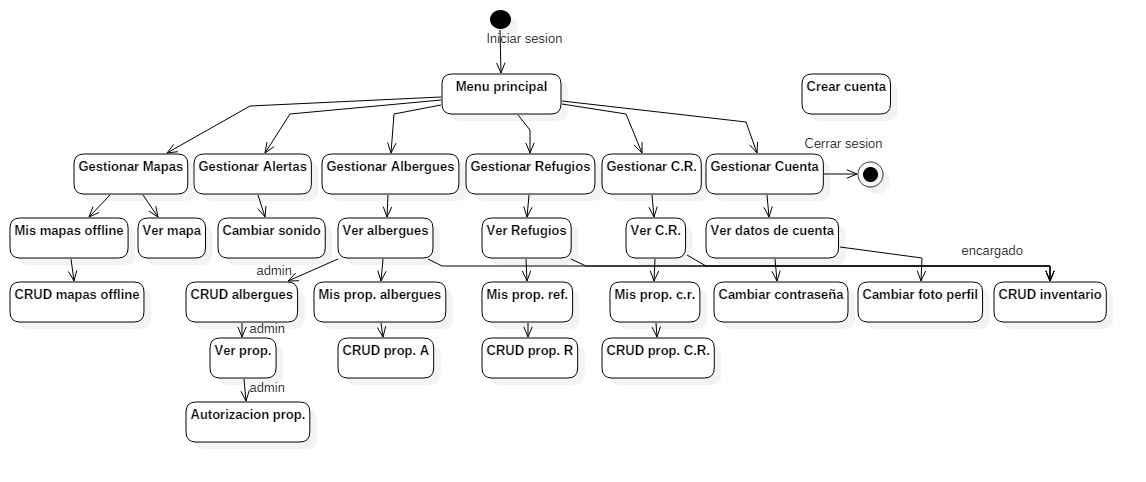
\includegraphics[width=1.2\textwidth]{images/NavDiagram}
		\caption{Diagrama de Navegación}
		\label{fig:NavDiagram}
	\end{center}
\end{figure}

	
	
	%Diseño de Interfaces
	%Se comenta para el reporte tecnico
	%\chapter{Diseño de Interfaces}
	%\label{chapter:interfaces}
	%%Entradas

%--------------------------------------
\section{IU01 Pantalla de Control de Acceso}

\subsection{Objetivo}
	Controlar el acceso al sistema mediante una contraseña a fin de que cada usuario acceda solo a las operaciones permitidas para su perfil.

\subsection{Diseño}
	Esta pantalla \IUref{IU01}{Pantalla de Control de Acceso} (ver figura~\ref{IU01}) aparece al iniciar el sistema. Para ingresar al mismo se debe escribir el usuario y la contraseña de acceso. 

\IUfig[.5]{IUs/IU01}{IU01}{Pantalla de Control de Acceso.}

\subsection{Salidas}

	Ninguna.

\subsection{Entradas}
Usuario y Contraseña del actor.

\subsection{Comandos}
\begin{itemize}
	\item \IUbutton{Iniciar Sesion}: Verifica que el usuario se encuentre registrado y la contraseña sea la correcta. Si la verificación es correcta identifica que tipo de usuario es y se muestra la \IUref{IU04}{Pantalla de Gestión de Alertas} (ver figura~\ref{IU04}) con sus respectivos permisos en la aplicación.
	\item \IUbutton{Crear Cuenta}: Muestra la \IUref{IU02}{Pantalla de creación de cuenta}.
\end{itemize}

\subsection{Mensajes}
\begin{Citemize}
	\item Usuario o contraseña incorrecta.
\end{Citemize}

\clearpage
%--------------------------------------
\section{IU02 Pantalla de creación de cuenta}

\subsection{Objetivo}
	Contar con un medio por el cual se pueda crear una nueva cuenta para el acceso al sistema.

\subsection{Diseño}
	Esta pantalla \IUref{IU02}{Pantalla de creacion de cuenta} (ver figura~\ref{fig:IU02}) aparece al oprimir \IUbutton{Crear Cuenta} desde la \IUref{IU01}{Pantalla de Control de Acceso} (ver figura~\ref{fig:IU01}). 
	
\IUfig[.5]{IUs/IU02}{IU02}{Pantalla de creación de cuenta.}

\subsection{Salidas}

	Ninguna.

\subsection{Entradas}
Usuario, correo electronico, nombre, apellidos, sexo, contraseña, repetir contraseña y fecha de nacimiento del Ciudadano.

\subsection{Comandos}
\begin{itemize}
	\item \IUbutton{Crear Cuenta}: Verifica que el usuario este disponible, que no falte ningun campo por llenar y que la contraseña sea igual en ambos casos. Si la verificación es correcta, se muestra la.. 
	\item \IUbutton{Cancelar}: Termina la operación y se muestra la \IUref{IU01}{Pantalla de Control de Acceso} (ver figura~\ref{fig:IU01}). 
\end{itemize}

\subsection{Mensajes}

\begin{Citemize}
	\item Usuario no disponible, intente con otro.
	\item La contraseña no coincide.
	\item Faltan campos por llenar.
\end{Citemize}




\clearpage
%--------------------------------------
\section{IU03 Pantalla de recuperacion de contraseña}

\subsection{Objetivo}
	Contar con un medio por el cual podamos recuperar nuestra contraseña en caso de olvidarla por medio de nuestro correo electronico.

\subsection{Diseño}
	Esta pantalla \IUref{IU03}{Pantalla de recuperación de contraseña} (ver figura~\ref{IU03}) aparece al oprimir \IUbutton{Recuperar contraseña}.

\IUfig[.5]{IUs/IU03}{IU03}{Pantalla de recuperacion de contraseña.}

\subsection{Salidas}

	Ninguna.

\subsection{Entradas}
Usuario o correo electronico con el que se registro la cuenta.

\subsection{Comandos}
\begin{itemize}
	\item \IUbutton{Enviar}: Verifica que el usuario o correo electronico pertenezca a alguna cuenta registrada en el sistema, si es asi muestra el mensaje - "La contraseña ah sido enviada a su correo electronico" y muestra la \IUref{IU01}{Pantalla de Control de Acceso} (ver figura~\ref{IU01}).
\end{itemize}

\subsection{Mensajes}

\begin{Citemize}
	\item El usuario no coincide con ninguna cuenta.
	\item El correo electronico no esta vinculado a ninguna cuenta.
	\item La contraseña ah sido enviada a su correo electronico
\end{Citemize}

\clearpage
%--------------------------------------
\section{IU04 Pantalla de Gestión de Alertas}

\subsection{Objetivo}
	Mostrar al usuario información acerca de los ultimos sismos registrados en la CDMX.

\subsection{Diseño}
	Esta pantalla \IUref{IU04}{Pantalla de Gestión de Alertas} (ver figura~\ref{IU04}) aparece al iniciar sesion. 

\IUfig[.5]{IUs/IU04}{IU04}{Pantalla de Gestión de Alertas.}

\subsection{Salidas}

	Historial de sismos detectados.

\subsection{Entradas}
	Ninguna.

\subsection{Comandos}
\begin{itemize}
	\item \IUbutton{Configurar alerta}: Muestra la \IUref{IU14}{Pantalla de Configuración de Alertas}.
	\item \IUbutton{Alertas}: Muestra la \IUref{IU04}{Pantalla de Selección de Seminario}.
	\item \IUbutton{Albergues}: Muestra la \IUref{IU05}{Pantalla de Gestión de Albergues}.
	\item \IUbutton{C.R.}: Muestra la \IUref{IU06}{Pantalla de Gestión de Centros de Recolección}.
	\item \IUbutton{Refugios}: Muestra la \IUref{IU07}{Pantalla de Gestión de Refugios}.
	\item \IUbutton{Mapas}: Muestra la \IUref{IU08}{Pantalla de Gestión de Mapas Offline}.
	\item \IUbutton{Cuenta}: Muestra la \IUref{IU09}{Pantalla de Gestión de Cuenta}.

\end{itemize}

\subsection{Mensajes}

\begin{Citemize}
	\item Sismo detectado.
\end{Citemize}

\clearpage
%--------------------------------------
\section{IU05 Pantalla de gestión de Albergues}

\subsection{Objetivo}
	Mostrar al Ciudadano información acerca de los albergues registrados en la CDMX y de proporcionar un medio rapido para su busqueda.

\subsection{Diseño}
	Esta pantalla \IUref{IU05}{Pantalla de gestión de Albergues} (ver figura~\ref{IU05}) aparece al oprimir \IUbutton{Albergues} ubicado en el Button Bar.

\IUfig[.5]{IUs/IU05}{IU05}{Pantalla de gestión de Albergues.}

\subsection{Salidas}

	Lista de Albergues autorizados.

\subsection{Entradas}
	Ninguna.

\subsection{Comandos}
\begin{itemize}
	\item \IUbutton{Mis propuestas de albergue}: Muestra la \IUref{IU10}{Pantalla de Gestión de Mis Propuestas de Albergue}.
	\item \IUbutton{Inventario}: Muestra la \IUref{IU13}{Pantalla de Inventario}.
	\item \IUbutton{Mapa}: Muestra la \IUref{IU08}{Pantalla de Gestión de Mapas Offline} mostrando el marcador del albergue seleccionado.
	\item \IUbutton{Alertas}: Muestra la \IUref{IU04}{Pantalla de Selección de Seminario}.
	\item \IUbutton{Albergues}: Muestra la \IUref{IU05}{Pantalla de Gestión de Albergues}.
	\item \IUbutton{C.R.}: Muestra la \IUref{IU06}{Pantalla de Gestión de Centros de Recolección}.
	\item \IUbutton{Refugios}: Muestra la \IUref{IU07}{Pantalla de Gestión de Refugios}.
	\item \IUbutton{Mapas}: Muestra la \IUref{IU08}{Pantalla de Gestión de Mapas Offline}.
	\item \IUbutton{Cuenta}: Muestra la \IUref{IU09}{Pantalla de Gestión de Cuenta}.
\end{itemize}

\subsection{Mensajes}

\begin{Citemize}
	\item Sin conexión a internet, los datos mostrados podrian no estar actualizados.
	\item Sin conexion a internet, no se cuenta con información acerca de los albergues.
\end{Citemize}

\clearpage
%--------------------------------------
\section{IU06 Pantalla de gestión de Centros de Recolección}

\subsection{Objetivo}
	Mostrar al Ciudadano información acerca de los centros de recolección registrados en la CDMX y de proporcionar un medio rapido para su busqueda.

\subsection{Diseño}
	Esta pantalla \IUref{IU06}{Pantalla de gestión de Centros de Recolección} (ver figura~\ref{IU06}) aparece al oprimir \IUbutton{C.R.} ubicado en el Button Bar.
	
\IUfig[.5]{IUs/IU06}{IU06}{Pantalla de gestión de Centros de Recolección.}

\subsection{Salidas}
	Lista de C.R. autorizados.

\subsection{Entradas}
	Ninguna.

\subsection{Comandos}
\begin{itemize}
	\item \IUbutton{Mis propuestas de C.R.}: Muestra la \IUref{IU11}{Pantalla de Gestión de Mis Propuestas de Centros de Recolección}.
	\item \IUbutton{Inventario}: Muestra la \IUref{IU13}{Pantalla de Inventario}.
	\item \IUbutton{Mapa}: Muestra la \IUref{IU08}{Pantalla de Gestión de Mapas} mostrando el marcador del albergue seleccionado.
	\item \IUbutton{Alertas}: Muestra la \IUref{IU04}{Pantalla de Selección de Seminario}.
	\item \IUbutton{Albergues}: Muestra la \IUref{IU05}{Pantalla de Gestión de Albergues}.
	\item \IUbutton{C.R.}: Muestra la \IUref{IU06}{Pantalla de Gestión de Centros de Recolección}.
	\item \IUbutton{Refugios}: Muestra la \IUref{IU07}{Pantalla de Gestión de Refugios}.
	\item \IUbutton{Mapas}: Muestra la \IUref{IU08}{Pantalla de Gestión de Mapas}.
	\item \IUbutton{Cuenta}: Muestra la \IUref{IU09}{Pantalla de Gestión de Cuenta}.
\end{itemize}

\subsection{Mensajes}

\begin{Citemize}
	\item Sin conexión a internet, los datos mostrados podrian no estar actualizados.
	\item Sin conexion a internet, no se cuenta con información acerca de los C.R.
\end{Citemize}

\clearpage
%--------------------------------------
\section{IU07 Pantalla de gestión de Refugios}

\subsection{Objetivo}
	Mostrar al Ciudadano información acerca de los refugios registrados en la CDMX y de proporcionar un medio rapido para su busqueda.

\subsection{Diseño}
	Esta pantalla \IUref{IU07}{Pantalla de gestión de Refugios} (ver figura~\ref{IU07}) aparece al oprimir \IUbutton{Refugios} ubicado en el Button Bar.
	
\IUfig[.5]{IUs/IU07}{IU07}{Pantalla de gestión de Refugios.}

\subsection{Salidas}

	Lista de Refugios autorizados.

\subsection{Entradas}
	Ninguna.

\subsection{Comandos}
\begin{itemize}
	\item \IUbutton{Mis propuestas de refugios}: Muestra la \IUref{IU12}{Pantalla de Gestión de Mis Propuestas de Refugios}.
	\item \IUbutton{Inventario}: Muestra la \IUref{IU13}{Pantalla de Inventario}.
	\item \IUbutton{Mapa}: Muestra la \IUref{IU08}{Pantalla de Gestión de Mapas} mostrando el marcador del albergue seleccionado.
	\item \IUbutton{Alertas}: Muestra la \IUref{IU04}{Pantalla de Selección de Seminario}.
	\item \IUbutton{Albergues}: Muestra la \IUref{IU05}{Pantalla de Gestión de Albergues}.
	\item \IUbutton{C.R.}: Muestra la \IUref{IU06}{Pantalla de Gestión de Centros de Recolección}.
	\item \IUbutton{Refugios}: Muestra la \IUref{IU07}{Pantalla de Gestión de Refugios}.
	\item \IUbutton{Mapas}: Muestra la \IUref{IU08}{Pantalla de Gestión de Mapas}.
	\item \IUbutton{Cuenta}: Muestra la \IUref{IU09}{Pantalla de Gestión de Cuenta}.
\end{itemize}

\subsection{Mensajes}

\begin{Citemize}
	\item Sin conexión a internet, los datos mostrados podrian no estar actualizados.
	\item Sin conexion a internet, no se cuenta con información acerca de los refugios.
\end{Citemize}

\clearpage
%--------------------------------------
\section{IU08 Pantalla de Gestión de Mapas}

\subsection{Objetivo}
	Permitir al Ciudadano visualizar mediante un Mapa la ubicación exacta de los Refugios, C.R. y Albergues registrados en la CDMX y de proporcionar un medio para mostrar una ruta a cualquiera de ellos.

\subsection{Diseño}
	Esta pantalla \IUref{IU08}{Pantalla de Gestión de Mapas} (ver figura~\ref{IU08}) aparece al oprimir \IUbutton{Mapas} ubicado en el Button Bar.
	
\IUfig[.5]{IUs/IU08}{IU08}{Pantalla de Gestión de Mapas.}

\subsection{Salidas}

	Ninguna.

\subsection{Entradas}
	Nombre o identificador del refugio, albergue o centros de recolección que se desee buscar.

\subsection{Comandos}
\begin{itemize}
	\item \IUbutton{Mis mapas offline}: Muestra la \IUref{IU15}{Pantalla de Gestión de Mis Mapas Offline}.
	\item \IUbutton{Search}: Muestra coincidencias de refugios, albergues o centros de recolección.
	\item \IUbutton{Mapa}: Muestra la \IUref{IU08}{Pantalla de Gestión de Mapas} mostrando el marcador del albergue seleccionado.
	\item \IUbutton{Alertas}: Muestra la \IUref{IU04}{Pantalla de Selección de Seminario}.
	\item \IUbutton{Albergues}: Muestra la \IUref{IU05}{Pantalla de Gestión de Albergues}.
	\item \IUbutton{C.R.}: Muestra la \IUref{IU06}{Pantalla de Gestión de Centros de Recolección}.
	\item \IUbutton{Refugios}: Muestra la \IUref{IU07}{Pantalla de Gestión de Refugios}.
	\item \IUbutton{Mapas}: Muestra la \IUref{IU08}{Pantalla de Gestión de Mapas}.
	\item \IUbutton{Cuenta}: Muestra la \IUref{IU09}{Pantalla de Gestión de Cuenta}.
\end{itemize}

\subsection{Mensajes}

\begin{Citemize}
	\item Error al conectar al servicio de mapas.
	\item Sin conexion a internet, se hara uso de sus mapas offline.
	\item No cuenta con ningun mapa offline descargado.
\end{Citemize}

\clearpage
%--------------------------------------
\section{IU09 Pantalla de Gestión de Cuenta}

\subsection{Objetivo}
	Permitir al Ciudadano gestionar datos de su cuenta y de proporcionar un medio para cerrar su sesion.

\subsection{Diseño}
	Esta pantalla \IUref{IU09}{Pantalla de Gestión de Cuenta} (ver figura~\ref{IU09}) aparece al oprimir \IUbutton{Cuenta} ubicado en el Button Bar.
	
\IUfig[.5]{IUs/IU09}{IU09}{Pantalla de Gestión de Cuenta.}

\subsection{Salidas}

	Lista de los mapas descargados anteriormente.

\subsection{Entradas}
	Ninguna.

\subsection{Comandos}
\begin{itemize}
	\item \IUbutton{Cerrar Sesion}: Termina nuestra sesion y muestra la \IUref{IU01}{Pantalla de Control de Acceso}.
	\item \IUbutton{Cambiar contraseña}: Permite cambiar nuestra actual contraseña por una nueva.
	\item \IUbutton{Cambiar foto de perfil}: Permite cambiar nuestra actual foto de perfil por una nueva.
	\item \IUbutton{Albergues}: Muestra la \IUref{IU05}{Pantalla de Gestión de Albergues}.
	\item \IUbutton{C.R.}: Muestra la \IUref{IU06}{Pantalla de Gestión de Centros de Recolección}.
	\item \IUbutton{Refugios}: Muestra la \IUref{IU07}{Pantalla de Gestión de Refugios}.
	\item \IUbutton{Mapas}: Muestra la \IUref{IU08}{Pantalla de Gestión de Mapas Offline}.
	\item \IUbutton{Cuenta}: Muestra la \IUref{IU09}{Pantalla de Gestión de Cuenta}.
\end{itemize}

\subsection{Mensajes}

	Ninguno.
%\begin{Citemize}
%	\item Error al verificar los datos de acceso, vuelva a intentarlo.
%\end{Citemize}

\clearpage
%--------------------------------------
\section{ IU10 Pantalla de Gestión de Mis Propuestas de Albergues}

\subsection{Objetivo}
	Mostrar al Ciudadano información acerca de sus propuestas de albergues, estatus de aceptacion/rechazo, de eliminarlas o modificarlas.

\subsection{Diseño}
	Esta pantalla \IUref{IU10}{Pantalla de Gestión de Mis Propuestas de Albergues} (ver figura~\ref{IU10}) aparece al oprimir \IUbutton{Mis propuestas de albergue} ubicado en la \IUref{IU05}{Pantalla de Gestión de Albergues}.
	
\IUfig[.5]{IUs/IU10}{IU10}{Pantalla de Gestión de Mis Propuestas de Albergues.}

\subsection{Salidas}
	Ninguna.

\subsection{Entradas}
	Ninguna.

\subsection{Comandos}
\begin{itemize}
	\item \IUbutton{Atras}: Muestra la \IUref{IU05}{Pantalla de Gestión de Albergues}.
	\item \IUbutton{Crear nueva prop.}: Muestra la \IUref{IU22}{Pantalla de Creación de una Propuesta de Albergue}.
	\item \IUbutton{Eliminar}: Muestra la \IUref{IU28}{Pantalla de Eliminación de Propuesta de Albergue}. 
	\item \IUbutton{Modificar}: Muestra la \IUref{IU26}{Pantalla de Modificación de una Propuesta de Albergue}.
	\item \IUbutton{Mapa}: Muestra la \IUref{IU08}{Pantalla de Gestión de Mapas} mostrando el marcador.
\end{itemize}

\subsection{Mensajes}

\begin{Citemize}
	\item No tiene registrada ninguna propuesta.
\end{Citemize}

\clearpage
%--------------------------------------
\section{IU11 Pantalla de Gestión de Mis Propuestas de Centros de Recolección}

\subsection{Objetivo}
	Mostrar al Ciudadano información acerca de sus propuestas de centros de recolección, estatus de aceptacion/rechazo, de eliminarlas o modificarlas.

\subsection{Diseño}
	Esta pantalla \IUref{IU11}{Pantalla de Gestión de Mis Propuestas de Albergues} (ver figura~\ref{IU11}) aparece al oprimir \IUbutton{Mis propuestas de C.R.} ubicado en la \IUref{IU06}{Pantalla de Gestión de Centros de Recolección}.
	
\IUfig[.5]{IUs/IU11}{IU11}{Pantalla de Gestión de Mis Propuestas de Centros de Recolección.}

\subsection{Salidas}

	Ninguna.

\subsection{Entradas}
	Ninguna.

\subsection{Comandos}
\begin{itemize}
	\item \IUbutton{Atras}: Muestra la \IUref{IU06}{Pantalla de Gestión de Centros de Recolección}.
	\item \IUbutton{Crear nueva prop.}: Muestra la \IUref{IU23}{Pantalla de Creación de una Propuesta de Centro de Recolección}.
	\item \IUbutton{Eliminar}: Muestra la \IUref{IU29}{Pantalla de Eliminación de Propuesta de Centro de Recolección}. 
	\item \IUbutton{Modificar}: Muestra la \IUref{IU27}{Pantalla de Modificación de una Propuesta de Centro de Recolección}.
	\item \IUbutton{Mapa}: Muestra la \IUref{IU08}{Pantalla de Gestión de Mapas} mostrando el marcador.
\end{itemize}

\subsection{Mensajes}

\begin{Citemize}
	\item No tiene registrada ninguna propuesta.
\end{Citemize}

\clearpage
%--------------------------------------
\section{IU12 Pantalla de Gestión de Mis Propuestas de Refugios}

\subsection{Objetivo}
	Mostrar al Ciudadano información acerca de sus propuestas de centros de recolección, estatus de aceptacion/rechazo, de eliminarlas, modificarlas y crear nuevas.

\subsection{Diseño}
	Esta pantalla \IUref{IU12}{Pantalla de Gestión de Mis Propuestas de Refugios} (ver figura~\ref{IU12}) aparece al oprimir \IUbutton{Mis propuestas de Refugios} ubicado en la \IUref{IU07}{Pantalla de Gestión de Refugios}.
	
\IUfig[.5]{IUs/IU12}{IU12}{Pantalla de Gestión de Mis Propuestas de Refugios.}

\subsection{Salidas}

	Ninguna.

\subsection{Entradas}
	Ninguna.

\subsection{Comandos}
\begin{itemize}
	\item \IUbutton{Atras}: Muestra la \IUref{IU07}{Pantalla de Gestión de Refugios}.
	\item \IUbutton{Crear nueva prop.}: Muestra la \IUref{IU24}{Pantalla de Creación de una Propuesta de Refugio}.
	\item \IUbutton{Eliminar}: Muestra la \IUref{IU30}{Pantalla de Eliminación de Propuesta de Refugio}. 
	\item \IUbutton{Modificar}: Muestra la \IUref{IU25}{Pantalla de Modificación de una Propuesta de Refugio}.
	\item \IUbutton{Mapa}: Muestra la \IUref{IU08}{Pantalla de Gestión de Mapas} mostrando el marcador.
\end{itemize}

\subsection{Mensajes}

\begin{Citemize}
	\item No tiene registrada ninguna propuesta.
\end{Citemize}

\clearpage
%--------------------------------------
\section{IU13 Pantalla de Inventario}

\subsection{Objetivo}
	Mostrar al Ciudadano un inventario con todos los articulos y herramientas disponibles en el refugio, centro de recolección o albergue al que pertenezca, asi como un nivel de importancia el cual podra servir como referencia a la hora de hacer una donación al lugar.

\subsection{Diseño}
	Esta pantalla \IUref{IU13}{Pantalla de Inventario} (ver figura~\ref{IU13}) aparece al oprimir \IUbutton{Inventario} ubicado en la \IUref{IU05}{Pantalla de Gestión de Albergues}, \IUref{IU06}{Pantalla de Gestión de C.R.} o \IUref{IU07}{Pantalla de Gestión de Refugios} segun sea el caso.
	
\IUfig[.5]{IUs/IU13}{IU13}{Pantalla de Inventario.}

\subsection{Salidas}

	Inventario.

\subsection{Entradas}
	Identificador del refugio, centro de recolección o albergue mediante la seleccion del mismo.

\subsection{Comandos}
\begin{itemize}
	\item \IUbutton{Atras}: Muestra la \IUref{IU05}{Pantalla de Gestión de Albergues}, \IUref{IU06}{Pantalla de Gestión de C.R.} o \IUref{IU07}{Pantalla de Gestión de Refugios} segun sea el caso.
\end{itemize}

\subsection{Mensajes}

\begin{Citemize}
	\item Sin conexión a internet, los datos mostrados podrian no estar actualizados.
	\item Sin conexion a internet, no se cuenta con información acerca del inventario.
\end{Citemize}

\clearpage
%--------------------------------------
\section{IU14 Pantalla de configuración de alertas}

\subsection{Objetivo}
	Proporcionar al Ciudadano un medio por el cual pueda cambiar el sonido predeterminado de una alerta en caso de sismo por uno de su preferencia.

\subsection{Diseño}
	Esta pantalla \IUref{IU14}{Pantalla de configuración de alertas} (ver figura~\ref{IU14}) aparece al oprimir \IUbutton{Config. alerta} ubicado en la \IUref{IU04}{Pantalla de Gestión de Alertas}.
	
\IUfig[.5]{IUs/IU14}{IU14}{Pantalla de configuración de alertas.}

\subsection{Salidas}

	Ninguna.

\subsection{Entradas}
	Sonido del repertorio.

\subsection{Comandos}
\begin{itemize}
	\item \IUbutton{Cambiar sonido de alerta}: Guarda el nuevo sonido de alerta seleccionado.
	\item \IUbutton{Atras}: Muestra la \IUref{IU04}{Pantalla de Gestión de Alertas}.
\end{itemize}

\subsection{Mensajes}

\begin{Citemize}
	\item Ah cambiado el sonido de la alerta.
	\item Error al cambiar el sonido de alerta, intentelo de nuevo.
\end{Citemize}

\clearpage
%--------------------------------------
\section{IU15 Pantalla de Gestión de Mis Mapas Offline}

\subsection{Objetivo}
	Mostrar al Ciudadano información acerca de sus mapas descargados, de eliminarlos, de modificarlos y de descargar nuevos.

\subsection{Diseño}
	Esta pantalla \IUref{IU15}{Pantalla de Gestión de Mis Mapas Offline} (ver figura~\ref{IU15}) aparece al oprimir \IUbutton{Mis mapas offline} ubicado en la \IUref{IU08}{Pantalla de Gestión de Mapas}.
	
\IUfig[.5]{IUs/IU15}{IU15}{Pantalla de Gestión de Mis Mapas Offline.}

\subsection{Salidas}

	Ninguna.

\subsection{Entradas}
	Ninguna.

\subsection{Comandos}
\begin{itemize}
	\item \IUbutton{Mapa}: Muestra la \IUref{IU16}{Pantalla de Control de un Mapa Offline} con los datos del mapa offline seleccionado.
	\item \IUbutton{Atras}: Muestra la \IUref{IU008}{Pantalla de Gestión de Mapas}.
\end{itemize}

\subsection{Mensajes}

\begin{Citemize}
	\item No tiene ningun mapa descargado.
\end{Citemize}

\clearpage
%--------------------------------------
\section{IU16 Pantalla de control de un Mapa Offline}

\subsection{Objetivo}
	Controlar el acceso al sistema mediante una contraseña a fin de que cada usuario acceda solo a las operaciones permitidas para su perfil.

\subsection{Diseño}
	Esta pantalla .. aparece al iniciar el sistema. Para ingresar al mismo se debe escribir el Número de Boleta del estudiante y la contraseña de acceso. 
%\IUref{IU23}{Pantalla de Control de Acceso} (ver figura~\ref{IU23})
\IUfig[.5]{IUs/IU16}{IU16}{Pantalla de control de un Mapa Offline.}

\subsection{Salidas}

	Ninguna.

\subsection{Entradas}
Número de Boleta y Contraseña del Estudiante.

\subsection{Comandos}
\begin{itemize}
	\item \IUbutton{Entrar}: Verifica que el Estudiante se encuentre registrado y la contraseña sea la correcta. Si la verificación es correcta, se muestra la ...
	\item \IUbutton{Ayuda}: Muestra la ayuda de esta pantalla %\IUref{IU50}{Pantalla de Ayuda}.
	%\IUref{UI32}{Pantalla de Selección de Seminario}.
\end{itemize}

\subsection{Mensajes}

\begin{Citemize}
	\item Error al verificar los datos de acceso, vuelva a intentarlo.
\end{Citemize}

\clearpage
%--------------------------------------
\section{IU17 Pantalla de Borrado de un Mapa Offline}

\subsection{Objetivo}
	Controlar el acceso al sistema mediante una contraseña a fin de que cada usuario acceda solo a las operaciones permitidas para su perfil.

\subsection{Diseño}
	Esta pantalla .. aparece al iniciar el sistema. Para ingresar al mismo se debe escribir el Número de Boleta del estudiante y la contraseña de acceso. 
%\IUref{IU23}{Pantalla de Control de Acceso} (ver figura~\ref{IU23})
\IUfig[.5]{IUs/IU17}{IU17}{Pantalla de Borrado de un Mapa Offline.}

\subsection{Salidas}

	Ninguna.

\subsection{Entradas}
Número de Boleta y Contraseña del Estudiante.

\subsection{Comandos}
\begin{itemize}
	\item \IUbutton{Entrar}: Verifica que el Estudiante se encuentre registrado y la contraseña sea la correcta. Si la verificación es correcta, se muestra la ...
	\item \IUbutton{Ayuda}: Muestra la ayuda de esta pantalla %\IUref{IU50}{Pantalla de Ayuda}.
	%\IUref{UI32}{Pantalla de Selección de Seminario}.
\end{itemize}

\subsection{Mensajes}

\begin{Citemize}
	\item Error al verificar los datos de acceso, vuelva a intentarlo.
\end{Citemize}

\clearpage
%--------------------------------------
\section{IU18 Pantalla de Actualización de Mapa Oflline}

\subsection{Objetivo}
	Controlar el acceso al sistema mediante una contraseña a fin de que cada usuario acceda solo a las operaciones permitidas para su perfil.

\subsection{Diseño}
	Esta pantalla .. aparece al iniciar el sistema. Para ingresar al mismo se debe escribir el Número de Boleta del estudiante y la contraseña de acceso. 
%\IUref{IU23}{Pantalla de Control de Acceso} (ver figura~\ref{IU23})
\IUfig[.5]{IUs/IU18}{IU18}{Pantalla de Actualización de Mapa Oflline.}

\subsection{Salidas}

	Ninguna.

\subsection{Entradas}
Número de Boleta y Contraseña del Estudiante.

\subsection{Comandos}
\begin{itemize}
	\item \IUbutton{Entrar}: Verifica que el Estudiante se encuentre registrado y la contraseña sea la correcta. Si la verificación es correcta, se muestra la ...
	\item \IUbutton{Ayuda}: Muestra la ayuda de esta pantalla %\IUref{IU50}{Pantalla de Ayuda}.
	%\IUref{UI32}{Pantalla de Selección de Seminario}.
\end{itemize}

\subsection{Mensajes}

\begin{Citemize}
	\item Error al verificar los datos de acceso, vuelva a intentarlo.
\end{Citemize}

\clearpage
%--------------------------------------
\section{IU19 Pantalla de Descarga de un Mapa Offline}

\subsection{Objetivo}
	Controlar el acceso al sistema mediante una contraseña a fin de que cada usuario acceda solo a las operaciones permitidas para su perfil.

\subsection{Diseño}
	Esta pantalla .. aparece al iniciar el sistema. Para ingresar al mismo se debe escribir el Número de Boleta del estudiante y la contraseña de acceso. 
%\IUref{IU23}{Pantalla de Control de Acceso} (ver figura~\ref{IU23})
\IUfig[.5]{IUs/IU19}{IU19}{Pantalla de Descarga de un Mapa Offline.}

\subsection{Salidas}

	Ninguna.

\subsection{Entradas}
Número de Boleta y Contraseña del Estudiante.

\subsection{Comandos}
\begin{itemize}
	\item \IUbutton{Entrar}: Verifica que el Estudiante se encuentre registrado y la contraseña sea la correcta. Si la verificación es correcta, se muestra la ...
	\item \IUbutton{Ayuda}: Muestra la ayuda de esta pantalla %\IUref{IU50}{Pantalla de Ayuda}.
	%\IUref{UI32}{Pantalla de Selección de Seminario}.
\end{itemize}

\subsection{Mensajes}

\begin{Citemize}
	\item Error al verificar los datos de acceso, vuelva a intentarlo.
\end{Citemize}

\clearpage
%--------------------------------------
\section{IU20 Pantalla de Proceso de Descaraga de un Mapa Offline}

\subsection{Objetivo}
	Controlar el acceso al sistema mediante una contraseña a fin de que cada usuario acceda solo a las operaciones permitidas para su perfil.

\subsection{Diseño}
	Esta pantalla .. aparece al iniciar el sistema. Para ingresar al mismo se debe escribir el Número de Boleta del estudiante y la contraseña de acceso. 
%\IUref{IU23}{Pantalla de Control de Acceso} (ver figura~\ref{IU23})
\IUfig[.5]{IUs/IU20}{IU20}{Pantalla de Proceso de Descaraga de un Mapa Offline.}

\subsection{Salidas}

	Ninguna.

\subsection{Entradas}
Número de Boleta y Contraseña del Estudiante.

\subsection{Comandos}
\begin{itemize}
	\item \IUbutton{Entrar}: Verifica que el Estudiante se encuentre registrado y la contraseña sea la correcta. Si la verificación es correcta, se muestra la ...
	\item \IUbutton{Ayuda}: Muestra la ayuda de esta pantalla %\IUref{IU50}{Pantalla de Ayuda}.
	%\IUref{UI32}{Pantalla de Selección de Seminario}.
\end{itemize}

\subsection{Mensajes}

\begin{Citemize}
	\item Error al verificar los datos de acceso, vuelva a intentarlo.
\end{Citemize}

\clearpage
%--------------------------------------
\section{IU21 Pantalla de Modificación de Nombre de un Mapa Offline}

\subsection{Objetivo}
	Controlar el acceso al sistema mediante una contraseña a fin de que cada usuario acceda solo a las operaciones permitidas para su perfil.

\subsection{Diseño}
	Esta pantalla .. aparece al iniciar el sistema. Para ingresar al mismo se debe escribir el Número de Boleta del estudiante y la contraseña de acceso. 
%\IUref{IU23}{Pantalla de Control de Acceso} (ver figura~\ref{IU23})
\IUfig[.5]{IUs/IU21}{IU21}{Pantalla de Modificación de Nombre de un Mapa Offline.}

\subsection{Salidas}

	Ninguna.

\subsection{Entradas}
Número de Boleta y Contraseña del Estudiante.

\subsection{Comandos}
\begin{itemize}
	\item \IUbutton{Entrar}: Verifica que el Estudiante se encuentre registrado y la contraseña sea la correcta. Si la verificación es correcta, se muestra la ...
	\item \IUbutton{Ayuda}: Muestra la ayuda de esta pantalla %\IUref{IU50}{Pantalla de Ayuda}.
	%\IUref{UI32}{Pantalla de Selección de Seminario}.
\end{itemize}

\subsection{Mensajes}

\begin{Citemize}
	\item Error al verificar los datos de acceso, vuelva a intentarlo.
\end{Citemize}

\clearpage
%--------------------------------------
\section{IU22 Pantalla de Creación de una Propuesta de Albergue}

\subsection{Objetivo}
	Controlar el acceso al sistema mediante una contraseña a fin de que cada usuario acceda solo a las operaciones permitidas para su perfil.

\subsection{Diseño}
	Esta pantalla .. aparece al iniciar el sistema. Para ingresar al mismo se debe escribir el Número de Boleta del estudiante y la contraseña de acceso. 
%\IUref{IU23}{Pantalla de Control de Acceso} (ver figura~\ref{IU23})
\IUfig[.5]{IUs/IU22}{IU22}{Pantalla de Creación de una Propuesta de Albergue.}

\subsection{Salidas}

	Ninguna.

\subsection{Entradas}
Número de Boleta y Contraseña del Estudiante.

\subsection{Comandos}
\begin{itemize}
	\item \IUbutton{Entrar}: Verifica que el Estudiante se encuentre registrado y la contraseña sea la correcta. Si la verificación es correcta, se muestra la ...
	\item \IUbutton{Ayuda}: Muestra la ayuda de esta pantalla %\IUref{IU50}{Pantalla de Ayuda}.
	%\IUref{UI32}{Pantalla de Selección de Seminario}.
\end{itemize}

\subsection{Mensajes}

\begin{Citemize}
	\item Error al verificar los datos de acceso, vuelva a intentarlo.
\end{Citemize}

\clearpage
%--------------------------------------
\section{IU23 Pantalla de Creación de una Propuesta de Centro de Recolección}

\subsection{Objetivo}
	Controlar el acceso al sistema mediante una contraseña a fin de que cada usuario acceda solo a las operaciones permitidas para su perfil.

\subsection{Diseño}
	Esta pantalla .. aparece al iniciar el sistema. Para ingresar al mismo se debe escribir el Número de Boleta del estudiante y la contraseña de acceso. 
%\IUref{IU23}{Pantalla de Control de Acceso} (ver figura~\ref{IU23})
\IUfig[.5]{IUs/IU23}{IU23}{Pantalla de Creación de una Propuesta de Centro de Recolección.}

\subsection{Salidas}

	Ninguna.

\subsection{Entradas}
Número de Boleta y Contraseña del Estudiante.

\subsection{Comandos}
\begin{itemize}
	\item \IUbutton{Entrar}: Verifica que el Estudiante se encuentre registrado y la contraseña sea la correcta. Si la verificación es correcta, se muestra la ...
	\item \IUbutton{Ayuda}: Muestra la ayuda de esta pantalla %\IUref{IU50}{Pantalla de Ayuda}.
	%\IUref{UI32}{Pantalla de Selección de Seminario}.
\end{itemize}

\subsection{Mensajes}

\begin{Citemize}
	\item Error al verificar los datos de acceso, vuelva a intentarlo.
\end{Citemize}

\clearpage
%--------------------------------------
\section{IU24 Pantalla de Creación de una Propuesta de Refugio}

\subsection{Objetivo}
	Controlar el acceso al sistema mediante una contraseña a fin de que cada usuario acceda solo a las operaciones permitidas para su perfil.

\subsection{Diseño}
	Esta pantalla .. aparece al iniciar el sistema. Para ingresar al mismo se debe escribir el Número de Boleta del estudiante y la contraseña de acceso. 
%\IUref{IU23}{Pantalla de Control de Acceso} (ver figura~\ref{IU23})
\IUfig[.5]{IUs/IU24}{IU24}{Pantalla de Creación de una Propuesta de Refugio.}
\subsection{Salidas}

	Ninguna.

\subsection{Entradas}
Número de Boleta y Contraseña del Estudiante.

\subsection{Comandos}
\begin{itemize}
	\item \IUbutton{Entrar}: Verifica que el Estudiante se encuentre registrado y la contraseña sea la correcta. Si la verificación es correcta, se muestra la ...
	\item \IUbutton{Ayuda}: Muestra la ayuda de esta pantalla %\IUref{IU50}{Pantalla de Ayuda}.
	%\IUref{UI32}{Pantalla de Selección de Seminario}.
\end{itemize}

\subsection{Mensajes}

\begin{Citemize}
	\item Error al verificar los datos de acceso, vuelva a intentarlo.
\end{Citemize}

\clearpage
%--------------------------------------
\section{IU25 Pantalla de Modificación de Propuesta de Refugio}

\subsection{Objetivo}
	Controlar el acceso al sistema mediante una contraseña a fin de que cada usuario acceda solo a las operaciones permitidas para su perfil.

\subsection{Diseño}
	Esta pantalla .. aparece al iniciar el sistema. Para ingresar al mismo se debe escribir el Número de Boleta del estudiante y la contraseña de acceso. 
%\IUref{IU23}{Pantalla de Control de Acceso} (ver figura~\ref{IU23})
\IUfig[.5]{IUs/IU25}{IU25}{Pantalla de Modificación de Propuesta de Refugio.}

\subsection{Salidas}

	Ninguna.

\subsection{Entradas}
Número de Boleta y Contraseña del Estudiante.

\subsection{Comandos}
\begin{itemize}
	\item \IUbutton{Entrar}: Verifica que el Estudiante se encuentre registrado y la contraseña sea la correcta. Si la verificación es correcta, se muestra la ...
	\item \IUbutton{Ayuda}: Muestra la ayuda de esta pantalla %\IUref{IU50}{Pantalla de Ayuda}.
	%\IUref{UI32}{Pantalla de Selección de Seminario}.
\end{itemize}

\subsection{Mensajes}

\begin{Citemize}
	\item Error al verificar los datos de acceso, vuelva a intentarlo.
\end{Citemize}

\clearpage
%--------------------------------------
\section{IU26 Pantalla de Modificación de Propuesta de Albergue}

\subsection{Objetivo}
	Controlar el acceso al sistema mediante una contraseña a fin de que cada usuario acceda solo a las operaciones permitidas para su perfil.

\subsection{Diseño}
	Esta pantalla .. aparece al iniciar el sistema. Para ingresar al mismo se debe escribir el Número de Boleta del estudiante y la contraseña de acceso. 
%\IUref{IU23}{Pantalla de Control de Acceso} (ver figura~\ref{IU23})
\IUfig[.5]{IUs/IU26}{IU26}{Pantalla de Modificación de Propuesta de Albergue.}

\subsection{Salidas}

	Ninguna.

\subsection{Entradas}
Número de Boleta y Contraseña del Estudiante.

\subsection{Comandos}
\begin{itemize}
	\item \IUbutton{Entrar}: Verifica que el Estudiante se encuentre registrado y la contraseña sea la correcta. Si la verificación es correcta, se muestra la ...
	\item \IUbutton{Ayuda}: Muestra la ayuda de esta pantalla %\IUref{IU50}{Pantalla de Ayuda}.
	%\IUref{UI32}{Pantalla de Selección de Seminario}.
\end{itemize}

\subsection{Mensajes}

\begin{Citemize}
	\item Error al verificar los datos de acceso, vuelva a intentarlo.
\end{Citemize}

\clearpage
%--------------------------------------
\section{IU27 Pantalla de Modificación de Propuesta de Centro de Recolección}

\subsection{Objetivo}
	Controlar el acceso al sistema mediante una contraseña a fin de que cada usuario acceda solo a las operaciones permitidas para su perfil.

\subsection{Diseño}
	Esta pantalla .. aparece al iniciar el sistema. Para ingresar al mismo se debe escribir el Número de Boleta del estudiante y la contraseña de acceso. 
%\IUref{IU23}{Pantalla de Control de Acceso} (ver figura~\ref{IU23})
\IUfig[.5]{IUs/IU27}{IU27}{Pantalla de Modificación de Propuesta de Centro de Recolección.}

\subsection{Salidas}

	Ninguna.

\subsection{Entradas}
Número de Boleta y Contraseña del Estudiante.

\subsection{Comandos}
\begin{itemize}
	\item \IUbutton{Entrar}: Verifica que el Estudiante se encuentre registrado y la contraseña sea la correcta. Si la verificación es correcta, se muestra la ...
	\item \IUbutton{Ayuda}: Muestra la ayuda de esta pantalla %\IUref{IU50}{Pantalla de Ayuda}.
	%\IUref{UI32}{Pantalla de Selección de Seminario}.
\end{itemize}

\subsection{Mensajes}

\begin{Citemize}
	\item Error al verificar los datos de acceso, vuelva a intentarlo.
\end{Citemize}

\clearpage
%--------------------------------------
\section{IU28 Pantalla de Eliminación de Propuesta de Albergue}

\subsection{Objetivo}
	Controlar el acceso al sistema mediante una contraseña a fin de que cada usuario acceda solo a las operaciones permitidas para su perfil.

\subsection{Diseño}
	Esta pantalla .. aparece al iniciar el sistema. Para ingresar al mismo se debe escribir el Número de Boleta del estudiante y la contraseña de acceso. 
%\IUref{IU23}{Pantalla de Control de Acceso} (ver figura~\ref{IU23})
\IUfig[.5]{IUs/IU28}{IU28}{Pantalla de Eliminación de Propuesta de Albergue.}

\subsection{Salidas}

	Ninguna.

\subsection{Entradas}
Número de Boleta y Contraseña del Estudiante.

\subsection{Comandos}
\begin{itemize}
	\item \IUbutton{Entrar}: Verifica que el Estudiante se encuentre registrado y la contraseña sea la correcta. Si la verificación es correcta, se muestra la ...
	\item \IUbutton{Ayuda}: Muestra la ayuda de esta pantalla %\IUref{IU50}{Pantalla de Ayuda}.
	%\IUref{UI32}{Pantalla de Selección de Seminario}.
\end{itemize}

\subsection{Mensajes}

\begin{Citemize}
	\item Error al verificar los datos de acceso, vuelva a intentarlo.
\end{Citemize}

\clearpage
%--------------------------------------
\section{IU29 Pantalla de Eliminación de Propuesta de Centro de Recolección}

\subsection{Objetivo}
	Controlar el acceso al sistema mediante una contraseña a fin de que cada usuario acceda solo a las operaciones permitidas para su perfil.

\subsection{Diseño}
	Esta pantalla .. aparece al iniciar el sistema. Para ingresar al mismo se debe escribir el Número de Boleta del estudiante y la contraseña de acceso. 
%\IUref{IU23}{Pantalla de Control de Acceso} (ver figura~\ref{IU23})
\IUfig[.5]{IUs/IU29}{IU29}{Pantalla de Eliminación de Propuesta de Centro de Recolección.}

\subsection{Salidas}

	Ninguna.

\subsection{Entradas}
Número de Boleta y Contraseña del Estudiante.

\subsection{Comandos}
\begin{itemize}
	\item \IUbutton{Entrar}: Verifica que el Estudiante se encuentre registrado y la contraseña sea la correcta. Si la verificación es correcta, se muestra la ...
	\item \IUbutton{Ayuda}: Muestra la ayuda de esta pantalla %\IUref{IU50}{Pantalla de Ayuda}.
	%\IUref{UI32}{Pantalla de Selección de Seminario}.
\end{itemize}

\subsection{Mensajes}

\begin{Citemize}
	\item Error al verificar los datos de acceso, vuelva a intentarlo.
\end{Citemize}

\clearpage
%--------------------------------------
\section{IU30 Pantalla de Eliminación de Propuesta de Refugio}

\subsection{Objetivo}
	Controlar el acceso al sistema mediante una contraseña a fin de que cada usuario acceda solo a las operaciones permitidas para su perfil.

\subsection{Diseño}
	Esta pantalla .. aparece al iniciar el sistema. Para ingresar al mismo se debe escribir el Número de Boleta del estudiante y la contraseña de acceso. 
%\IUref{IU23}{Pantalla de Control de Acceso} (ver figura~\ref{IU23})
\IUfig[.5]{IUs/IU30}{IU30}{Pantalla de Eliminación de Propuesta de Refugio.}

\subsection{Salidas}

	Ninguna.

\subsection{Entradas}
Número de Boleta y Contraseña del Estudiante.

\subsection{Comandos}
\begin{itemize}
	\item \IUbutton{Entrar}: Verifica que el Estudiante se encuentre registrado y la contraseña sea la correcta. Si la verificación es correcta, se muestra la ...
	\item \IUbutton{Ayuda}: Muestra la ayuda de esta pantalla %\IUref{IU50}{Pantalla de Ayuda}.
	%\IUref{UI32}{Pantalla de Selección de Seminario}.
\end{itemize}

\subsection{Mensajes}

\begin{Citemize}
	\item Error al verificar los datos de acceso, vuelva a intentarlo.
\end{Citemize}

\clearpage

	
	%Falta definir entorno mensajes
	%Se comenta para el reporte tecnico
	%\chapter{Diseño de Mensajes}
	%\label{chapter:msgs}
	%\chapter{Mensajes del sistema}
%\label{chapter:mensajes}
\cdtLabel{apendice:Mensajes}{}


%===========================  MSG1 ==================================
\begin{mensaje}{MSG1}{Campos sin llenar}{Error \msgError}
	\item[Canal:] Sistema
    \item[Propósito:] Alertar al actor que ingreso sus datos en el sistema.
    \item[Redacción:] ¡No hay $<DATOS>$ para ingresar!
    \item[Parámetros:] DATOS: Información de la cual se requiere para Iniciar Sesion y concluir un proceso
    \item[Ejemplo:] ¡hay campos sin llenar!
\end{mensaje}
%============================== MSG2 =================================
\begin{mensaje}{MSG2}{Usuario ya existente }{Error \msgError}
	\item[Canal:] Sistema
    \item[Propósito:] Alertar al actor que el Nombre de Usuario que se desea ya está disponible en el sistema.
    \item[Redacción:] ¡Este/a $<USUARIO>$ ya esta disponible !
    \item[Parámetros:] Usuario:Información de un registro en específico de la cual se requiere para concluir un proceso.
    \item[Ejemplo:] ¡el usuario ya esta en uso!
\end{mensaje}
%============================== MSG3 =================================
\begin{mensaje}{MSG3}{Contraseña Incorrecta}{Error \msgError}
	\item[Canal:] Sistema
    \item[Propósito:] Alertar al actor que la Contraseña  que se Ingreso es incorrecta.
    \item[Redacción:] ¡Este/a $<CONTRASENA>$ es inocrrecta!
    \item[Parámetros:] Contraseña:Información de un registro en específico de la cual se requiere para concluir un proceso.
    \item[Ejemplo:] ¡contraseña incorrecta!
\end{mensaje}
%============================== MSG4 =================================
\begin{mensaje}{MSG4}{Sin conexión a Internet }{Notificación \msgNotif}
	\item[Canal:] Sistema
    \item[Propósito:] Alertar al actor que no tiene acceso a internet.
    \item[Redacción:] ¡El sistema esta $<SIN CONEXION>$ a Internet !
    \item[Parámetros:] Sin Conexión:Notificación que es necesaria para llevar a cabo un Ingreso.
    \item[Ejemplo:] ¡sin conexión a internet!
\end{mensaje}
%============================== MSG5 =================================
\begin{mensaje}{MSG5}{Nombre de Usuario o Contraeña incorrecto }{Error \msgError}
	\item[Canal:] Sistema
    \item[Propósito:] Alertar al actor que el Nombre de Usuario o Contraseña que se ingreso es incorrecto en el sistema.
    \item[Redacción:] ¡Este/a $<USUARIO>$ o $<CONTRASENA>$ es incorrecto !
    \item[Parámetros:] Usuario y Contraseña :Información de un registro en específico de la cual se requiere para concluir un proceso.
    \item[Ejemplo:] ¡usuario o contraseña son incorrectos!
\end{mensaje}
%============================== MSG6 =================================
\begin{mensaje}{MSG6}{La Contraseña no coinciden }{Error \msgError}
	\item[Canal:] Sistema
    \item[Propósito:] Alertar al actor que sus contraseñas que ingreso no coinciden para el sistema.
    \item[Redacción:] ¡Este/a $<CONTRASENA>$ no son las mismas !
    \item[Parámetros:] Usuario:Información de un registro en específico de la cual se requiere para concluir un proceso.
    \item[Ejemplo:] ¡las contraseñas no coinciden!
\end{mensaje}
%============================== MSG7 =================================
\begin{mensaje}{MSG6}{Recupero Contraseña }{Notificación \msgNotif}
	\item[Canal:] Sistema
    \item[Propósito:] Informar al actor que la operacion se llevo a cabo exitosamente.
    \item[Redacción:] ¡Este/a $<OPERACION>$ no son las mismas !
    \item[Parámetros:] OPERACION:Actividad que el actor debe realizar
    \item[Ejemplo:] ¡se recupero la contraseña correctamente!
\end{mensaje}
%===========================  MSG8 ==================================
\begin{mensaje}{MSG8}{Modificación Exitosa}{Confirmación \msgConfirm}
	\item[Canal:] Sistema
    \item[Propósito:] Informar al actor que la operación que se le ha solicitado al sistema se llevo a cabo exitosamente.
    \item[Redacción:] El $<MODIFICAR>$ se llevo a cabo correctamente.
    \item[Parámetros:] Modificar: Actividad que el actor debe realizar.
    \item[Ejemplo:] ¡la modificación se llevo a cabo correctamente!
\end{mensaje}
%===========================  MSG9 ==================================
\begin{mensaje}{MSG9}{Eliminación Exitosa}{Confirmación \msgConfirm}
	\item[Canal:] Sistema
    \item[Propósito:] Informar al actor que la operación que se le ha solicitado al sistema se llevo a cabo exitosamente.
    \item[Redacción:] El $<ELIMINAR>$ se llevo a cabo correctamente.
    \item[Parámetros:] ELIMINAR: Actividad que el actor debe realizar.
    \item[Ejemplo:]¡elimiación correcta!
\end{mensaje}
%===========================  MSG10 ==================================
\begin{mensaje}{MSG10}{Registro Existoso}{Confirmación \msgConfirm}
	\item[Canal:] Sistema
    \item[Propósito:] Informar al actor que la operación que se le ha solicitado al sistema se llevo a cabo exitosamente.
    \item[Redacción:] El $<REGISTRO>$ se llevo a cabo correctamente.
    \item[Parámetros:] REGISTRO: Actividad que el actor debe realizar.
    \item[Ejemplo:] ¡registro correcto!
\end{mensaje}
%===========================  MSG11 ==================================
\begin{mensaje}{MSG11}{Autorizacion Exitosa}{Confirmación \msgConfirm}
	\item[Canal:] Sistema
    \item[Propósito:] Informar al actor que la operación que se le ha solicitado al sistema se llevo a cabo exitosamente.
    \item[Redacción:] La $<AUTORIZACION>$ se llevo a cabo correctamente.
    \item[Parámetros:] OPERACION: Actividad que el actor debe realizar.
    \item[Ejemplo:] ¡Autorización validada!
\end{mensaje}
%===========================  MSG12 ==================================
\begin{mensaje}{MSG12}{Autorizacion Rechazada}{Error \msgError}
	\item[Canal:] Sistema
    \item[Propósito:] Informar al actor que la operación que se le ha solicitado no se llevo a cabo exitosamente.
    \item[Redacción:] La $<AUTORIZACION>$ No se llevo a cabo correctamente.
    \item[Parámetros:] OPERACION: Actividad que el actor debe realizar.
    \item[Ejemplo:] ¡autorización invalida
\end{mensaje}
%===========================  MSG13 ==================================
\begin{mensaje}{MSG13}{Propuesta Registrada}{Confirmación \msgConfirm}
	\item[Canal:] Sistema
    \item[Propósito:] Informar al actor que la propuesta que se ingreso se llevo a cabo exitosamente.
    \item[Redacción:] La $<PROPUESTA>$ Se llevo a cabo correctamente.
    \item[Parámetros:] PROPUESTA: Actividad que el actor debe realizar.
    \item[Ejemplo:]¡propuesta correcta!
\end{mensaje}
%===========================  MSG14 ==================================
\begin{mensaje}{MSG14}{Descargando Mapa offline}{Notificación \msgNotif}
	\item[Canal:] Sistema
    \item[Propósito:] Informar al actor que la Descarga del mapa que se le ha solicitado se llevo a cabo exitosamente.
    \item[Redacción:] La $<DESCARGA>$ Se llevo a cabo correctamente.
    \item[Parámetros:] DESCARGAR: Actividad que el actor debe realizar.
    \item[Ejemplo:] ¡descarga correcta!
\end{mensaje}
%===========================  MSG15 ==================================
\begin{mensaje}{MSG15}{Se Guardo Sonido de Alerta}{Notificación \msgNotif}
	\item[Canal:] Sistema
    \item[Propósito:] Informar al actor que  se Guardo su sonido de alerta  que seleciono en el sistema.
    \item[Redacción:] El $<CAMBIO DE SONIDO DE ALERTA>$ Se llevo a cabo correctamente.
    \item[Parámetros:] CAMBIO DE SONIDO DE ALERTA: Actividad que el actor puede realizar.
    \item[Ejemplo:] ¡se cambio sonido de alerta  correctamente!
\end{mensaje}
%===========================  MSG16 ==================================
\begin{mensaje}{MSG16}{Se Elimino Mapa exitosamente}{Confirmación \msgConfirm}
	\item[Canal:] Sistema
    \item[Propósito:] Informar al actor que  se borro el mapa del el sistema.
    \item[Redacción:] Se $<ELIMINO MAPA>$  correctamente.
    \item[Parámetros:] ELIMINAR MAPA : Actividad que el actor puede realizar.
    \item[Ejemplo:] ¡se elimino el mapa correctamente!
\end{mensaje}
%===========================  MSG17 ==================================
\begin{mensaje}{MSG17}{Se Actualizó Mapa exitosamente}{Confirmación \msgConfirm}
	\item[Canal:] Sistema
    \item[Propósito:] Informar al actor que se actualizo el mapa del el sistema.
    \item[Redacción:] Se $<ACTUALIZO MAPA>$  correctamente.
    \item[Parámetros:] ACTUALIZAR MAPA : Actividad que el actor debe realizar.
    \item[Ejemplo:] ¡se actualizo el mapa correctamente!
\end{mensaje}
%===========================  MSG18 ==================================
\begin{mensaje}{MSG18}{Se Cambio el nombre del Mapa exitosamente}{Notificación \msgNotif}
	\item[Canal:] Sistema
    \item[Propósito:] Informar al actor que se guardo el Nombre del Mapa del el sistema.
    \item[Redacción:] Se $<CAMBIO NOMBRE DEL MAPA>$  correctamente.
    \item[Parámetros:] CAMBIO NOMBRE DEL MAPA : Actividad que el actor puede realizar.
    \item[Ejemplo:] ¡se cambio el nombre del mapa correctamente!
\end{mensaje}
%===========================  MSG19 ==================================
\begin{mensaje}{MSG19}{Se Guardo el Mapa seleccionado}{Notificación \msgNotif}
	\item[Canal:] Sistema
    \item[Propósito:] Informar al actor que se guardo el Mapa Selecionado en el sistema.
    \item[Redacción:] Se $<GUARDO EL MAPA>$  correctamente.
    \item[Parámetros:] GUARDAR EL MAPA : Actividad que el actor puede realizar.
    \item[Ejemplo:] ¡se guardo el mapa correctamente!
\end{mensaje}
	%\chapter{Mensajes del sistema}
%\label{chapter:mensajes}
\cdtLabel{apendice:Mensajes}{}


%===========================  MSG1 ==================================
\begin{mensaje}{MSG1}{Campos sin llenar}{Error \msgError}
	\item[Canal:] Sistema
    \item[Propósito:] Alertar al actor que ingreso sus datos en el sistema.
    \item[Redacción:] ¡No hay $<DATOS>$ para ingresar!
    \item[Parámetros:] DATOS: Información de la cual se requiere para Iniciar Sesion y concluir un proceso
    \item[Ejemplo:] ¡hay campos sin llenar!
\end{mensaje}
%============================== MSG2 =================================
\begin{mensaje}{MSG2}{Usuario ya existente }{Error \msgError}
	\item[Canal:] Sistema
    \item[Propósito:] Alertar al actor que el Nombre de Usuario que se desea ya está disponible en el sistema.
    \item[Redacción:] ¡Este/a $<USUARIO>$ ya esta disponible !
    \item[Parámetros:] Usuario:Información de un registro en específico de la cual se requiere para concluir un proceso.
    \item[Ejemplo:] ¡el usuario ya esta en uso!
\end{mensaje}
%============================== MSG3 =================================
\begin{mensaje}{MSG3}{Contraseña Incorrecta}{Error \msgError}
	\item[Canal:] Sistema
    \item[Propósito:] Alertar al actor que la Contraseña  que se Ingreso es incorrecta.
    \item[Redacción:] ¡Este/a $<CONTRASENA>$ es inocrrecta!
    \item[Parámetros:] Contraseña:Información de un registro en específico de la cual se requiere para concluir un proceso.
    \item[Ejemplo:] ¡contraseña incorrecta!
\end{mensaje}
%============================== MSG4 =================================
\begin{mensaje}{MSG4}{Sin conexión a Internet }{Notificación \msgNotif}
	\item[Canal:] Sistema
    \item[Propósito:] Alertar al actor que no tiene acceso a internet.
    \item[Redacción:] ¡El sistema esta $<SIN CONEXION>$ a Internet !
    \item[Parámetros:] Sin Conexión:Notificación que es necesaria para llevar a cabo un Ingreso.
    \item[Ejemplo:] ¡sin conexión a internet!
\end{mensaje}
%============================== MSG5 =================================
\begin{mensaje}{MSG5}{Nombre de Usuario o Contraeña incorrecto }{Error \msgError}
	\item[Canal:] Sistema
    \item[Propósito:] Alertar al actor que el Nombre de Usuario o Contraseña que se ingreso es incorrecto en el sistema.
    \item[Redacción:] ¡Este/a $<USUARIO>$ o $<CONTRASENA>$ es incorrecto !
    \item[Parámetros:] Usuario y Contraseña :Información de un registro en específico de la cual se requiere para concluir un proceso.
    \item[Ejemplo:] ¡usuario o contraseña son incorrectos!
\end{mensaje}
%============================== MSG6 =================================
\begin{mensaje}{MSG6}{La Contraseña no coinciden }{Error \msgError}
	\item[Canal:] Sistema
    \item[Propósito:] Alertar al actor que sus contraseñas que ingreso no coinciden para el sistema.
    \item[Redacción:] ¡Este/a $<CONTRASENA>$ no son las mismas !
    \item[Parámetros:] Usuario:Información de un registro en específico de la cual se requiere para concluir un proceso.
    \item[Ejemplo:] ¡las contraseñas no coinciden!
\end{mensaje}
%============================== MSG7 =================================
\begin{mensaje}{MSG6}{Recupero Contraseña }{Notificación \msgNotif}
	\item[Canal:] Sistema
    \item[Propósito:] Informar al actor que la operacion se llevo a cabo exitosamente.
    \item[Redacción:] ¡Este/a $<OPERACION>$ no son las mismas !
    \item[Parámetros:] OPERACION:Actividad que el actor debe realizar
    \item[Ejemplo:] ¡se recupero la contraseña correctamente!
\end{mensaje}
%===========================  MSG8 ==================================
\begin{mensaje}{MSG8}{Modificación Exitosa}{Confirmación \msgConfirm}
	\item[Canal:] Sistema
    \item[Propósito:] Informar al actor que la operación que se le ha solicitado al sistema se llevo a cabo exitosamente.
    \item[Redacción:] El $<MODIFICAR>$ se llevo a cabo correctamente.
    \item[Parámetros:] Modificar: Actividad que el actor debe realizar.
    \item[Ejemplo:] ¡la modificación se llevo a cabo correctamente!
\end{mensaje}
%===========================  MSG9 ==================================
\begin{mensaje}{MSG9}{Eliminación Exitosa}{Confirmación \msgConfirm}
	\item[Canal:] Sistema
    \item[Propósito:] Informar al actor que la operación que se le ha solicitado al sistema se llevo a cabo exitosamente.
    \item[Redacción:] El $<ELIMINAR>$ se llevo a cabo correctamente.
    \item[Parámetros:] ELIMINAR: Actividad que el actor debe realizar.
    \item[Ejemplo:]¡elimiación correcta!
\end{mensaje}
%===========================  MSG10 ==================================
\begin{mensaje}{MSG10}{Registro Existoso}{Confirmación \msgConfirm}
	\item[Canal:] Sistema
    \item[Propósito:] Informar al actor que la operación que se le ha solicitado al sistema se llevo a cabo exitosamente.
    \item[Redacción:] El $<REGISTRO>$ se llevo a cabo correctamente.
    \item[Parámetros:] REGISTRO: Actividad que el actor debe realizar.
    \item[Ejemplo:] ¡registro correcto!
\end{mensaje}
%===========================  MSG11 ==================================
\begin{mensaje}{MSG11}{Autorizacion Exitosa}{Confirmación \msgConfirm}
	\item[Canal:] Sistema
    \item[Propósito:] Informar al actor que la operación que se le ha solicitado al sistema se llevo a cabo exitosamente.
    \item[Redacción:] La $<AUTORIZACION>$ se llevo a cabo correctamente.
    \item[Parámetros:] OPERACION: Actividad que el actor debe realizar.
    \item[Ejemplo:] ¡Autorización validada!
\end{mensaje}
%===========================  MSG12 ==================================
\begin{mensaje}{MSG12}{Autorizacion Rechazada}{Error \msgError}
	\item[Canal:] Sistema
    \item[Propósito:] Informar al actor que la operación que se le ha solicitado no se llevo a cabo exitosamente.
    \item[Redacción:] La $<AUTORIZACION>$ No se llevo a cabo correctamente.
    \item[Parámetros:] OPERACION: Actividad que el actor debe realizar.
    \item[Ejemplo:] ¡autorización invalida
\end{mensaje}
%===========================  MSG13 ==================================
\begin{mensaje}{MSG13}{Propuesta Registrada}{Confirmación \msgConfirm}
	\item[Canal:] Sistema
    \item[Propósito:] Informar al actor que la propuesta que se ingreso se llevo a cabo exitosamente.
    \item[Redacción:] La $<PROPUESTA>$ Se llevo a cabo correctamente.
    \item[Parámetros:] PROPUESTA: Actividad que el actor debe realizar.
    \item[Ejemplo:]¡propuesta correcta!
\end{mensaje}
%===========================  MSG14 ==================================
\begin{mensaje}{MSG14}{Descargando Mapa offline}{Notificación \msgNotif}
	\item[Canal:] Sistema
    \item[Propósito:] Informar al actor que la Descarga del mapa que se le ha solicitado se llevo a cabo exitosamente.
    \item[Redacción:] La $<DESCARGA>$ Se llevo a cabo correctamente.
    \item[Parámetros:] DESCARGAR: Actividad que el actor debe realizar.
    \item[Ejemplo:] ¡descarga correcta!
\end{mensaje}
%===========================  MSG15 ==================================
\begin{mensaje}{MSG15}{Se Guardo Sonido de Alerta}{Notificación \msgNotif}
	\item[Canal:] Sistema
    \item[Propósito:] Informar al actor que  se Guardo su sonido de alerta  que seleciono en el sistema.
    \item[Redacción:] El $<CAMBIO DE SONIDO DE ALERTA>$ Se llevo a cabo correctamente.
    \item[Parámetros:] CAMBIO DE SONIDO DE ALERTA: Actividad que el actor puede realizar.
    \item[Ejemplo:] ¡se cambio sonido de alerta  correctamente!
\end{mensaje}
%===========================  MSG16 ==================================
\begin{mensaje}{MSG16}{Se Elimino Mapa exitosamente}{Confirmación \msgConfirm}
	\item[Canal:] Sistema
    \item[Propósito:] Informar al actor que  se borro el mapa del el sistema.
    \item[Redacción:] Se $<ELIMINO MAPA>$  correctamente.
    \item[Parámetros:] ELIMINAR MAPA : Actividad que el actor puede realizar.
    \item[Ejemplo:] ¡se elimino el mapa correctamente!
\end{mensaje}
%===========================  MSG17 ==================================
\begin{mensaje}{MSG17}{Se Actualizó Mapa exitosamente}{Confirmación \msgConfirm}
	\item[Canal:] Sistema
    \item[Propósito:] Informar al actor que se actualizo el mapa del el sistema.
    \item[Redacción:] Se $<ACTUALIZO MAPA>$  correctamente.
    \item[Parámetros:] ACTUALIZAR MAPA : Actividad que el actor debe realizar.
    \item[Ejemplo:] ¡se actualizo el mapa correctamente!
\end{mensaje}
%===========================  MSG18 ==================================
\begin{mensaje}{MSG18}{Se Cambio el nombre del Mapa exitosamente}{Notificación \msgNotif}
	\item[Canal:] Sistema
    \item[Propósito:] Informar al actor que se guardo el Nombre del Mapa del el sistema.
    \item[Redacción:] Se $<CAMBIO NOMBRE DEL MAPA>$  correctamente.
    \item[Parámetros:] CAMBIO NOMBRE DEL MAPA : Actividad que el actor puede realizar.
    \item[Ejemplo:] ¡se cambio el nombre del mapa correctamente!
\end{mensaje}
%===========================  MSG19 ==================================
\begin{mensaje}{MSG19}{Se Guardo el Mapa seleccionado}{Notificación \msgNotif}
	\item[Canal:] Sistema
    \item[Propósito:] Informar al actor que se guardo el Mapa Selecionado en el sistema.
    \item[Redacción:] Se $<GUARDO EL MAPA>$  correctamente.
    \item[Parámetros:] GUARDAR EL MAPA : Actividad que el actor puede realizar.
    \item[Ejemplo:] ¡se guardo el mapa correctamente!
\end{mensaje}Mensajes del sistema en pantalla
	
	
	%Diseño de Documentos
	%Se comenta para el reporte tecnico
	%\chapter{Diseño de Documentos}
	%\label{chapter:docs}
	
	%Trabajo Realizado	
	\chapter{Trabajo Realizado}
	\label{chapter:trabajo}
	
	
	%Diseño de Reportes
	%Se comenta para el reporte tecnico
	%\chapter{Diseño de Reportes}
	%\label{chater:reportes}
	
	%Referencias
	\chapter{Conclusiones y Bibliografía}
	\label{chapter:referencias}
	\begin{thebibliography}{X}

\bibitem{Exc} \textsc{http://www.excelsior.com.mx/nacional/2018/02/09/1219223}
\bibitem{Rev} \textsc{http://www.revistalatinacs.org/073paper/1264/RLCS-paper1264.pdf}
\bibitem{Map} \textsc{https://www.mapbox.com/about/}
\bibitem{Orc} \textsc{https://www.oracle.com/lad/mysql/index.html}
\bibitem{Ine} \textsc{http://www.inegi.org.mx/geo/contenidos/geodesia/gps.aspx?dv=c1}
\bibitem{Php} \textsc{http://php.net/manual/es/intro-whatis.php}
\bibitem{Jav} \textsc{https://developer.mozilla.org/es/docs/Web/JavaScript/AcercadeJavaScript}
\bibitem{Lar} \textsc{https://www.arsys.es/blog/programacion/que-es-laravel/ }
\bibitem{Dev} \textsc{https://devcode.la/blog/como-funciona-reactjs/ }
\bibitem{Civ} \textsc{http://data.proteccioncivil.cdmx.gob.mx/Alerta-Alarma.html  }
\bibitem{Map} \textsc{https://www.mapbox.com/help/how-mapbox-data-works/  }
\bibitem{Doc} \textsc{http://documentosig-sena.blogspot.mx/ }
\bibitem{2.8} \textsc{http://www.lgblog.cl/tecnologia/que-es-el-cache/}
\bibitem{2.9} \textsc{https://www.unocero.com/noticias/gadgets/smartphones/android/la-version-mas-usada-de-android-tiene-mas-de-2-anos-en-el-mercado-y-eso-es-preocupante/}
\end{thebibliography}
	
	
	


				%Actores identificados y su descripción
    %% No comentar las reglas cuyo estatus es APROBADO.
%Ejemplo de regla de negocio
%Este documento llamará a las reglas
\section{Introducción al Capítulo}

\section{Reglas de Protección Civil}
%\begin{BusinessRule}{BR100}{Recibo del Estudiante por inscripción a Seminario.}{
		Regla de operación, (calcular o determinar un valor.).
		% Otras opciones para tipo: 
		% - Regla de integridad referencial o estructural. 
		% - Regla de operación, (calcular o determinar un valor.).
		% - Regla de inferencia de un hecho.
	}{
		Habilitadora. 
		% Otras opciones para clase: Habilitadora, Cronometrada, Ejecutive.
	}{
		Controla la operación. % Otras opciones para nivel: Controla la operación, Influencia (dirige) la operación.
	}
	\BRItem[Descripción:] El  Recibo del Estudiante debe mostrar el total del costo con el siguiente desglose:
	\begin{displaymath}\begin{array}{lr}
	Costo: & \$ XXX.XX\\
	Descuento~aplicado~(YY\%): & \$ XXX.XX\\
	Subtotal: & \$ XXX.XX\\
	IVA~(16\%): & \$ XXX.XX\\\hline
	Total: & \$ XXX.XX
	\end{array}\end{displaymath}
	\BRItem[Sentencia:] $CostoTotal = Costo(e, s) + Impuesto(e, s)$.
	\BRItem[Ejemplo positivo:] 
	
	\BRItem[Ejemplo negativo:] 
	
	\BRItem[Referenciado por:] 
\end{BusinessRule}
%\input{negocio/Reglas/BR101}
\begin{BusinessRule}{RPC101}{CONDICIONES DE UN REFUGIO.}{
		Regla de inferencia de un hecho.
		% Otras opciones para tipo: 
		% - Regla de integridad referencial o estructural. 
		% - Regla de operación, (calcular o determinar un valor.).
		% - Regla de inferencia de un hecho.
	}{
		Habilitadora. 
		% Otras opciones para clase: Habilitadora, Cronometrada, Ejecutive.
	}{
		Controla la operación. % Otras opciones para nivel: Controla la operación, Influencia (dirige) la operación.
	}
	\BRItem[Descripción:] Indentificar una instalacion como albergue temporal depende de algunos factores elementales, lo cual le permitirá garantizar una oportuna y eficaz protección a la ciudadania ante la inminecia de un peligro .Como las Siguientes\\1.-LAS CONDICIONES DE LA INSTALACIÓN: \\1.1.-influye en el tipo de construcción y estado de mantenimiento constructivo de la instalación.\\1.2.-Disponibilidad y condiciones de los servicios sanitarios y para lavado de ropa elemental necesidad, fundamentalmente de niños.\\1.3.-Numero de personas que puede refugiar partiendo de las normas que se establecen en estos lineamientos. \\2.-DISPONIBILIDAD DE SERVICIOS:\\2.1.-En la disponibilidad de lso servicios juega un ppel muy importante el volumen de agua para el consumo humano, laproporción adecuada de las instalaciones sanitarias y su estado, así como la distribución final de residuales líquidos y el tratamiento a los desechos sólidos. \\3.-CAPACIDAD DE REFUGIO.\\3.1.-La Organización Mundial de la Salud (OMS) recomienda que para alojamiento de emergencia se de debe garantizar como norma 3.5 metros cuadrados por persona , no incluyendo en ello areas recreatvas , cocinas , baños , comedor y alamacenes.
	%\BRItem[Ejemplo positivo:] 
	
	%\BRItem[Ejemplo negativo:] 
	
	\BRItem[Referenciado por:] LA GACETA OFICIAL DE LA CIUDAD DE MÉXICO , SECRETARIA DE PROTECCION CIVIL"NORMA TÉCNICA COMPLEMENTARIA NTCPC-007-ALERTAMIENTO SÍSMICO-2017"
\end{BusinessRule}
\begin{BusinessRule}{RPC102}{CONDICIONES DE UN ALBERGUE.}{
		Regla de inferencia de un hecho.
		% Otras opciones para tipo: 
		% - Regla de integridad referencial o estructural. 
		% - Regla de operación, (calcular o determinar un valor.).
		% - Regla de inferencia de un hecho.
	}{
		Habilitadora. 
		% Otras opciones para clase: Habilitadora, Cronometrada, Ejecutive.
	}{
		Controla la operación. % Otras opciones para nivel: Controla la operación, Influencia (dirige) la operación.
	}
	\BRItem[Descripción:] Para la evalucón de los albergues existe un grupo llamado "COMISIÓN DE ALBERGUE" nombrado por el director del organismo a la cual pertenece, son quienes revisan periodicamente y durante la fase informativa las condicones generales y recursos.\\De acuerdo a la COMISIÓN DE ALBERGES.\\1.-Debe contar con alojamiento y protección.\\2.-Alimentación.\\3.-Vesturio.\\4.-Recreación y esparcimiento.\\5.- Atención medica.\\6.- Seguridad.\\7.-Higiene y Saneamiento.\\8.-La Organización Mundial de la Salud (OMS) recomienda que para alojamiento de emergencia se de debe garantizar como norma 3.5 metros cuadrados por persona , no incluyendo en ello areas recreatvas , cocinas , baños , comedor y alamacenes.\\EXISTEN TRES TIPOS DE ALBERGUE:\\1.- Albergue familiar.\\2.-Albergue comunitario en instalación cerrada.\\3.-Albergue tipo cabaña. 
	%\BRItem[Ejemplo positivo:] 
	
	%\BRItem[Ejemplo negativo:] 
	
	\BRItem[Referenciado por:] LA GACETA OFICIAL DE LA CIUDAD DE MÉXICO , SECRETARIA DE PROTECCION CIVIL"NORMA TÉCNICA COMPLEMENTARIA NTCPC-007-ALERTAMIENTO SÍSMICO-2017"
\end{BusinessRule}
\begin{BusinessRule}{RPC103}{CONDICIONES DE UN CENTRO DE ACOPIO.}{
		Regla de inferencia de un hecho.
		% Otras opciones para tipo: 
		% - Regla de integridad referencial o estructural. 
		% - Regla de operación, (calcular o determinar un valor.).
		% - Regla de inferencia de un hecho.
	}{
		Habilitadora. 
		% Otras opciones para clase: Habilitadora, Cronometrada, Ejecutive.
	}{
		Controla la operación. % Otras opciones para nivel: Controla la operación, Influencia (dirige) la operación.
	}
	\BRItem[Descripción:] Es un espacio físico, instalados por las organizaciones e instancias públicas, privadas y sociales para recibir la ayuda humanitaria, cuando ésta es requerida oficialmente.\\La apertura de un centro de acopio se efectúa cuando la autoridad administradora de una emergencia lo determina, previa evaluación de los daños y recursos existentes para la atención de la población afectada o damnificada por una emergencia. \\Los centros de acopio deberán recibir insumos de acuerdo con lo señalado en las sugerencias para los donantes. Estableciendo parámetros como, tipo de producto, peso, volumen y dimensionar las necesidades y tipo de transporte requerido para su traslado.\\A continuación se dan algunas consideraciones que deberán reunir los artículos:\\1.-Ropa , zapatos y vestimenta.\\2.-Medicamentos.\\3.-Material de curación.\\4.-Alimentos.\\5.-Agua.\\6.-Sangre.\\7.-Blancos.
	%\BRItem[Ejemplo positivo:] 
	
	%\BRItem[Ejemplo negativo:] 
	
	\BRItem[Referenciado por:] LA GACETA OFICIAL DE LA CIUDAD DE MÉXICO , SECRETARIA DE PROTECCION CIVIL"NORMA TÉCNICA COMPLEMENTARIA NTCPC-007-ALERTAMIENTO SÍSMICO-2017"
\end{BusinessRule}
\begin{BusinessRule}{RPC104}{CONOCIMIENTO DE RIEGO SISMICO.}{
		Regla de inferencia de un hecho.
		% Otras opciones para tipo: 
		% - Regla de integridad referencial o estructural. 
		% - Regla de operación, (calcular o determinar un valor.).
		% - Regla de inferencia de un hecho.
	}{
		Habilitadora. 
		% Otras opciones para clase: Habilitadora, Cronometrada, Ejecutive.
	}{
		Controla la operación. % Otras opciones para nivel: Controla la operación, Influencia (dirige) la operación.
	}
	\BRItem[Descripción:] El riesgo surge de la combinacion de los peligros y las vulnerabilidades ante las amenzas que esten presentes en la comunidad.\\Incluir información geográfica ,histórica y estadística, tomada de fuentes autorizadas o reconocidas para tal fin, sobre frecuencia sismica, sismicidad,intencidad sismica,intensidad instrumental,población,economica,infrestuctura y varables necesarias a la vulnerabilidad y peligro de CDMX.
	%\BRItem[Ejemplo positivo:] 
	
	%\BRItem[Ejemplo negativo:] 
	
	\BRItem[Referenciado por:] LA GACETA OFICIAL DE LA CIUDAD DE MÉXICO , SECRETARIA DE PROTECCION CIVIL"NORMA TÉCNICA COMPLEMENTARIA NTCPC-007-ALERTAMIENTO SÍSMICO-2017"
\end{BusinessRule}
\begin{BusinessRule}{RPC105}{ALERTA SISMICA}{
		Regla de inferencia de un hecho.
		% Otras opciones para tipo: 
		% - Regla de integridad referencial o estructural. 
		% - Regla de operación, (calcular o determinar un valor.).
		% - Regla de inferencia de un hecho.
	}{
		Cronometrada. 
		% Otras opciones para clase: Habilitadora, Cronometrada, Ejecutive.
	}{
		Controla la operación. % Otras opciones para nivel: Controla la operación, Influencia (dirige) la operación.
	}
	\BRItem[Descripción:] El aviso de la proximidad de un Fenómeno Antropogénico o Natural Perturbador o el incremento del Riesgo Asociado al mismo.\\El sistema se basa en el principio de las ondas sísmicas superficiales, las cuales son consideradas como potencialmente dañinas; éstas viajan de entre 3.5 y 4.0 kilómetros por segundo, lo que significa que tardan entre 75 y 85 segundos en viajar de Guerrero a la Ciudad de México, sin embargo el tiempo en que llega la señal puede variar dependiendo de la distancia del epicentro, la produndidad y la intensidad del sismo.\\Oficialmente, la alarma se activa con sismos de magnitudes cercanas a los 6 grados y se transmite en los 8 mil 200 altavoces distribuidos en las 16 delegaciones de la Ciudad de México.
A partir de entonces el Centro de Atención a Emergencias y Protección Ciudadana de la Ciudad de México (CAEPCCM), se integró a la difusión de avisos de Alerta Sísmica.
	%\BRItem[Ejemplo positivo:] 
	
	%\BRItem[Ejemplo negativo:] 
	
	\BRItem[Referenciado por:] Reglamento de la Ley General de Protección Civil
\end{BusinessRule}
\begin{BusinessRule}{RPC106}{AUTOCUIDADO}{
		Regla de inferencia de un hecho.
		% Otras opciones para tipo: 
		% - Regla de integridad referencial o estructural. 
		% - Regla de operación, (calcular o determinar un valor.).
		% - Regla de inferencia de un hecho.
	}{
		Habilitadora. 
		% Otras opciones para clase: Habilitadora, Cronometrada, Ejecutive.
	}{
		Controla la operación. % Otras opciones para nivel: Controla la operación, Influencia (dirige) la operación.
	}
	\BRItem[Descripción:] Las acciones destinadas a la Reducción de Riesgos en sus aspectos preventivos, a favor de sí mismo, de la familia y de la comunidad a la que se pertenece.
	\\Saber cómo actuar en un sismo nos ayuda a salvar la vida y la de los demás. Por eso, es imprescindible tomar los recaudos necesarios y saber qué debemos hacer en caso de que suceda, ya sea que estemos en nuestra vivienda, trabajo o lugar de esparcimiento.\\En este sentido, es importante tener presentes las recomendaciones para actuar ante cualquier sismo o situación de riesgo.\\Es primordial que las familias armen un plan, se organicen y sepan cómo van a actuar y qué rol va a tener cada uno ante la emergencia. Luego, hay que tener preparada la “mochila” o “kit” de emergencia, con lo mínimo e indispensable para estos casos. Estas recomendaciones pertenecen al Plan de Acción Familiar que se trabaja desde el Gobierno.
	%\BRItem[Ejemplo positivo:] 
	
	%\BRItem[Ejemplo negativo:] 
	
	\BRItem[Referenciado por:] Reglamento de la Ley General de Protección Civil
\end{BusinessRule}
\begin{BusinessRule}{RPC107}{AUTORIDADES LOCALES}{
		Regla de operación, (calcular o determinar un valor.).
		% Otras opciones para tipo: 
		% - Regla de integridad referencial o estructural. 
		% - Regla de operación, (calcular o determinar un valor.).
		% - Regla de inferencia de un hecho.
	}{
		Habilitadora. 
		% Otras opciones para clase: Habilitadora, Cronometrada, Ejecutive.
	}{
		Controla la operación. % Otras opciones para nivel: Controla la operación, Influencia (dirige) la operación.
	}
	\BRItem[Descripción:] Las autoridades de las entidades federativas, los municipios y las Delegaciones.
	Las autoridades de cualquier entida recomiendan líneas de acción claras, definiendo las rutas de evacuación, las zonas seguras  y los métodos de alerta.
	%\BRItem[Ejemplo positivo:] 
	
	%\BRItem[Ejemplo negativo:] 
	
	\BRItem[Referenciado por:] Reglamento de la Ley General de Protección Civil
\end{BusinessRule}
\begin{BusinessRule}{RPC108}{CENTRO DE COMANDO}{
		Regla de operación, (calcular o determinar un valor.).
		% Otras opciones para tipo: 
		% - Regla de integridad referencial o estructural. 
		% - Regla de operación, (calcular o determinar un valor.).
		% - Regla de inferencia de un hecho.
	}{
		Habilitadora. 
		% Otras opciones para clase: Habilitadora, Cronometrada, Ejecutive.
	}{
		Controla la operación. % Otras opciones para nivel: Controla la operación, Influencia (dirige) la operación.
	}
	\BRItem[Descripción:] El conjunto de instalaciones, equipamiento, personal, procedimientos y comunicaciones, que se constituye en centro de operaciones, responsable de administrar la respuesta gubernamental y de la sociedad civil ante un Siniestro, Emergencia o Desastre.\\En estas acciones participan 25,500 elementos, apoyados en 2,256 unidades; se trata de policías de Proximidad, Metropolitanos, Auxiliares, Bancaria e Industrial, de la Subsecretaría de Control de Tránsito, de la Dirección General de Servicios Aéreos (Cóndores), entre otros, además de paramédicos del Escuadrón de Rescate y Urgencias Médicas (ERUM).
	%\BRItem[Ejemplo positivo:] 
	
	%\BRItem[Ejemplo negativo:] 
	
	\BRItem[Referenciado por:] Reglamento de la Ley General de Protección Civil
\end{BusinessRule}
\begin{BusinessRule}{RPC109}{GESTION INTEGRAL DE RIESGOS}{
		Regla de inferencia de un hecho..
		% Otras opciones para tipo: 
		% - Regla de integridad referencial o estructural. 
		% - Regla de operación, (calcular o determinar un valor.).
		% - Regla de inferencia de un hecho.
	}{
		Habilitadora. 
		% Otras opciones para clase: Habilitadora, Cronometrada, Ejecutive.
	}{
		Controla la operación. % Otras opciones para nivel: Controla la operación, Influencia (dirige) la operación.
	}
	\BRItem[Descripción:] La Gestión Integral de Riesgos deberá contribuir al conocimiento integral del Riesgo para el desarrollo de las ideas y principios que perfilarán la toma de decisiones y, en general, las políticas públicas, estrategias y procedimientos encaminados a la reducción del mismo.\\1.- La planeación que defina la visión, objetivos y condiciones necesarias para construir un esquema de Gestión Integral de Riesgos.\\ \\2.- El mejoramiento del nivel y calidad de vida de la población urbana y rural, a través de los programas y estrategias dirigidas al fortalecimiento de los instrumentos de organización y funcionamiento de las instituciones de Protección Civil, así como los planes de desarrollo, teniendo como base un enfoque estratégico y proactivo y las acciones para prevenir y mitigar los Riesgos, apoyadas en el Atlas Nacional de Riesgo, y en los Atlas Estatales y Municipales de Riesgos y, en su caso, en aquellas actividades tendientes a la atención de Emergencias y la Reconstrucción.
	%\BRItem[Ejemplo positivo:] 
	
	%\BRItem[Ejemplo negativo:] 
	
	\BRItem[Referenciado por:] Reglamento de la Ley General de Protección Civil
\end{BusinessRule}
\begin{BusinessRule}{RPC110}{GRUPOS VOLUNTARIOS}{
		Regla de operación, (calcular o determinar un valor.).
		% Otras opciones para tipo: 
		% - Regla de integridad referencial o estructural. 
		% - Regla de operación, (calcular o determinar un valor.).
		% - Regla de inferencia de un hecho.
	}{
		Habilitadora. 
		% Otras opciones para clase: Habilitadora, Cronometrada, Ejecutive.
	}{
		Controla la operación. % Otras opciones para nivel: Controla la operación, Influencia (dirige) la operación.
	}
	\BRItem[Descripción:]  El registro de Grupos Voluntarios a que se refiere el artículo 51 de la Ley, constituye uno de los elementos para lograr la coordinación entre el gobierno y la sociedad, que permita fomentar la participación social referida en la Ley.\\Un Grupo Voluntario tendrá el carácter de nacional cuando pueda atender Emergencias en cualquier parte del país y el carácter de regional cuando atienda a dos o más entidades federativas colindantes.\\Para inscribirse como voluntario para la remoción de escombros, es necesario inscribirse en el Escuadrón de Rescate y Urgencias Médicas (ERUM) de la Secretaría de Seguridad Pública, en Chimalpopoca, colonia Centro.\\Para ser voluntario es necesario ser mayor de edad, no tener enfermedades infectocontagiosas o respiratorias, ni enfermedades degenerativas crónicas, según le dijo a CNN en Español Alejandro Villegas, subdirector de Capacitación y Vinculación del ERUM.\\

Una vez son seleccionados, a los voluntarios se les equipa con herramientas de seguridad como cascos, guantes, tapabocas, entre otros, y forman grupos para ser desplazados hacia los lugares más afectados
	%\BRItem[Ejemplo positivo:] 
	
	%\BRItem[Ejemplo negativo:] 
	
	\BRItem[Referenciado por:] Reglamento de la Ley General de Protección Civil
\end{BusinessRule}
\begin{BusinessRule}{RPC111}{CONSEJO NACIONAL DE PROTECCION CIVIL}{
		Regla de operación, (calcular o determinar un valor.).
		% Otras opciones para tipo: 
		% - Regla de integridad referencial o estructural. 
		% - Regla de operación, (calcular o determinar un valor.).
		% - Regla de inferencia de un hecho.
	}{
		Habilitadora. 
		% Otras opciones para clase: Habilitadora, Cronometrada, Ejecutive.
	}{
		Controla la operación. % Otras opciones para nivel: Controla la operación, Influencia (dirige) la operación.
	}
	\BRItem[Descripción:] El Consejo Nacional podrá sesionar en cualquier entidad federativa siempre y cuando se cuente con la asistencia del Presidente del Consejo Nacional, o de quien lo supla, y la concurrencia de la mayoría de sus integrantes, o de quienes los suplan.\\El Presidente Enrique Peña Nieto encabezó la Sesión Ordinaria del Consejo Nacional de Protección Civil en el marco de la Convención Nacional de Protección Civil 2015.\\Su objetivo es servir y proteger a los mexicanos en momentos de adversidad.\\El Consejo Nacional de Protección Civil participan, además de las dependencias del Gobierno de la República, los gobiernos de las entidades federativas, y representantes del Poder Legislativo.
	%\BRItem[Ejemplo positivo:] 
	
	%\BRItem[Ejemplo negativo:] 
	
	\BRItem[Referenciado por:] Reglamento de la Ley General de Protección Civil
\end{BusinessRule}
\begin{BusinessRule}{RPC112}{PROGRAMAS DE PROTECCION CIVIL}{
		Regla de operación, (calcular o determinar un valor.).
		% Otras opciones para tipo: 
		% - Regla de integridad referencial o estructural. 
		% - Regla de operación, (calcular o determinar un valor.).
		% - Regla de inferencia de un hecho.
	}{
		Habilitadora. 
		% Otras opciones para clase: Habilitadora, Cronometrada, Ejecutive.
	}{
		Controla la operación. % Otras opciones para nivel: Controla la operación, Influencia (dirige) la operación.
	}
	\BRItem[Descripción:] Los programas especiales de Protección Civil tendrán como objetivo establecer estrategias y acciones para la Prevención, la atención de necesidades, el Auxilio y la Recuperación de la población expuesta, bajo un marco de coordinación institucional, de conformidad con el Manual de Organización y Operación del Sistema Nacional de Protección Civil y las disposiciones jurídicas aplicables.\\Cuando se identifiquen Peligros o Riesgos específicos que afecten a la población, las autoridades de la Administración Pública Federal competentes podrán elaborar programas especiales de Protección Civil .
	%\BRItem[Ejemplo positivo:] 
	
	%\BRItem[Ejemplo negativo:] 
	
	\BRItem[Referenciado por:] Reglamento de la Ley General de Protección Civil
\end{BusinessRule}
\begin{BusinessRule}{RPC113}{SISTEMA NACIONAL EN LOS SISTEMAS DE ALARMAS TEMPRANAS}{
		Regla de inferencia de un hecho..
		% Otras opciones para tipo: 
		% - Regla de integridad referencial o estructural. 
		% - Regla de operación, (calcular o determinar un valor.).
		% - Regla de inferencia de un hecho.
	}{
		Habilitadora. 
		% Otras opciones para clase: Habilitadora, Cronometrada, Ejecutive.
	}{
		Controla la operación. % Otras opciones para nivel: Controla la operación, Influencia (dirige) la operación.
	}
	\BRItem[Descripción:] A la Coordinación Nacional, en su carácter de responsable de la coordinación ejecutiva del Sistema Nacional, le compete promover y coordinar entre los integrantes del Sistema Nacional, la implementación de los Sistemas de Monitoreo y Sistemas de Alertas Tempranas, así como incorporar a dichos sistemas los esfuerzos de otras redes de monitoreo públicas de las entidades federativas o del sector privado.\\La Coordinación Nacional fomentará y, en su caso, establecerá mecanismos de colaboración con los integrantes del Sistema Nacional que lleven a cabo el monitoreo de fenómenos naturales, con el objeto de intercambiar información relacionada con los Sistemas de Alerta Temprana.\\Las dependencias y entidades de la Administración Pública Federal, que realicen el monitoreo de los fenómenos naturales para operar Sistemas de Alerta Temprana, deberán prever en sus presupuestos los recursos necesarios para garantizar el óptimo funcionamiento de dichos Sistemas, así como la sostenibilidad de los mismos.
	%\BRItem[Ejemplo positivo:] 
	
	%\BRItem[Ejemplo negativo:] 
	
	\BRItem[Referenciado por:] Reglamento de la Ley General de Protección Civil
\end{BusinessRule}
\begin{BusinessRule}{RPC114}{ELABORACION DE PROGRAMAS INTERNOS DE PROTECCIÓN CIVIL}{
		Regla de inferencia de un hecho.
		% Otras opciones para tipo: 
		% - Regla de integridad referencial o estructural. 
		% - Regla de operación, (calcular o determinar un valor.).
		% - Regla de inferencia de un hecho.
	}{
		Habilitadora. 
		% Otras opciones para clase: Habilitadora, Cronometrada, Ejecutive.
	}{
		Controla la operación. % Otras opciones para nivel: Controla la operación, Influencia (dirige) la operación.
	}
	\BRItem[Descripción:] El registro a que hace referencia el artículo 11 de la Ley para los particulares y dependencias públicas que ejercen la actividad de asesoría, capacitación, evaluación, elaboración de Programas Internos de Protección Civil, de Continuidad de Operaciones y estudios de Vulnerabilidad y Riesgos en materia de Protección Civil, operará a través de un sistema electrónico administrado a través de la página web de Protección Civil de la Secretaría y del Sistema Nacional de Protección Civil, sin perjuicio del registro que realicen las Autoridades Locales.
	%\BRItem[Ejemplo positivo:] 
	
	%\BRItem[Ejemplo negativo:] 
	
	\BRItem[Referenciado por:] Reglamento de la Ley General de Protección Civil
\end{BusinessRule}
\begin{BusinessRule}{RPC115}{CULTURA DE PROTECCIÓN CIVIL}{
		Regla de inferencia de un hecho.
		% Otras opciones para tipo: 
		% - Regla de integridad referencial o estructural. 
		% - Regla de operación, (calcular o determinar un valor.).
		% - Regla de inferencia de un hecho.
	}{
		Habilitadora. 
		% Otras opciones para clase: Habilitadora, Cronometrada, Ejecutive.
	}{
		Controla la operación. % Otras opciones para nivel: Controla la operación, Influencia (dirige) la operación.
	}
	\BRItem[Descripción:] Para que la sociedad participe en la planeación y supervisión de la Protección Civil, el mecanismo idóneo en lo que corresponde al Gobierno Federal, es el Consejo Consultivo del Consejo Nacional.\\Las dependencias y entidades de la Administración Pública Federal promoverán el acceso a la información actualizada sobre los Peligros, Vulnerabilidades y Riesgos de origen natural y antropogénicos, a través de los medios de difusión que estén a su alcance.\\Los programas y las campañas de difusión de la Cultura de Protección Civil, dirigidos a la población, deberán dar a conocer de forma clara, los mecanismos de Prevención y Autoprotección.\\Con el fin de fomentar la Cultura de Protección Civil, la Coordinación Nacional promoverá ante las autoridades educativas competentes que los planes y programas de estudio oficiales aplicables y obligatorios en la República Mexicana, en todos los niveles educativos, incluyan contenidos temáticos de Protección Civil y de la Gestión Integral de Riesgos.
	%\BRItem[Ejemplo positivo:] 
	
	%\BRItem[Ejemplo negativo:] 
	
	\BRItem[Referenciado por:] Reglamento de la Ley General de Protección Civil
\end{BusinessRule}
%\begin{BusinessRule}{RPC116}{SISTEMA NACIONAL EN LOS SISTEMAS DE ALARMAS TEMPRANAS}{
		Regla de operación, (calcular o determinar un valor.).
		% Otras opciones para tipo: 
		% - Regla de integridad referencial o estructural. 
		% - Regla de operación, (calcular o determinar un valor.).
		% - Regla de inferencia de un hecho.
	}{
		Habilitadora. 
		% Otras opciones para clase: Habilitadora, Cronometrada, Ejecutive.
	}{
		Controla la operación. % Otras opciones para nivel: Controla la operación, Influencia (dirige) la operación.
	}
	\BRItem[Descripción:] A la Coordinación Nacional, en su carácter de responsable de la coordinación ejecutiva del Sistema Nacional, le compete promover y coordinar entre los integrantes del Sistema Nacional, la implementación de los Sistemas de Monitoreo y Sistemas de Alertas Tempranas, así como incorporar a dichos sistemas los esfuerzos de otras redes de monitoreo públicas de las entidades federativas o del sector privado.\\La Coordinación Nacional fomentará y, en su caso, establecerá mecanismos de colaboración con los integrantes del Sistema Nacional que lleven a cabo el monitoreo de fenómenos naturales, con el objeto de intercambiar información relacionada con los Sistemas de Alerta Temprana.\\Las dependencias y entidades de la Administración Pública Federal, que realicen el monitoreo de los fenómenos naturales para operar Sistemas de Alerta Temprana, deberán prever en sus presupuestos los recursos necesarios para garantizar el óptimo funcionamiento de dichos Sistemas, así como la sostenibilidad de los mismos.
	%\BRItem[Ejemplo positivo:] 
	
	%\BRItem[Ejemplo negativo:] 
	
	\BRItem[Referenciado por:] Reglamento de la Ley General de Protección Civil
\end{BusinessRule}
%\begin{BusinessRule}{RPC117}{ELABORACION DE PROGRAMAS INTERNOS DE PROTECCIÓN CIVIL}{
		Regla de operación, (calcular o determinar un valor.).
		% Otras opciones para tipo: 
		% - Regla de integridad referencial o estructural. 
		% - Regla de operación, (calcular o determinar un valor.).
		% - Regla de inferencia de un hecho.
	}{
		Habilitadora. 
		% Otras opciones para clase: Habilitadora, Cronometrada, Ejecutive.
	}{
		Controla la operación. % Otras opciones para nivel: Controla la operación, Influencia (dirige) la operación.
	}
	\BRItem[Descripción:] El registro a que hace referencia el artículo 11 de la Ley para los particulares y dependencias públicas que ejercen la actividad de asesoría, capacitación, evaluación, elaboración de Programas Internos de Protección Civil, de Continuidad de Operaciones y estudios de Vulnerabilidad y Riesgos en materia de Protección Civil, operará a través de un sistema electrónico administrado a través de la página web de Protección Civil de la Secretaría y del Sistema Nacional de Protección Civil, sin perjuicio del registro que realicen las Autoridades Locales.
	%\BRItem[Ejemplo positivo:] 
	
	%\BRItem[Ejemplo negativo:] 
	
	\BRItem[Referenciado por:] Reglamento de la Ley General de Protección Civil
\end{BusinessRule}
%\begin{BusinessRule}{RPC118}{CULTURA DE PROTECCIÓN CIVIL}{
		Regla de operación, (calcular o determinar un valor.).
		% Otras opciones para tipo: 
		% - Regla de integridad referencial o estructural. 
		% - Regla de operación, (calcular o determinar un valor.).
		% - Regla de inferencia de un hecho.
	}{
		Habilitadora. 
		% Otras opciones para clase: Habilitadora, Cronometrada, Ejecutive.
	}{
		Controla la operación. % Otras opciones para nivel: Controla la operación, Influencia (dirige) la operación.
	}
	\BRItem[Descripción:] Para que la sociedad participe en la planeación y supervisión de la Protección Civil, el mecanismo idóneo en lo que corresponde al Gobierno Federal, es el Consejo Consultivo del Consejo Nacional.\\Las dependencias y entidades de la Administración Pública Federal promoverán el acceso a la información actualizada sobre los Peligros, Vulnerabilidades y Riesgos de origen natural y antropogénicos, a través de los medios de difusión que estén a su alcance.\\Los programas y las campañas de difusión de la Cultura de Protección Civil, dirigidos a la población, deberán dar a conocer de forma clara, los mecanismos de Prevención y Autoprotección.\\Con el fin de fomentar la Cultura de Protección Civil, la Coordinación Nacional promoverá ante las autoridades educativas competentes que los planes y programas de estudio oficiales aplicables y obligatorios en la República Mexicana, en todos los niveles educativos, incluyan contenidos temáticos de Protección Civil y de la Gestión Integral de Riesgos.
	%\BRItem[Ejemplo positivo:] 
	
	%\BRItem[Ejemplo negativo:] 
	
	\BRItem[Referenciado por:] Reglamento de la Ley General de Protección Civil
\end{BusinessRule}
%\begin{BusinessRule}{RPC119}{DECLARATORIAS DE EMERGENCIA Y DESASTRE}{
		Regla de operación, (calcular o determinar un valor.).
		% Otras opciones para tipo: 
		% - Regla de integridad referencial o estructural. 
		% - Regla de operación, (calcular o determinar un valor.).
		% - Regla de inferencia de un hecho.
	}{
		Habilitadora. 
		% Otras opciones para clase: Habilitadora, Cronometrada, Ejecutive.
	}{
		Controla la operación. % Otras opciones para nivel: Controla la operación, Influencia (dirige) la operación.
	}
	\BRItem[Descripción:]Los solicitantes de las declaratorias de Emergencia o de Desastre natural, además de cumplir con lo previsto por el artículo 58 de la Ley, deberán hacer una valoración sustentada respecto de la dimensión, magnitud, localización geográfica específica, población involucrada en esas circunstancias y apoyos requeridos, a efecto de evitar retrasos en la autorización correspondiente, tanto de insumos para la atención de los Damnificados, como de recursos para la atención de los Desastres. 
		%\BRItem[Ejemplo positivo:] 
	
	%\BRItem[Ejemplo negativo:] 
	
	\BRItem[Referenciado por:] Reglamento de la Ley General de Protección Civil
\end{BusinessRule}
%\begin{BusinessRule}{RPC120}{PREVENCIÓN DE DESASTRES Y ORIGEN NATURAL}{
		Regla de operación, (calcular o determinar un valor.).
		% Otras opciones para tipo: 
		% - Regla de integridad referencial o estructural. 
		% - Regla de operación, (calcular o determinar un valor.).
		% - Regla de inferencia de un hecho.
	}{
		Habilitadora. 
		% Otras opciones para clase: Habilitadora, Cronometrada, Ejecutive.
	}{
		Controla la operación. % Otras opciones para nivel: Controla la operación, Influencia (dirige) la operación.
	}
	\BRItem[Descripción:] Los Instrumentos Financieros de Gestión de Riesgos de orden preventivo fomentarán la actividad preventiva de las dependencias y entidades de la Administración Pública Federal, de las entidades federativas, instituciones académicas y de investigación, para reducir los Riesgos y disminuir o evitar los efectos del impacto destructivo originado por Fenómenos Naturales Perturbadores.\\Dichos instrumentos promoverán el desarrollo de estudios orientados a la Gestión Integral de Riesgos para apoyar la investigación aplicada y el desarrollo tecnológico en favor de la Prevención de Desastres y Mitigación de Riesgos.
		%\BRItem[Ejemplo positivo:] 
	
	%\BRItem[Ejemplo negativo:] 
	
	\BRItem[Referenciado por:] Reglamento de la Ley General de Protección Civil
\end{BusinessRule}

	
	


							%Reglas de negocio
    %\input{negocio/modelo-estructural}		%Modelo estructural de interacción (Diagrama de entidades)
    %\input{negocio/modelo-dinamico}		%Modelo dinámico (Máquinas de estado)

    %---------- Modelo de Interacción ----------
%	\chapter{Documentos}
\cdtLabel{apendice:Documentos}{}


%Formularios
\section{Formularios}
\cdtLabel{apendice:Formularios}{}

%===========================  FRM1
%Declaración de un documento
%\begin{documento}{ID}{Nombre del formulario}{Ruta}
%		\item[Descripción:] Propósito del formulario
%		\begin{LCampos}
%			\campo{Nombre del Campo:} Descripción del campo
%		\end{LCampos}
%\end{fomulario}
% ==================================
% AQUI EMPIEZA ANIBAL
\begin{Documento}{FRM1}{Información de materia}{anexos/imagenes/FRM1}
	\item[Descripción:]Sirve para
	\begin{LCampos}
		\campo{Nombre:} Coaoao
		\campo{Apellidos:} COOAAOAO
	\end{LCampos}
\end{Documento}

%Oficios
\section{Oficios}
\cdtLabel{apendice:Oficios}{}

\begin{Documento}{OF1}{RUAA}{anexos/imagenes/OF1}
	\item[Descripción:] Sirve para
	\begin{LCampos}
		\campo{Depedendencia:}
	\end{LCampos}
\end{Documento}




%Memorandums
\section{Memorandums}

%Expedientes
\section{Expedientes}

%Catálogos
\section{Catálogos}
\label{appendix:Catalogos}

%===============================================
\subsection{Catálogo - Sector, Rama, Clase}
\label{appendix:Catalogo:SectorRamaClase}

Este catálogo muestra las actividades económicas que realiza el \refElem{Usuario}. Se conforma de los siguientes puntos:

\begin{itemize}
	\item Sector. Despliega 23 actividades económicas, de origen primario, secundario y terciario, las cuales serán el primer filtro para desplegar la  información de los siguientes campos.
	\item Rama. De acuerdo al sector elegido anteriormente, se despliega un catálogo relacionado con esta información.
	\item Clase. De la misma forma que el campo Rama, la información que se desplegará para el este campo dependerá del Sector y Clase seleccionado anteriormente.
\end{itemize}


%===============================================
\subsection{Catálogo - Puesto}
\label{appendix:Catalogo:Puesto}

En este catálogo se presentan 132 ocupaciones que puede ejercer el represente legal, haciendo distinción entre sexo (v. gr. director, directora).



%===============================================
\subsection{Catálogo - País, Estado}
\label{appendix:Catalogo:PaisEstado}

Este catálogo presenta el nombre de los países y sus estados dependiendo del país seleccionado.



%===============================================
\subsection{Catálogo - Entidad Federativa}
\label{appendix:Catalogo:EntidadFederativa}

Este catálogo presenta el nombre de los estados de la república mexicana.


%===============================================
\subsection{Catálogo - Actividad Principal}
\label{appendix:Catalogo:ActividadPrincipal}

Este catálogo despliga las siguientes opciones, las cuales son indistintas con el puesto elegido:

\begin{itemize}
	\item Contribución a la generación, difusión y aplicación de los conocimientos científicos y tecnológicos.
	\item Eduación y enseñanza científica y técnica del nivel superior.
	\item Innovación tecnológica para la obtención e implementación de nuevos productos y procesos.
	\item Investigación y desarrollo experimental.
	\item Ninguna de las anteriores.
	\item Servicios científicos y tecnológicos.
\end{itemize}

%===============================================
\subsection{Catálogo - Área de aplicación}
\label{appendix:Catalogo:AreaAplicacion}

Para desplegar este catálogo, el \refElem{Usuario} puede ingresar un palabra clave enfocada a ciencias o disciplinas de investigación (v. gr. mat o matemáticas, fis o física), la cual relacionará campos, disciplinas y subdisciplinas; o puede seleccionar una de las 2341 opciones que se presentan.


%===============================================
\subsection{Catálogo - Infraestructura}
\label{appendix:Catalogo:Infraestructura}

Este catálogo despliega las siguientes opciones:

\begin{itemize}
	\item Acervo tecnológico (Documentación)
	\item Areas de experimentación
	\item Centro de cómputo
	\item Equipos de Metrología
	\item Equipos especializados
	\item Laboratorios
	\item Metros cuadrados de construcción de sus instalaciones
	\item Plantas piloto
	\item Software especializado
	\item Taller de prototipos
\end{itemize}

%===============================================
\subsection{Catálogo - Coordinadores}
\label{appendix:Catalogo:Coordinadores}

Coordinadores correspondientes a cada una de las Direcciones Adjuntas.

	\begin{enumerate}
		\item Desarrollo Regional
			\begin {itemize}
				\item  Sandoval Serralde, Laura Patricia
				\item  Bañuelos Byndi, Olea
			\end {itemize}	
		\item Desarrollo Científico
			\begin {itemize}
				 \item Sandoval Serralde, Laura Patricia
				 \item Viveros García, Tomas
			\end {itemize}			
		\item Desarrollo Tecnológico e Innovación
			\begin {itemize}
				 \item Sandoval Serralde, Laura Patricia
				 \item Del Valle Mendez, Sergio
				 \item Villar Y Villar, Gustavo Antonio
			\end {itemize}
		\item Dirección Adjunta de Centros de Investigación
			\begin {itemize}
				 \item Sandoval, Serralde, Laura Patricia
				 \item Mora Castellanos, Alba Alicia
			\end {itemize}
		\item Asuntos Jurídicos
			\begin {itemize}
				 \item Sandoval, Serralde, Laura Patricia
				 \item Dominguez Izaguirre, Susana
			\end {itemize}	
		\item Posgrado y Becas
			\begin {itemize}
				 \item  Loza Lugo, Lydia
			\end {itemize}
		\item Dirección Adjunta de Planeación y Cooperación Internacional
			\begin {itemize}
				 \item  Sandoval, Serralde, Laura Patricia
				 \item Aguirre Díaz Mercado, Alejandro
			\end {itemize}
		\item SE, D.G.Capacitación e Innovación Tecnológica
			\begin {itemize}
				 \item Sandoval, Serralde, Laura Patricia
			\end {itemize}	
	\end{enumerate}
%===============================================
\subsection{Catálogo - Dictaminadores}
\label{appendix:Catalogo:Dictaminadores}

Los sigueintes dictaminadores están disponibles en el cátalogo de dictaminadores, los cuales se clasifican de acuerdo a la Dirección Adjunta.\\

\begin{tabular}{ m{.5\textwidth} m{.5\textwidth}  }%
Alejandro Carlos Farias Zuñiga & Miguel Angel Contreras Avila \\
Maria Anel Olvera Montiel & Ana Hilda Gómez Torres \\
Ma. Luisa Patricia Franco Guti & Debra Haber Borsuk \\
Eliana Arancibia Gutierrez & Olea Bañuelos Byndi\\
Georgina Hernandez Ramirez & Patricia Gonzalez Gonzalez \\
Francisco Cevallos Rojas & Alejandro Arturo Solís Gómez \\
Maria Del Carmen Parra Diaz Di & Maria Esther Velazquez Hawley \\
Maria Antonieta Saldivar Cháve & Sergio Del Valle Mendez \\
Carlos Calleros Saldivar & Claudia Monica Rios Sandoval \\
Jose Alfredo Camacho Espinoza & Oscar Alejandro Cardenas Vega \\
Raul Del Moral Simanek & Leticia Olvera Romero \\
Martha Patricia Ojeda Carrasco & Maria Dolores Correa Beltran \\
Jorge Enrique Moreno Diaz & Juan Lemus \\
Luis Daniel Torres González & Jorge Rosales Fernandez \\
Gabriela Bermejo Chávez & César Basurto Hernández \\
Luis Eduardo Zedillo Sanchez & Rafael Rodríguez Arredondo \\
Fernando Rodríguez Gallardo & Mauricio Palomino Hernandez \\
Josefina Erika Vega Gonzalez & Marco Antonio Franco Perez \\
Salvador Gutierrez Jimenez & Jesus Adrian Madrazo Granados \\
Petra Salgado Cervantes & Jose Romero Lopez \\
Victor Gabriel Fernandez Ortiz &Gonzalo David Monroy Guerrero  \\
Maria Anel Olvera Montiel &Ma. Luisa Patricia Franco Guti \\
Eliana Arancibia Gutierrez &Georgina Hernandez Ramirez \\
Francisco Cevallos Rojas&Maria Del Carmen Parra Diaz Di \\
Maria Antonieta Saldivar Chávez&Carlos Calleros Saldivar \\
Jose Alfredo Camacho Espinoza &Raul Del Moral Simanek \\
Martha Patricia Ojeda Carrasco &Jorge Enrique Moreno Diaz \\
Luis Daniel Torres González &Gabriela Bermejo Chávez\\
Luis Eduardo Zedillo Sanchez &Fernando Rodríguez Gallardo \\
Josefina Erika Vega Gonzalez&Salvador Gutierrez Jimenez \\
Petra Salgado Cervantes &Victor Gabriel Fernandez Ortiz \\
Miguel Angel Contreras Avila&Ana Hilda Gómez Torres \\
\end{tabular}
	%\begin{enumerate}
% \item 	Alejandro Carlos Farias Zuñiga
% \item 	Maria Anel Olvera Montiel
% \item 	Ma. Luisa Patricia Franco Guti
% \item 	Eliana Arancibia Gutierrez
% \item 	Georgina Hernandez Ramirez
% \item 	Francisco Cevallos Rojas
% \item 	Maria Del Carmen Parra Diaz Di
% \item 	Maria Antonieta Saldivar Cháve
% \item 	Carlos Calleros Saldivar
% \item 	Jose Alfredo Camacho Espinoza
% \item 	Raul Del Moral Simanek
% \item 	Martha Patricia Ojeda Carrasco
% \item 	Jorge Enrique Moreno Diaz
% \item 	Luis Daniel Torres González
% \item 	Gabriela Bermejo Chávez
% \item 	Luis Eduardo Zedillo Sanchez
% \item 	Fernando Rodríguez Gallardo
% \item 	Josefina Erika Vega Gonzalez
% \item 	Salvador Gutierrez Jimenez
% \item 	Petra Salgado Cervantes
% \item 	Victor Gabriel Fernandez Ortiz

%\item 	Miguel Angel Contreras Avila
%\item 	Ana Hilda Gómez Torres
% %	\end{enumerate}

	%\input{interaccion/notificaciones}			%Notificaciones mediante documentos o correos electrónicos

    %---------- Anexos ----------
    %Documentos, formularios, catálogos, reportes, etc.
    \appendix
	%\cfinput{anexos/Formularios} % Formularios 
    %\cfinput{anexos/Catalogos} % Catálogos
    %\cfinput{anexos/Reportes} % Reportes

    \clossing
	\cdtSaveData    
\end{document}



